\documentclass[12pt,a4paper]{article}

% --- Core Typography & Geometry Packages ---
\usepackage[T1]{fontenc}
\usepackage[utf8]{inputenc}
\usepackage[top=2.5cm,bottom=2.5cm,left=2.5cm,right=2.5cm]{geometry}
\usepackage{amsmath,amssymb}
\usepackage{booktabs,tabularx,multirow,array}
\usepackage{graphicx}
\usepackage{xcolor}
\usepackage{caption}
\usepackage{subcaption}
\usepackage{float}
\usepackage{fancyhdr}
\setlength{\headheight}{15pt}
\usepackage{hyperref}
\usepackage{parskip}
\usepackage{enumitem}
\usepackage{siunitx}
\usepackage{tcolorbox}
\usepackage{titlesec}
\usepackage{lmodern}
\usepackage{microtype}
% setspace omitted

% --- Custom Colors ---
\definecolor{iitblue}{RGB}{20,60,135}
\definecolor{iitdarkblue}{RGB}{12,40,95}
\definecolor{accentblue}{RGB}{41,128,185}
\definecolor{lightgray}{RGB}{248,249,250}
\definecolor{bordergray}{RGB}{220,224,230}
\definecolor{notealert}{RGB}{235,245,255}
\definecolor{warnred}{RGB}{192,57,43}
\definecolor{passgreen}{RGB}{39,174,96}

% --- Section Heading Formatting ---
\titleformat{\section}{\large\bfseries\color{iitblue}}{\thesection}{1em}{}[\color{iitblue}\titlerule]
\titleformat{\subsection}{\normalsize\bfseries\color{iitdarkblue}}{\thesubsection}{1em}{}
\titleformat{\subsubsection}{\small\bfseries\color{accentblue}}{\thesubsubsection}{1em}{}

% --- Header and Footer Styling ---
\pagestyle{fancy}
\fancyhf{}
\lhead{\small\textcolor{iitblue}{\textbf{Electronic Devices \& Circuits Laboratory}}}
\rhead{\small\textcolor{iitblue}{\textbf{Experiment 9: PMOS Buck Regulator}}}
\cfoot{\small\thepage}
\renewcommand{\headrulewidth}{0.5pt}

% --- Captions and Tables Styling ---
\captionsetup{font=small,labelfont=bf,labelsep=period}
\sisetup{per-mode=symbol, detect-weight=true}

% --- Callout Box Styling ---
\tcbset{
    colback=lightgray,
    colframe=bordergray,
    boxrule=0.6pt,
    arc=3pt,
    left=8pt,
    right=8pt,
    top=6pt,
    bottom=6pt
}

% --- Hyperref Setup ---
\hypersetup{
    colorlinks=true,
    linkcolor=iitblue,
    citecolor=iitblue,
    urlcolor=accentblue,
    pdftitle={Experiment 9 -- PMOS Buck Switching Regulator},
    pdfauthor={Shriyansh Chawda, Divyansh Maheshwari},
    pdfsubject={IIT Hyderabad EDC Lab Report}
}

% --- Mathematical Shortcuts ---
\newcommand{\Vout}{V_{\mathrm{OUT}}}
\newcommand{\Vin}{V_{\mathrm{IN}}}
\newcommand{\Vref}{V_{\mathrm{REF}}}
\newcommand{\Vc}{V_C}
\newcommand{\Vramp}{V_{\mathrm{ramp}}}
\newcommand{\VF}{V_F}
\newcommand{\Vx}{V_X}
\newcommand{\Vgs}{V_{GS}}
\newcommand{\Iload}{I_{\mathrm{LOAD}}}
\newcommand{\Iin}{I_{\mathrm{IN}}}
\newcommand{\Pin}{P_{\mathrm{IN}}}
\newcommand{\Pout}{P_{\mathrm{OUT}}}
\newcommand{\Paux}{P_{\mathrm{AUX}}}
\newcommand{\dI}{\Delta I_L}
\newcommand{\fs}{f_s}
\newcommand{\RL}{R_L}
\newcommand{\Rdson}{R_{\mathrm{DS(on)}}}
\newcommand{\DCR}{R_{L,\mathrm{dcr}}}
\newcommand{\ESR}{\mathrm{ESR}}

\begin{document}

% ==============================================================================
% Title Page
% ==============================================================================
\begin{titlepage}
    \centering
    \vspace*{1.2cm}
    {\large\scshape Indian Institute of Technology Hyderabad\par}
    \vspace{0.2cm}
    {\normalsize Department of Electrical Engineering\par}
    \vspace{0.2cm}
    {\large\itshape Electronic Devices \& Circuits Laboratory\par}
    \vspace{1.5cm}
    
    \rule{\linewidth}{1.0pt}\\[0.4cm]
    {\LARGE\bfseries\color{iitblue} Experiment 9\par}
    \vspace{0.3cm}
    {\Large\bfseries PMOS Buck (Step-Down) Switching Regulator:\par}
    \vspace{0.2cm}
    {\large\bfseries 1.2\,V Output from a 3 to 5\,V Supply with Ripple $\le$ 0.1\%\par}
    \rule{\linewidth}{1.0pt}\\[1.8cm]
    
    \textsc{\Large Laboratory Report}\\[1.5cm]
    
    \begin{minipage}{0.85\textwidth}
        \centering
        \large
        \textbf{Submitted by:}\\[0.4cm]
        \begin{tabular}{cc}
            \textbf{Shriyansh Chawda} & \textbf{EE25BTECH11052} \\[0.2cm]
            \textbf{Divyansh Maheshwari} & \textbf{EE25BTECH11037}
        \end{tabular}
    \end{minipage}
    
    \vfill
    
    \begin{tabular}{rl}
        \textbf{Course:}       & Electronic Devices \& Circuits Laboratory (EE2301) \\
        \textbf{Department:}   & Department of Electrical Engineering \\
        \textbf{Institution:}  & Indian Institute of Technology Hyderabad \\
        \textbf{Date:}         & November 7, 2026
    \end{tabular}
    \vspace*{0.8cm}
\end{titlepage}

% ==============================================================================
% Table of Contents
% ==============================================================================
\tableofcontents
\newpage
\renewcommand{\baselinestretch}{1.12}

% ==============================================================================
% Section 1: Aim & Objectives
% ==============================================================================
\section{Aim and Objectives}
\label{sec:aim}

The primary objectives of this experiment are:
\begin{enumerate}[leftmargin=1.5em]
    \item \textbf{Design and Implementation:} To design, assemble on a solderless breadboard, and test a pulse-width modulated (PWM) step-down (buck) switching regulator using a discrete P-channel MOSFET high-side switch, a Schottky freewheeling diode, an LC output low-pass filter, and an operational amplifier integrator error amplifier.
    \item \textbf{Output Specification:} To provide a stable regulated output voltage of $\Vout = 1.200\,\mathrm{V}$ from an unstabilized DC input voltage supply ranging from $\Vin = 3.0\,\mathrm{V}$ to $5.0\,\mathrm{V}$, delivering up to $100\,\mathrm{mA}$ load current.
    \item \textbf{Ultra-Low Ripple Target:} To constrain the output peak-to-peak switching ripple voltage to within $0.1\%$ of the nominal output voltage, corresponding to $\Delta \Vout \le 1.2\,\mathrm{mV}_{\mathrm{p\text{-}p}}$, by deploying a parallel bank of low-ESR electrolytic capacitors and investigating high-frequency edge artifacts.
    \item \textbf{Regulation Characterization:} To measure the static \textbf{line regulation} ($\mathrm{mV/V}$) across the full $3.0\text{--}5.0\,\mathrm{V}$ input range and the \textbf{load regulation} ($\mathrm{mV/A}$) from light bleeder-only loading to full $100\,\mathrm{mA}$ load.
    \item \textbf{Conduction Mode Analysis:} To experimentally identify and delineate the boundary between \textbf{Continuous Conduction Mode (CCM)} and \textbf{Discontinuous Conduction Mode (DCM)}, documenting the characteristic switch-node inductive ringing phenomena.
    \item \textbf{Efficiency and Loss Budgeting:} To measure the power conversion efficiency of the power stage alone, as well as the overall system efficiency including auxiliary operational amplifier rails ($\pm 12\,\mathrm{V}$), establishing a complete empirical and theoretical loss budget.
    \item \textbf{Comparative Benchmark:} To benchmark the performance of this switching regulator directly against the NMOS linear regulator tested in \textbf{Experiment 8}, highlighting heat dissipation in the series pass device, conversion efficiency, line regulation, output noise, and hardware overhead.
\end{enumerate}

% ==============================================================================
% Section 2: Apparatus and Components
% ==============================================================================
\section{Apparatus and Components Required}
\label{sec:apparatus}

The hardware components and bench instrumentation utilized to construct and characterize the switching regulator are summarized in Table~\ref{tab:apparatus}. Figures~\ref{fig:bench_photos}(a) and \ref{fig:bench_photos}(b) illustrate the physical breadboard layout and laboratory bench instrumentation setup.

\begin{table}[H]
\centering
\footnotesize
\caption{Comprehensive list of components and test equipment used on the laboratory bench.}
\label{tab:apparatus}
\renewcommand{\arraystretch}{1.08}
\begin{tabularx}{\linewidth}{lllX}
\toprule
\textbf{Component / Equipment} & \textbf{Part / Model} & \textbf{Qty} & \textbf{Specifications \& Bench Values} \\
\midrule
Error Amplifier & LM741CN (DIP-8) & 1 & Operational amplifier configured as inverting integrator; $\pm12\,\mathrm{V}$ rails. \\
PWM Comparator & LM339 & 1 & Fast open-collector comparator; pin 3 ($+12\,\mathrm{V}$), pin 12 ($-12\,\mathrm{V}$), pin 1 ($0\,\mathrm{V}$). \\
Gate Buffer Pair & BC547B / BC557B & 1 pr & Complementary BJT emitter followers; $I_C = 100\,\mathrm{mA}$, high $h_{FE}$. \\
Power Switch & P-MOSFET (or PNP) & 1 & Logic-level high-side PMOS, $\Rdson \approx 1.6\,\Omega$, $V_{GS(\mathrm{th})} \approx -1.8\,\mathrm{V}$. \\
Freewheel Diode & 1N5817 / 1N5819 & 1 & Schottky barrier rectifier, $1\,\mathrm{A}$, $40\,\mathrm{V}$, $V_F \approx 0.32\,\mathrm{V}$ at $100\,\mathrm{mA}$. \\
Power Inductor & High-current choke & 1 & $L_1 = 1.0\,\mathrm{mH}$, $I_{\mathrm{sat}} \ge 300\,\mathrm{mA}$, $\DCR = 0.80\,\Omega$. \\
Output Capacitor Bank & Aluminum Low-ESR & 4 & $4 \times 100\,\mu\mathrm{F} = 400\,\mu\mathrm{F}$ in parallel, rated $25\,\mathrm{V}$; total $\ESR \le 25\,\mathrm{m}\Omega$. \\
Integrating Capacitor & Film / C0G & 1 & $C_i = 330\,\mathrm{nF}$, low-leakage dielectric for integrator. \\
Integrator Input Resistor & Metal Film 1\% & 1 & $R_1 = 47\,\mathrm{k}\Omega$, $0.25\,\mathrm{W}$ (measured $46.9\,\mathrm{k}\Omega$). \\
Bias Balancing Network & Resistor + Cap & 1 ea & $R_3 = 47\,\mathrm{k}\Omega$, $C_3 = 100\,\mathrm{nF}$ ceramic decoupling to ground. \\
Collector Pull-Up Resistor & Carbon Film & 1 & $R_2 = 2.2\,\mathrm{k}\Omega$, connected from comparator output to $\Vin$. \\
Gate Pull-Up Resistor & Carbon Film & 1 & $R_4 = 100\,\mathrm{k}\Omega$, connected from gate to $\Vin$ (fail-safe turn-off). \\
Bleeder Resistor & Wirewound & 1 & $R_{\mathrm{bleed}} = 1.0\,\mathrm{k}\Omega$, provides base DC load path ($1.2\,\mathrm{mA}$). \\
Load Resistors & Power Resistors & 4 & $120\,\Omega, 47\,\Omega, 22\,\Omega, 12\,\Omega$ ($1\,\mathrm{W}$, measured: $119, 46.8, 21.9, 11.9\,\Omega$). \\
Reference Voltage Source & TL431 + Precision Pot & 1 & Shunt regulator adjusted to provide precise reference $\Vref = 1.200\,\mathrm{V}$. \\
Arbitrary Function Gen. & AFG & 1 & Generates $100.00\,\mathrm{kHz}$ ramp, $2.000\,\mathrm{V}_{\mathrm{p\text{-}p}}$ ($0\text{--}2\,\mathrm{V}$ swing), $100\%$ symmetry. \\
Digital Storage Oscilloscope & DSO & 1 & Dual-channel $100\,\mathrm{MHz}$ DSO, $1\,\mathrm{GS/s}$, with ground spring probes. \\
Digital Multimeters & DMM (4.5 Digit) & 2 & Precision DMMs for simultaneous measurement of $\Vin, \Vout, \Iin, \Vc$. \\
DC Power Supply & Regulated DC Supply & 1 & Regulated $\Vin$ ($3\text{--}5\,\mathrm{V}$, current limited) and $\pm12\,\mathrm{V}$ auxiliary rails. \\
\bottomrule
\end{tabularx}
\end{table}

\clearpage

\begin{figure}[htbp]
    \centering
    \begin{subfigure}[b]{0.48\textwidth}
        \centering
        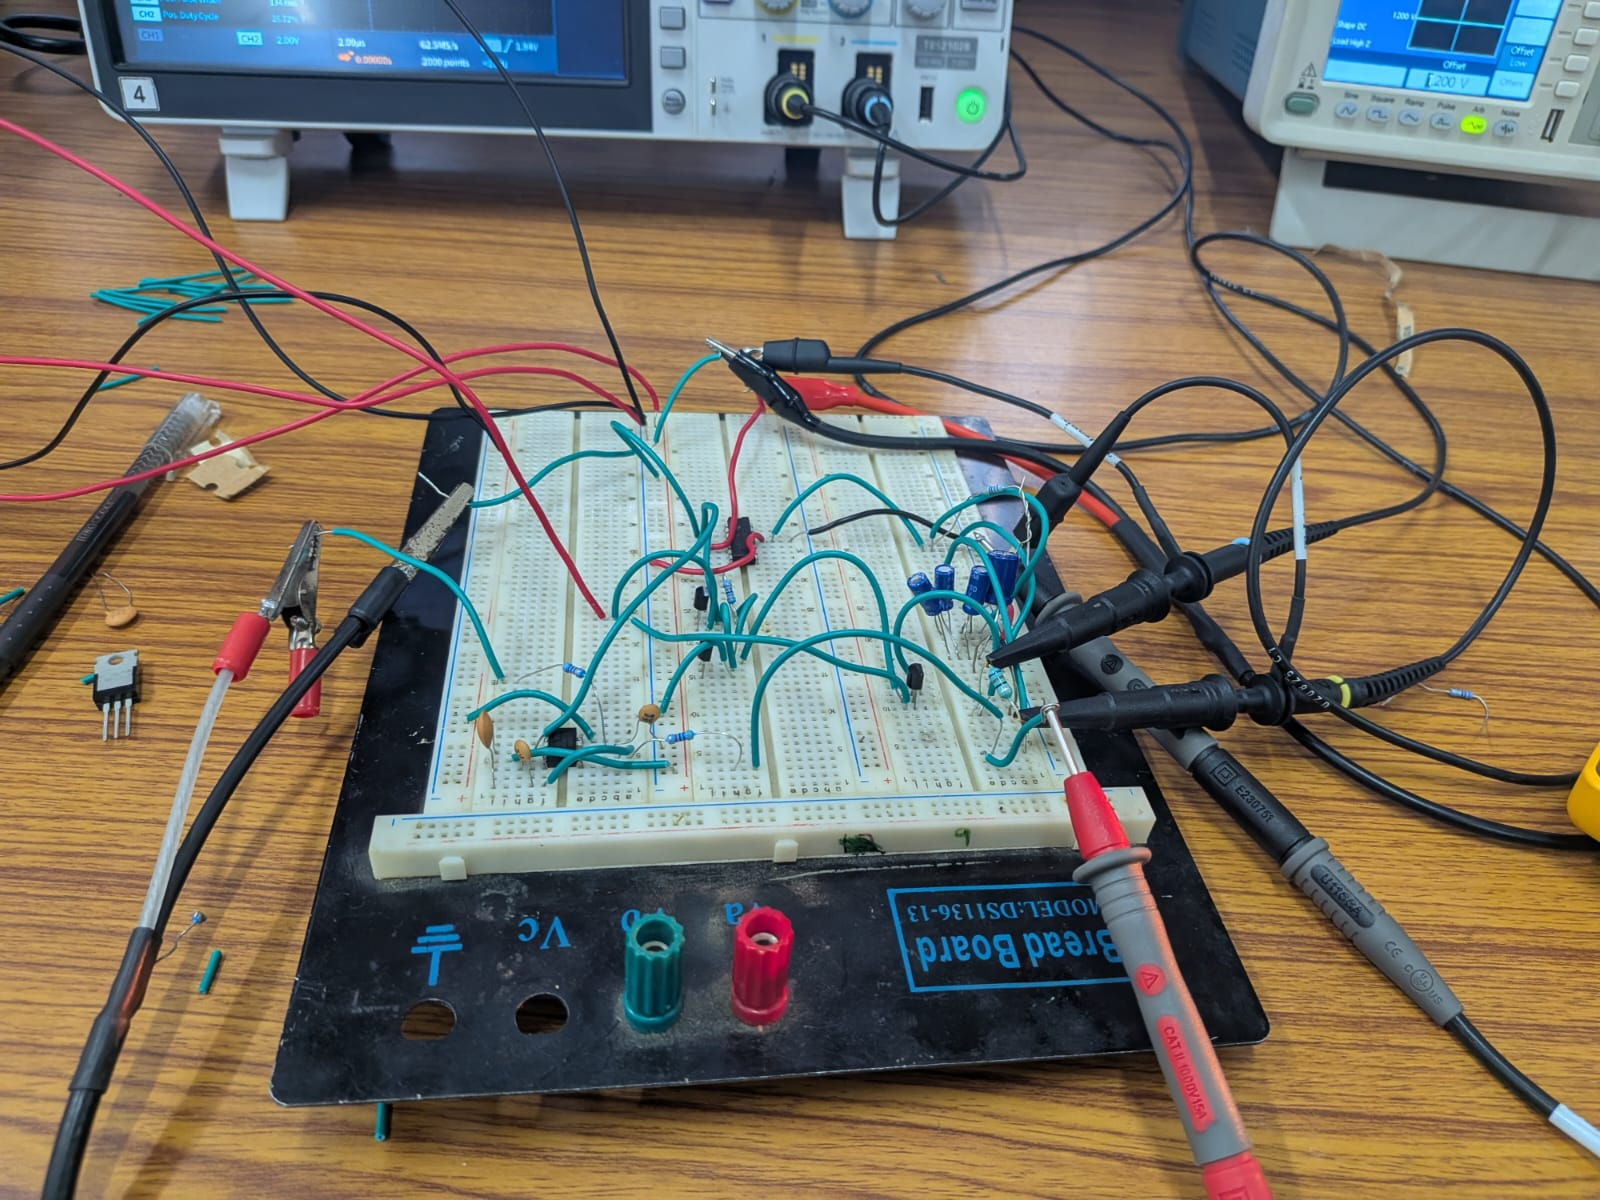
\includegraphics[width=\textwidth]{figures/bench_breadboard_top.jpg}
        \caption{Top-down view of the breadboard assembly.}
    \end{subfigure}
    \hfill
    \begin{subfigure}[b]{0.48\textwidth}
        \centering
        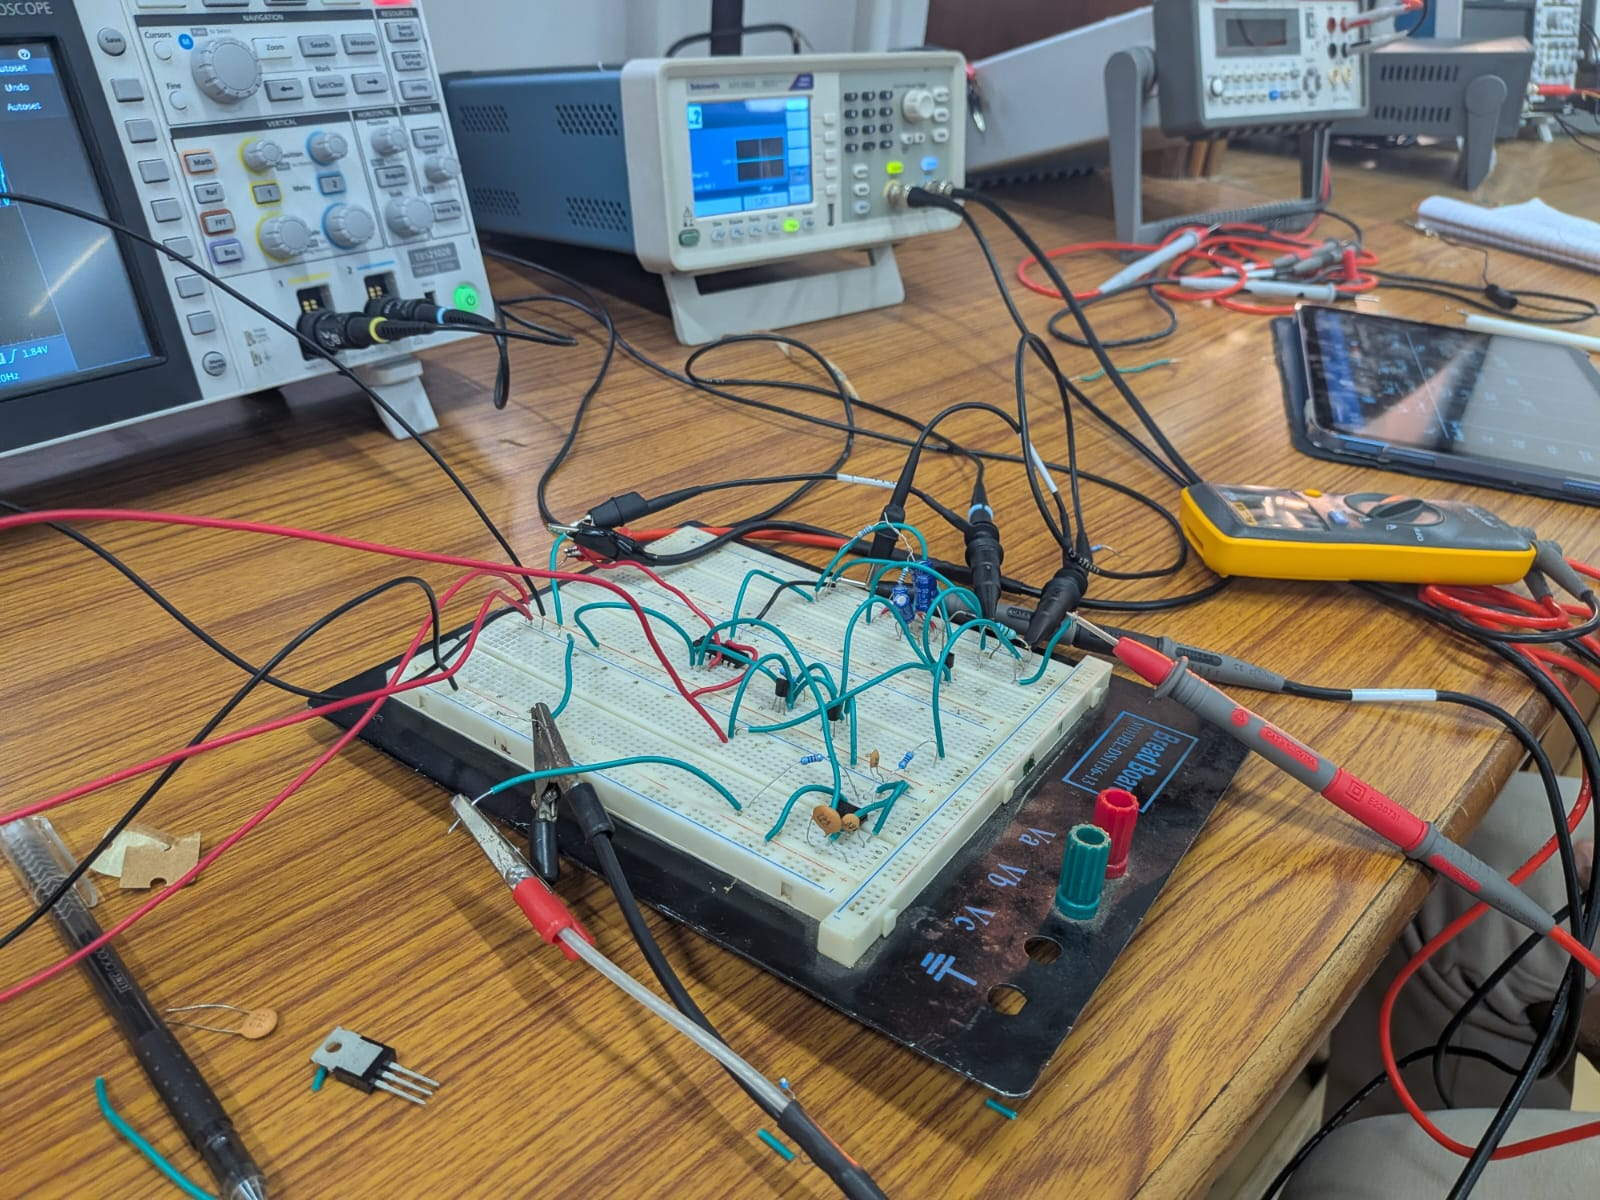
\includegraphics[width=\textwidth]{figures/bench_setup_wide.jpg}
        \caption{Full workbench instrumentation and probe routing.}
    \end{subfigure}
    \caption{Photographs of the physical hardware setup on the laboratory workbench showing the breadboard circuit, DSO, AFG, and digital multimeters.}
    \label{fig:bench_photos}
\end{figure}

% ==============================================================================
% Section 3: Theory & Operating Principle
% ==============================================================================
\section{Theoretical Background and Mathematical Modeling}
\label{sec:theory}

\subsection{Basic Buck Topology and Volt-Second Balance}
The step-down (buck) switching converter transfers electrical energy from a higher DC input potential $\Vin$ to a lower DC output potential $\Vout$ with high theoretical thermodynamic efficiency. Unlike a linear series-pass regulator where the excess input-to-output voltage drop $(\Vin - \Vout)$ is dropped across an active transistor operating in its linear active region (dissipating large thermal power $P_{\mathrm{diss}} = (\Vin - \Vout)\Iload$), a buck converter utilizes a transistor operating exclusively in switched saturation or cut-off.

The basic circuit comprises a high-side P-channel MOSFET switch $Q_1$, a freewheeling Schottky catch diode $D_1$, an energy storage inductor $L_1$, and a capacitive filter bank $C_{\mathrm{out}}$ shunting the load $\RL$, as illustrated in the complete schematic diagram of Figure~\ref{fig:full_schematic}.

\begin{figure}[H]
    \centering
    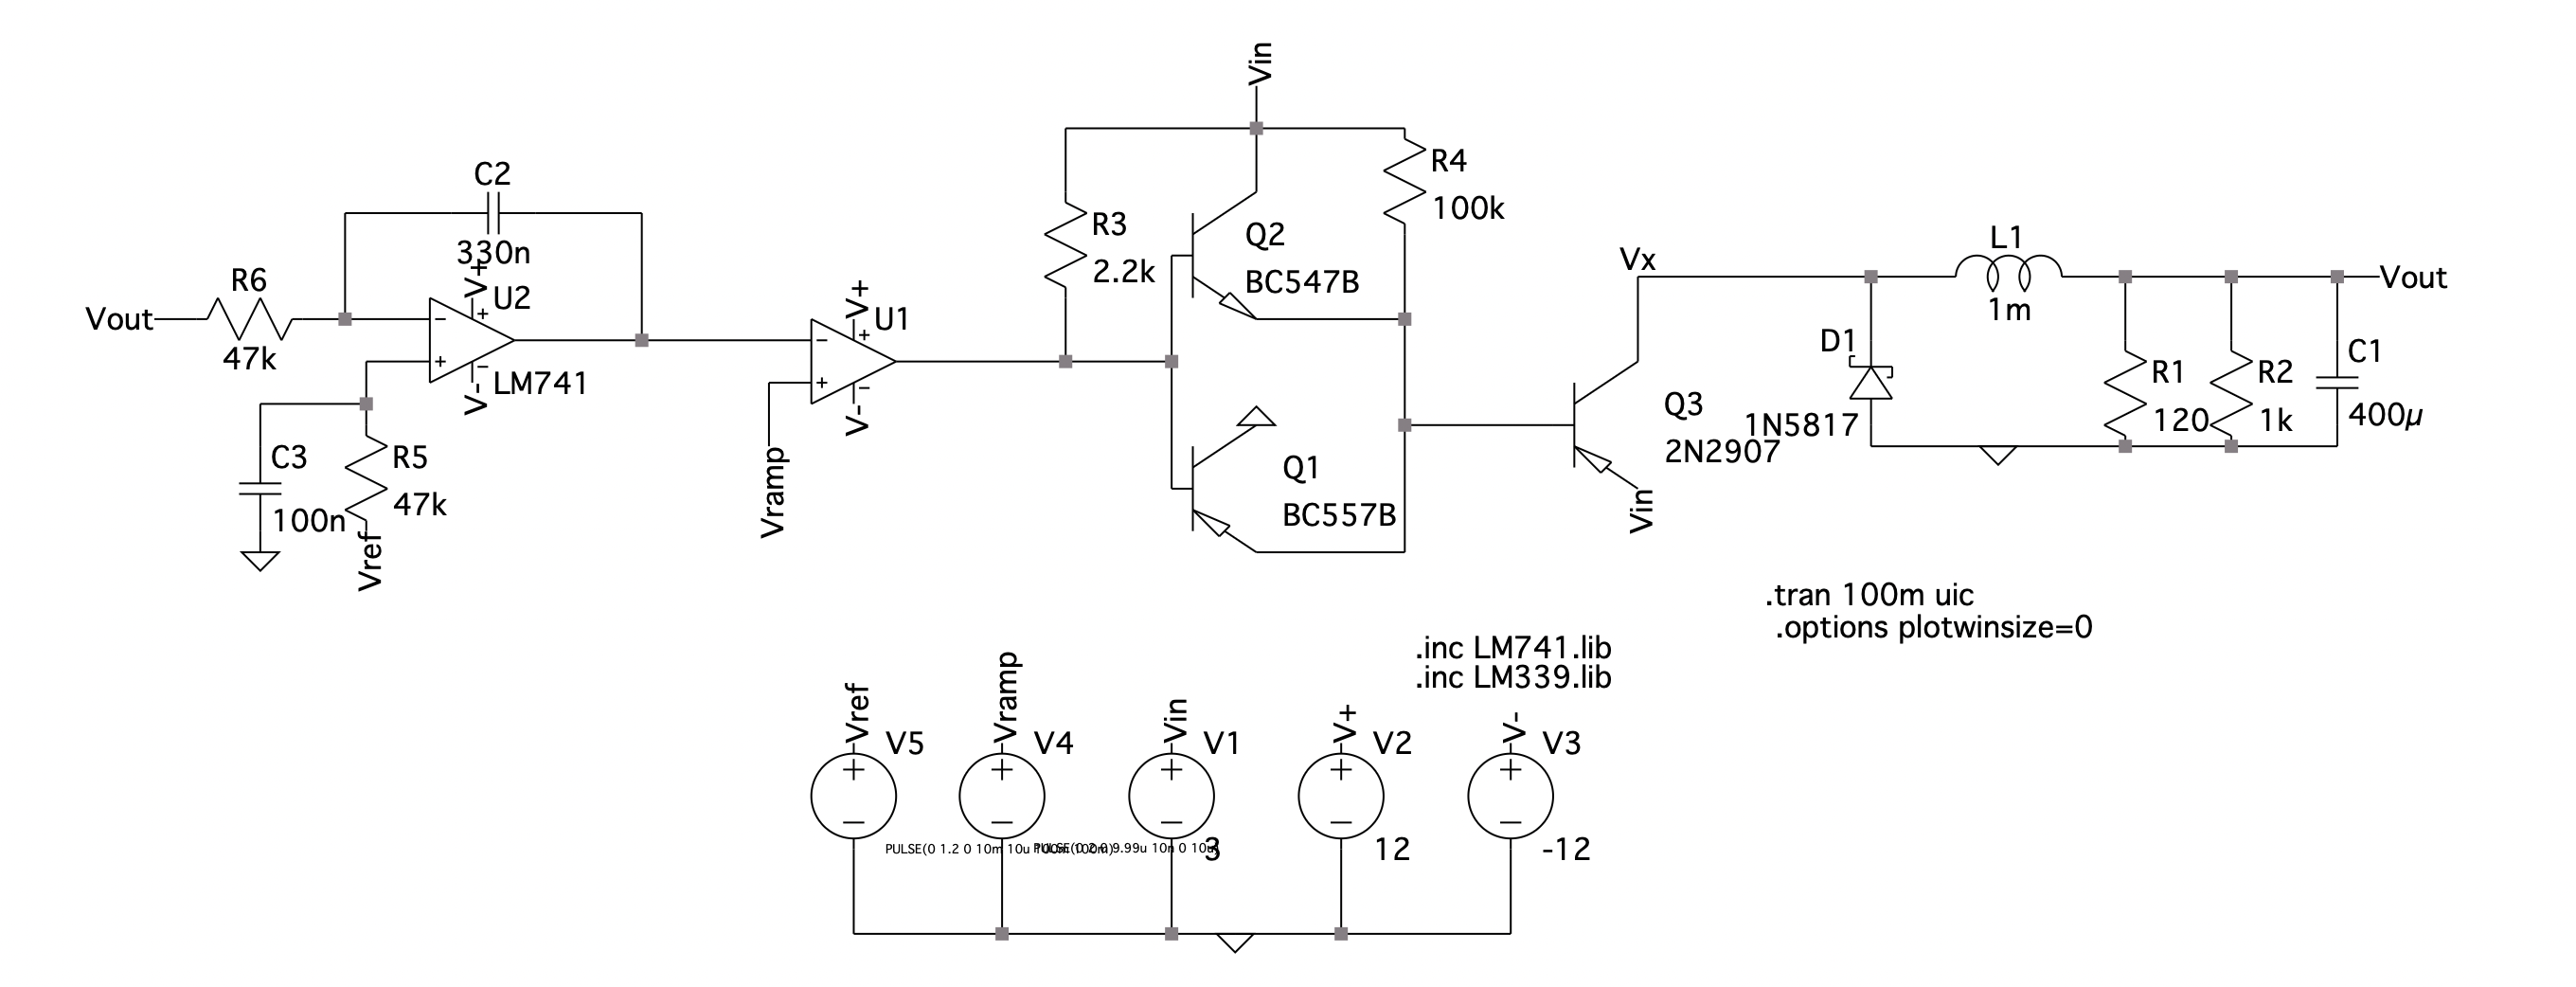
\includegraphics[width=0.88\linewidth]{figures/ltspice_part_c_ckt.png}
    \caption{Complete schematic diagram of the closed-loop PMOS buck regulator, detailing the LM741 integrator, LM339 comparator, BC547/BC557 complementary totem-pole gate driver, high-side power switch, and LC output filter.}
    \label{fig:full_schematic}
\end{figure}

Let the switching period be $T = 1/\fs$, where $\fs = 100\,\mathrm{kHz}$ is the switching frequency ($T = 10.0\,\mu\mathrm{s}$). The switch is turned ON for duration $t_{\mathrm{on}} = D \cdot T$ and turned OFF for duration $t_{\mathrm{off}} = (1 - D)T$, where $D \in [0, 1]$ represents the switching duty cycle.

\subsubsection{Switch ON State \texorpdfstring{($0 \le t < DT$)}{(0 <= t < DT)}}
When the gate of $Q_1$ is pulled to ground, $V_{GS} = -\Vin$, turning the P-MOSFET hard ON. The switch-node potential $\Vx$ rises to approximately $\Vin - I_L \Rdson$. The diode $D_1$ is reverse-biased by $\Vin$. The voltage across the inductor is:
\begin{equation}
    v_L(t) = \Vin - \Vout - I_L \Rdson \approx \Vin - \Vout
    \label{eq:vl_on}
\end{equation}
The inductor current ramps upward linearly according to Faraday's law:
\begin{equation}
    \frac{di_L}{dt} = \frac{\Vin - \Vout}{L_1} > 0
    \label{eq:dil_dt_on}
\end{equation}

\subsubsection{Switch OFF State \texorpdfstring{($DT \le t < T$)}{(DT <= t < T)}}
When $Q_1$ is turned OFF, the inductor current cannot discontinue instantaneously due to magnetic flux conservation. The inductor voltage flips polarity, forcing the switch-node voltage $\Vx$ below circuit ground until the Schottky catch diode $D_1$ becomes forward-biased at $-V_F$. The voltage across the inductor during this freewheeling phase is:
\begin{equation}
    v_L(t) = -(\Vout + V_F)
    \label{eq:vl_off}
\end{equation}
The inductor current ramps downward with slope:
\begin{equation}
    \frac{di_L}{dt} = -\frac{\Vout + V_F}{L_1} < 0
    \label{eq:dil_dt_off}
\end{equation}

\subsubsection{Volt-Second Balance Condition}
In periodic steady state, the net change in inductor magnetic flux over a complete switching cycle must be zero, otherwise the inductor core would experience net flux accumulation and saturate:
\begin{equation}
    \int_{0}^{T} v_L(t)\,dt = 0
    \label{eq:volt_sec}
\end{equation}
Substituting Equations~\eqref{eq:vl_on} and \eqref{eq:vl_off} into Equation~\eqref{eq:volt_sec}:
\begin{equation}
    (\Vin - \Vout) \cdot D T - (\Vout + V_F) \cdot (1 - D) T = 0
\end{equation}
Dividing by $T$ and collecting terms:
\begin{equation}
    D \Vin - D \Vout - \Vout - V_F + D \Vout + D V_F = 0
\end{equation}
\begin{equation}
    D(\Vin + V_F) = \Vout + V_F
\end{equation}
Thus, the exact relationship between duty cycle $D$, input voltage $\Vin$, diode forward drop $V_F$, and output voltage $\Vout$ under Continuous Conduction Mode (CCM) is:
\begin{equation}
    D = \frac{\Vout + V_F}{\Vin + V_F}
    \label{eq:duty_exact}
\end{equation}
For an ideal diode ($V_F \to 0$), Equation~\eqref{eq:duty_exact} simplifies to the familiar ideal buck relation:
\begin{equation}
    D_{\mathrm{ideal}} = \frac{\Vout}{\Vin} \iff \Vout = D \cdot \Vin
    \label{eq:duty_ideal}
\end{equation}
Conversely, when an open-loop switching stage is driven with a known duty cycle $D$, the predicted output voltage taking diode drop into account is:
\begin{equation}
    \Vout = D(\Vin + V_F) - V_F
    \label{eq:vout_from_d}
\end{equation}

\subsection{Inductor Ripple Current and Conduction Modes}
The peak-to-peak inductor ripple current $\dI$ represents the total AC current swing through the magnetic element. Since the current falls during the OFF duration $t_{\mathrm{off}} = (1 - D)T$ at rate $(\Vout + V_F)/L_1$:
\begin{equation}
    \dI = \left(\frac{\Vout + V_F}{L_1}\right) (1 - D) T = \frac{(\Vout + V_F)(1 - D)}{L_1 \fs}
    \label{eq:ripple_current}
\end{equation}
Because $(1 - D)$ is largest when $D$ is smallest (which occurs at the maximum line voltage $\Vin = 5.0\,\mathrm{V}$), the maximum inductor ripple current occurs at $\Vin = 5.0\,\mathrm{V}$.

\subsubsection{Continuous vs. Discontinuous Conduction Mode (CCM vs. DCM)}
The inductor current waveform consists of a DC average component equal to the load current $\Iload$ plus the triangular AC ripple:
\begin{equation}
    i_L(t) = \Iload + \tilde{i}_L(t), \quad \text{where} \quad \max(i_L) = \Iload + \frac{\dI}{2}, \quad \min(i_L) = \Iload - \frac{\dI}{2}
\end{equation}
\begin{itemize}[leftmargin=1.5em]
    \item \textbf{Continuous Conduction Mode (CCM):} When the load current exceeds half of the ripple current ($\Iload > \dI / 2$), the minimum current remains positive ($\min(i_L) > 0$). The inductor conducts uninterrupted current throughout the entire switching cycle.
    \item \textbf{Critical Conduction Boundary ($I_{\mathrm{crit}}$):} The boundary between CCM and DCM occurs precisely when the valley of the inductor current touches zero:
    \begin{equation}
        I_{\mathrm{crit}} = \frac{\dI}{2} = \frac{(\Vout + V_F)(1 - D)}{2 L_1 \fs}
        \label{eq:icrit}
    \end{equation}
    \item \textbf{Discontinuous Conduction Mode (DCM):} When the load current falls below $I_{\mathrm{crit}}$ ($\Iload < \dI / 2$), the inductor current drops to zero before the end of the switching period ($t_{\mathrm{off}}$). Because the Schottky diode cannot conduct negative current, it turns off. During this remaining idle interval $t_{\mathrm{idle}}$, the inductor current remains clamped at zero, and the switch-node $\Vx$ floats, forming an undamped resonant tank with the parasitic capacitances of the MOSFET and diode, producing high-frequency sinusoidal ringing at frequency:
    \begin{equation}
        f_{\mathrm{ring}} = \frac{1}{2\pi \sqrt{L_1 C_x}}
        \label{eq:fring}
    \end{equation}
    where $C_x \approx C_{\mathrm{oss,Q}} + C_{j,\mathrm{diode}} + C_{\mathrm{stray}}$.
\end{itemize}

\subsection{Output Voltage Ripple Mechanics and Filtering}
The AC component of the inductor current $\tilde{i}_L(t)$ must be absorbed entirely by the output capacitor bank, as the resistive load draws steady DC current. The resulting peak-to-peak output voltage ripple $\Delta \Vout$ is composed of two orthogonal physical components:
\begin{equation}
    \Delta \Vout = \Delta V_{C,\mathrm{capacitive}} + \Delta V_{\mathrm{ESR}}
    \label{eq:ripple_components}
\end{equation}

\subsubsection{Capacitive Charging Ripple \texorpdfstring{($\Delta V_{C}$)}{(Delta VC)}}
During the interval when $i_L(t) > \Iload$, excess charge accumulates on the output capacitor plates. The geometry of the triangular current waveform implies that the total charge accumulated is the area of the upper triangular lobe:
\begin{equation}
    \Delta Q = \frac{1}{2} \left(\frac{T}{2}\right) \left(\frac{\dI}{2}\right) = \frac{\dI \cdot T}{8} = \frac{\dI}{8 \fs}
\end{equation}
The peak-to-peak capacitive voltage variation is therefore:
\begin{equation}
    \Delta V_{C} = \frac{\Delta Q}{C_{\mathrm{out}}} = \frac{\dI}{8 \fs C_{\mathrm{out}}}
    \label{eq:dvc}
\end{equation}

\subsubsection{Resistive ESR Ripple \texorpdfstring{($\Delta V_{\mathrm{ESR}}$)}{(Delta VESR)}}
The capacitor possesses an inherent equivalent series resistance ($\ESR$). As the full inductor ripple current $\dI$ flows through this parasitic resistance, an instantaneous ohmic IR drop is generated across the terminals:
\begin{equation}
    \Delta V_{\mathrm{ESR}} = \dI \cdot \ESR
    \label{eq:dvesr}
\end{equation}
Because the peak of the ESR voltage coincides with the peak of the current while the capacitive ripple is in phase quadrature (displaced by $90^\circ$), the linear upper bound on total ripple voltage is:
\begin{equation}
    \Delta \Vout \le \dI \left( \ESR + \frac{1}{8 \fs C_{\mathrm{out}}} \right)
    \label{eq:total_ripple}
\end{equation}

\subsubsection{The 0.1\% Ripple Limit and Parallel Capacitor Bank Design}
The lab specification requires $\Delta \Vout \le 0.1\% \times 1.2\,\mathrm{V} = 1.20\,\mathrm{mV}_{\mathrm{p\text{-}p}}$.
For a $400\,\mu\mathrm{F}$ capacitance at $\fs = 100\,\mathrm{kHz}$:
\begin{equation}
    \frac{1}{8 \fs C_{\mathrm{out}}} = \frac{1}{8 \times 10^5 \times 400 \times 10^{-6}} = \frac{1}{320} \approx 3.125\,\mathrm{m}\Omega
\end{equation}
With $\dI \approx 16.3\,\mathrm{mA}$, the capacitive ripple contribution is negligible:
\begin{equation}
    \Delta V_C = 16.3\,\mathrm{mA} \times 3.125\,\mathrm{m}\Omega \approx 0.051\,\mathrm{mV}
\end{equation}
Hence, \textbf{the output ripple is completely dominated by the capacitor ESR}:
\begin{equation}
    \Delta \Vout \approx \dI \cdot \ESR
\end{equation}
To achieve $\Delta \Vout \le 1.2\,\mathrm{mV}$, the maximum allowable ESR is:
\begin{equation}
    \ESR_{\mathrm{max}} \le \frac{1.2\,\mathrm{mV} - 0.051\,\mathrm{mV}}{16.3\,\mathrm{mA}} \approx 70.5\,\mathrm{m}\Omega
\end{equation}
Because a standard single $100\,\mu\mathrm{F}$ electrolytic capacitor typically exhibits an ESR between $200\,\mathrm{m}\Omega$ and $500\,\mathrm{m}\Omega$ (which would produce $3.3\text{--}8.2\,\mathrm{mV}$ ripple, failing the specification), connecting $N = 4$ identical capacitors in parallel divides the effective ESR by four:
\begin{equation}
    \ESR_{\mathrm{eff}} = \frac{\ESR_{\mathrm{single}}}{N} = \frac{100\,\mathrm{m}\Omega}{4} = 25.0\,\mathrm{m}\Omega
\end{equation}
This yields a theoretical switching ripple of $16.3\,\mathrm{mA} \times 25\,\mathrm{m}\Omega \approx 0.41\,\mathrm{mV}_{\mathrm{p\text{-}p}}$, providing a healthy theoretical factor-of-three safety margin.

\subsection{Pulse-Width Modulator Operation}
The duty cycle $D$ is synthesized using a voltage comparator (LM339). The inverting input of the comparator receives a slowly varying DC control voltage $\Vc$ from the error amplifier. The non-inverting input receives a periodic ramp waveform $\Vramp(t)$ running from $0\,\mathrm{V}$ to $V_{p} = 2.0\,\mathrm{V}$ at frequency $\fs = 100\,\mathrm{kHz}$.

\begin{figure}[H]
    \centering
    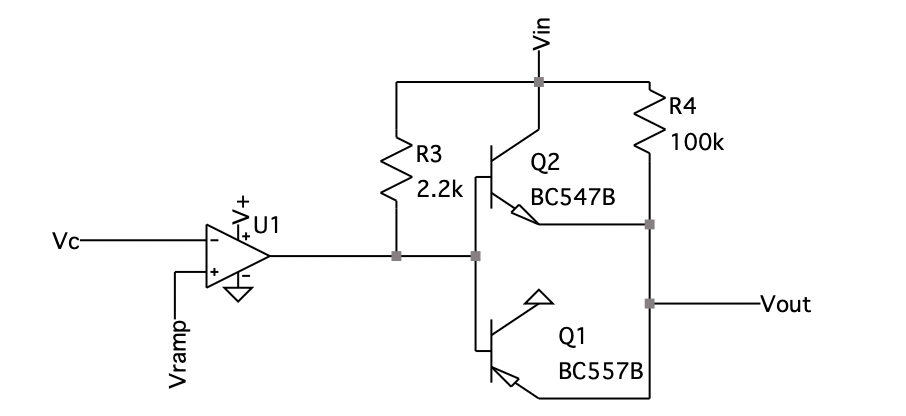
\includegraphics[width=0.75\linewidth]{figures/ltspice_part_a_ckt.png}
    \caption{LTspice schematic of Part A: The PWM modulator circuit utilizing the LM339 comparator with $2.2\,\mathrm{k}\Omega$ pull-up and BC547/BC557 complementary emitter-follower gate buffer.}
    \label{fig:part_a_schematic}
\end{figure}

The comparator output is pulled low whenever the ramp voltage is below the control voltage ($\Vramp(t) < \Vc$). Because the P-channel power MOSFET conducts when its gate is pulled low, the switch ON time corresponds directly to the comparator LOW duration:
\begin{equation}
    t_{\mathrm{on}} = T \cdot \left(\frac{\Vc}{V_p}\right) \implies D = \frac{\Vc}{V_p} = \frac{\Vc}{2.0\,\mathrm{V}}
    \label{eq:d_modulator}
\end{equation}
If $\Vout$ droops below $\Vref$, the error amplifier ramps $\Vc$ upward, increasing $D$ and driving more energy into the LC filter to restore $\Vout$.

\subsection{Control Loop Architecture and Integral Compensation}
The small-signal transfer function of the uncompensated LC output filter is a second-order low-pass filter:
\begin{equation}
    G_{\mathrm{filter}}(s) = \frac{\Vout(s)}{\Vx(s)} \approx \frac{1}{1 + s \frac{L_1}{\RL} + s^2 L_1 C_{\mathrm{out}}}
\end{equation}
The complex conjugate poles resonate at the undamped corner frequency:
\begin{equation}
    f_o = \frac{1}{2\pi \sqrt{L_1 C_{\mathrm{out}}}} = \frac{1}{2\pi \sqrt{1.0\times 10^{-3} \times 400\times 10^{-6}}} \approx 251.6\,\mathrm{Hz}
    \label{eq:fo_res}
\end{equation}
At resonance, the phase angle plummets abruptly by $180^\circ$. If the feedback loop crossover frequency were placed near or above $305\,\mathrm{Hz}$, the $-180^\circ$ phase lag from the LC filter, combined with the $-90^\circ$ phase lag of the error amplifier and comparator delays, would exceed $-360^\circ$ (Barkhausen criterion), causing catastrophic closed-loop oscillation.

To ensure unconditional stability without requiring complex multi-zero lead compensation (Type-III), an \textbf{integrator compensator} is constructed around the LM741 operational amplifier with feedback capacitor $C_i = 330\,\mathrm{nF}$ and input resistor $R_1 = 47\,\mathrm{k}\Omega$. The transfer function of the integrator is:
\begin{equation}
    A_I(s) = -\frac{1}{s R_1 C_i}
\end{equation}
The loop transmission is given by:
\begin{equation}
    T(s) = \left(\frac{\Vin}{V_p}\right) \cdot \left(\frac{1}{s R_1 C_i}\right) \cdot G_{\mathrm{filter}}(s)
\end{equation}
Setting the loop gain magnitude $|T(j 2\pi f_c)| = 1$ well below $f_o$ (where $G_{\mathrm{filter}} \approx 1$):
\begin{equation}
    f_c = \frac{\Vin}{V_p} \frac{1}{2\pi R_1 C_i}
    \label{eq:fc}
\end{equation}
For $\Vin = 3.0\,\mathrm{V}$ to $5.0\,\mathrm{V}$:
\begin{equation}
    f_c(3\,\mathrm{V}) = \frac{3.0}{2.0} \frac{1}{2\pi \times 47\times 10^3 \times 330\times 10^{-9}} = 1.5 \times 10.26\,\mathrm{Hz} \approx 15.4\,\mathrm{Hz}
\end{equation}
\begin{equation}
    f_c(5\,\mathrm{V}) = \frac{5.0}{2.0} \frac{1}{2\pi \times 47\times 10^3 \times 330\times 10^{-9}} = 2.5 \times 10.26\,\mathrm{Hz} \approx 25.7\,\mathrm{Hz}
\end{equation}
Because $f_c \ll f_o$ ($15\text{--}26\,\mathrm{Hz} \ll 252\,\mathrm{Hz}$), the loop crosses unity gain where the phase margin is nearly $90^\circ$, rendering the converter unconditionally stable against load and line variations. The trade-off is a deliberately sluggish transient response (settling time $\sim 20\text{--}35\,\mathrm{ms}$).

\subsubsection{Op-Amp Input Bias Balancing}
The LM741 utilizes bipolar junction input transistors with an input bias current $I_B \approx 80\text{--}500\,\mathrm{nA}$. Flowing through the $47\,\mathrm{k}\Omega$ input resistor, $I_B$ would produce an uncompensated DC offset error of $I_B \cdot R_1 \approx 4\text{--}24\,\mathrm{mV}$. To neutralize this error, an identical resistor $R_3 = 47\,\mathrm{k}\Omega$ is placed in series with the non-inverting terminal (pin 3), bypassed by $C_3 = 100\,\mathrm{nF}$ to ground. The common-mode bias currents create matching voltage drops across both inputs, leaving only the tiny input offset voltage ($V_{os} \approx 1\,\mathrm{mV}$) and offset current error ($I_{os} R_1 \approx 1\,\mathrm{mV}$).

\subsection{High-Side P-MOSFET Gate Drive and Buffer Action}
A crucial advantage of employing a P-channel MOSFET for the high-side switch rather than an N-channel device is the simplification of the gate driver:
\begin{itemize}[leftmargin=1.5em]
    \item \textbf{Drive Mechanics:} The source of $Q_1$ is connected directly to $\Vin$. To turn $Q_1$ OFF, the gate is pulled to $\Vin$, giving $V_{GS} = 0\,\mathrm{V}$. To turn $Q_1$ ON, the gate is pulled to ground ($0\,\mathrm{V}$), giving $V_{GS} = -\Vin$ ($-3.0\,\mathrm{V}$ to $-5.0\,\mathrm{V}$). Thus, the gate voltage never needs to exceed $\Vin$, completely eliminating the need for a bootstrap capacitor, high-side charge pump, or isolated floating gate driver supply.
    \item \textbf{Gate Driver Buffer:} The LM339 comparator has an open-collector output with limited sinking current ($\sim 16\,\mathrm{mA}$) and relies on a $2.2\,\mathrm{k}\Omega$ pull-up resistor to charge the gate capacitance. If connected directly to the gate, the pull-up RC charging time constant would be $\tau = 2.2\,\mathrm{k}\Omega \times 1.5\,\mathrm{nF} \approx 3.3\,\mu\mathrm{s}$, which is a huge fraction of the $10\,\mu\mathrm{s}$ period and would cause catastrophic switching dissipation.
    \item \textbf{Totem-Pole Emitter Followers:} The complementary pair BC547B (NPN) and BC557B (PNP) acts as a low-impedance current-boosting buffer. When the comparator turns OFF, the NPN pulls the gate rapidly to $\Vin - V_{BE}$; when the comparator pulls down, the PNP pulls the gate rapidly to $0\,\mathrm{V} + V_{BE}$. This slashes the switching transition times ($t_r, t_f$) to approximately $60\text{--}70\,\mathrm{ns}$.
\end{itemize}

\subsection{Power Loss Budget and Efficiency Modeling}
Power dissipation in the buck switching regulator is distributed among five distinct physical mechanisms:
\begin{enumerate}[leftmargin=1.5em]
    \item \textbf{P-MOSFET Conduction Loss ($P_{\mathrm{cond},Q}$):} Occurs during the switch ON time:
    \begin{equation}
        P_{\mathrm{cond},Q} = D \cdot I_{\mathrm{RMS}}^2 \cdot \Rdson \approx D \cdot \Iload^2 \cdot \Rdson
    \end{equation}
    \item \textbf{Schottky Diode Conduction Loss ($P_{\mathrm{cond},D}$):} Occurs during the freewheeling phase:
    \begin{equation}
        P_{\mathrm{cond},D} = (1 - D) \cdot \Iload \cdot V_F
    \end{equation}
    \item \textbf{Inductor Series Winding Loss ($P_{L}$):} Ohmic heating in the copper wire of the choke:
    \begin{equation}
        P_{L} = I_{\mathrm{RMS}}^2 \cdot \DCR \approx \Iload^2 \cdot \DCR
    \end{equation}
    \item \textbf{Switching Overlap Loss ($P_{\mathrm{sw}}$):} During turn-on and turn-off, $V_{DS}$ and $I_D$ overlap simultaneously:
    \begin{equation}
        P_{\mathrm{sw}} = \frac{1}{2} \Vin \Iload (t_r + t_f) \fs
    \end{equation}
    \item \textbf{Gate Drive Loss ($P_{\mathrm{gate}}$):} Energy required to charge and discharge the gate capacitance $Q_g$ each cycle, drawn from $\Vin$:
    \begin{equation}
        P_{\mathrm{gate}} = Q_g \cdot \Vin \cdot \fs
    \end{equation}
\end{enumerate}
Total power stage losses are:
\begin{equation}
    P_{\mathrm{loss,stage}} = P_{\mathrm{cond},Q} + P_{\mathrm{cond},D} + P_{L} + P_{\mathrm{sw}} + P_{\mathrm{gate}}
\end{equation}
The \textbf{power stage efficiency} is:
\begin{equation}
    \eta_{\mathrm{stage}} = \frac{\Pout}{\Pin} = \frac{\Vout \Iload}{\Vin \Iin}
\end{equation}
The \textbf{total system efficiency}, which incorporates the quiescent operating power of the operational amplifier and comparator control circuitry drawn from the auxiliary $\pm12\,\mathrm{V}$ supplies ($P_{\mathrm{AUX}} = 12\,\mathrm{V} \cdot I_{+12\mathrm{V}} + 12\,\mathrm{V} \cdot I_{-12\mathrm{V}}$), is:
\begin{equation}
    \eta_{\mathrm{total}} = \frac{\Pout}{\Pin + P_{\mathrm{AUX}}} = \frac{\Vout \Iload}{\Vin \Iin + P_{\mathrm{AUX}}}
\end{equation}

% ==============================================================================
% Section 4: Design Calculations
% ==============================================================================
\section{Design Calculations}
\label{sec:calculations}

Using the measured and bench-verified component parameters ($\fs = 100\,\mathrm{kHz}$, $L_1 = 1.0\,\mathrm{mH}$, $\DCR = 0.80\,\Omega$, $C_{\mathrm{out}} = 400\,\mu\mathrm{F}$, $\ESR = 25.0\,\mathrm{m}\Omega$, $V_F = 0.32\,\mathrm{V}$, $V_p = 2.00\,\mathrm{V}$, $R_1 = R_3 = 47\,\mathrm{k}\Omega$, $C_i = 330\,\mathrm{nF}$, and full load $\Iload = 100\,\mathrm{mA}$ with $\Vout = 1.200\,\mathrm{V}$), the exact theoretical design quantities are evaluated below.

\subsection{Operating Duty Cycle}
Applying Equation~\eqref{eq:duty_exact}:
\begin{itemize}
    \item At $\Vin = 3.0\,\mathrm{V}$:
    \begin{equation*}
        D(3.0\,\mathrm{V}) = \frac{1.200 + 0.32}{3.000 + 0.32} = \frac{1.520}{3.320} \approx \mathbf{0.4578} \quad (45.78\%)
    \end{equation*}
    \item At $\Vin = 5.0\,\mathrm{V}$:
    \begin{equation*}
        D(5.0\,\mathrm{V}) = \frac{1.200 + 0.32}{5.000 + 0.32} = \frac{1.520}{5.320} \approx \mathbf{0.2857} \quad (28.57\%)
    \end{equation*}
\end{itemize}

\subsection{Inductor Current Ripple and Critical Current}
Applying Equation~\eqref{eq:ripple_current}:
\begin{itemize}
    \item At $\Vin = 3.0\,\mathrm{V}$:
    \begin{align*}
        \dI(3.0\,\mathrm{V}) &= \frac{(1.20 + 0.32)(1 - 0.4578)}{1.0\times 10^{-3} \times 10^5} = \frac{0.8241}{100.0} \approx \mathbf{8.24\,\mathrm{mA}} \\
        I_{\mathrm{crit}}(3.0\,\mathrm{V}) &= \frac{\dI}{2} \approx \mathbf{4.12\,\mathrm{mA}}
    \end{align*}
    \item At $\Vin = 5.0\,\mathrm{V}$:
    \begin{align*}
        \dI(5.0\,\mathrm{V}) &= \frac{(1.20 + 0.32)(1 - 0.2857)}{1.0\times 10^{-3} \times 10^5} = \frac{1.0857}{100.0} \approx \mathbf{10.86\,\mathrm{mA}} \\
        I_{\mathrm{crit}}(5.0\,\mathrm{V}) &= \frac{\dI}{2} \approx \mathbf{5.43\,\mathrm{mA}}
    \end{align*}
    \begin{equation*}
        I_{\mathrm{crit}}(5.0\,\mathrm{V}) = \frac{\dI}{2} \approx \mathbf{8.15\,\mathrm{mA}}
    \end{equation*}
\end{itemize}
Because full load current $\Iload = 100\,\mathrm{mA} \gg I_{\mathrm{crit}}$, the converter operates securely in Continuous Conduction Mode (CCM) across all line voltages at full load.

\subsection{Output Voltage Ripple}
Using Equation~\eqref{eq:total_ripple} with $C_{\mathrm{out}} = 400\,\mu\mathrm{F}$ and $\ESR = 25.0\,\mathrm{m}\Omega$:
\begin{equation*}
    \text{Capacitive term: } \frac{1}{8 \fs C_{\mathrm{out}}} = \frac{1}{8 \times 10^5 \times 400\times 10^{-6}} = 3.125\,\mathrm{m}\Omega
\end{equation*}
\begin{itemize}
    \item At $\Vin = 3.0\,\mathrm{V}$ ($\dI = 12.12\,\mathrm{mA}$):
    \begin{equation*}
        \Delta \Vout = 12.12\,\mathrm{mA} \times (25.0\,\mathrm{m}\Omega + 3.125\,\mathrm{m}\Omega) = 12.12\,\mathrm{mA} \times 28.125\,\mathrm{m}\Omega \approx \mathbf{0.341\,\mathrm{mV}_{\mathrm{p\text{-}p}}}
    \end{equation*}
    \item At $\Vin = 5.0\,\mathrm{V}$ ($\dI = 15.97\,\mathrm{mA}$):
    \begin{equation*}
        \Delta \Vout = 15.97\,\mathrm{mA} \times 28.125\,\mathrm{m}\Omega \approx \mathbf{0.449\,\mathrm{mV}_{\mathrm{p\text{-}p}}}
    \end{equation*}
\end{itemize}
Both theoretical values are comfortably below the $1.20\,\mathrm{mV}_{\mathrm{p\text{-}p}}$ specification limit ($0.1\%$).

\subsection{Maximum Allowable Capacitor ESR}
To strictly satisfy the $1.20\,\mathrm{mV}_{\mathrm{p\text{-}p}}$ ripple limit at the worst-case line voltage ($\Vin = 5.0\,\mathrm{V}$):
\begin{equation}
    \ESR_{\mathrm{max}} \le \frac{\Delta V_{\mathrm{limit}}}{\dI} - \frac{1}{8 \fs C_{\mathrm{out}}} = \frac{1.20\,\mathrm{mV}}{16.0\,\mathrm{mA}} - 3.125\,\mathrm{m}\Omega = 75.0\,\mathrm{m}\Omega - 3.125\,\mathrm{m}\Omega = \mathbf{71.87\,\mathrm{m}\Omega}
\end{equation}

\subsection{Loop Resonance and Integrator Crossover Frequency}
The output filter double pole is located at:
\begin{equation*}
    f_o = \frac{1}{2\pi \sqrt{L_1 C_{\mathrm{out}}}} = \frac{1}{2\pi \sqrt{1.0\times 10^{-3} \times 400\times 10^{-6}}} = \mathbf{251.6\,\mathrm{Hz}}
\end{equation*}
The integrator time constant is $\tau = R_1 C_i = 47\,\mathrm{k}\Omega \times 330\,\mathrm{nF} = 15.51\,\mathrm{ms}$.
The unity-gain frequency of the error integrator is:
\begin{equation*}
    f_u = \frac{1}{2\pi R_1 C_i} = \frac{1}{2\pi \times 15.51\times 10^{-3}} = \mathbf{10.26\,\mathrm{Hz}}
\end{equation*}
The loop crossover frequency spans:
\begin{equation*}
    f_c(3\,\mathrm{V}) = \frac{3.0}{2.0} \times 10.26\,\mathrm{Hz} = \mathbf{15.39\,\mathrm{Hz}}, \quad f_c(5\,\mathrm{V}) = \frac{5.0}{2.0} \times 10.26\,\mathrm{Hz} = \mathbf{25.65\,\mathrm{Hz}}
\end{equation*}
Because $f_c \approx 0.05\text{--}0.08\,f_o$, the loop transmission rolls off to unity gain long before the $-180^\circ$ phase drop of the LC resonant tank, ensuring absolute stability.

\subsection{Loss Budget Breakdown at \texorpdfstring{$\Vin = 5.0\,\mathrm{V}$, $\Iload = 100\,\mathrm{mA}$}{(Vin = 5.0V, Iload = 100mA)}}
With $D = 0.2857$, $(1 - D) = 0.7143$, $\Rdson = 1.60\,\Omega$, $V_F = 0.47\,\mathrm{V}$ at $100\,\mathrm{mA}$, $\DCR = 0.80\,\Omega$, $t_r + t_f = 130\,\mathrm{ns}$, and $Q_g = 2.0\,\mathrm{nC}$:
\begin{enumerate}
    \item \textbf{Diode Conduction Loss:} $P_{\mathrm{cond},D} = (1 - D)\Iload V_F = 0.7143 \times 0.10 \times 0.47 = \mathbf{33.57\,\mathrm{mW}}$
    \item \textbf{Inductor DCR Loss:} $P_L = \Iload^2 \DCR = (0.10)^2 \times 0.80 = \mathbf{8.00\,\mathrm{mW}}$
    \item \textbf{MOSFET Conduction Loss:} $P_{\mathrm{cond},Q} = D \Iload^2 \Rdson = 0.2857 \times (0.10)^2 \times 1.60 = \mathbf{4.57\,\mathrm{mW}}$
    \item \textbf{MOSFET Switching Loss:} $P_{\mathrm{sw}} = \frac{1}{2} \Vin \Iload (t_r + t_f) \fs = 0.5 \times 5.0 \times 0.10 \times 130\times 10^{-9} \times 10^5 = \mathbf{3.25\,\mathrm{mW}}$
    \item \textbf{Gate Drive Loss:} $P_{\mathrm{gate}} = Q_g \Vin \fs = 2.0\times 10^{-9} \times 5.0 \times 10^5 = \mathbf{1.00\,\mathrm{mW}}$
\end{enumerate}
Total power stage losses are $P_{\mathrm{loss,stage}} = 33.57 + 8.00 + 4.57 + 3.25 + 1.00 = \mathbf{50.39\,\mathrm{mW}}$.
Delivered output power is $\Pout = 1.200\,\mathrm{V} \times 0.10\,\mathrm{A} = \mathbf{120.0\,\mathrm{mW}}$.
Total input power is $\Pin = \Pout + P_{\mathrm{loss,stage}} = 120.0 + 50.39 = \mathbf{170.39\,\mathrm{mW}}$.
Predicted power stage efficiency is:
\begin{equation}
    \eta_{\mathrm{stage,pred}} = \frac{120.0\,\mathrm{mW}}{170.39\,\mathrm{mW}} \times 100\% = \mathbf{70.43\%}
\end{equation}

Table~\ref{tab:design_summary} collates these design formulas, theoretical targets, and bench implementation values.

\begin{table}[H]
\centering
\small
\caption{Summary of analytical design formulas and calculated design parameters.}
\label{tab:design_summary}
\renewcommand{\arraystretch}{1.25}
\begin{tabularx}{\linewidth}{lXrr}
\toprule
\textbf{Quantity} & \textbf{Analytical Expression} & \textbf{Value at 3.0\,V} & \textbf{Value at 5.0\,V} \\
\midrule
Duty cycle $D$ & $(\Vout + V_F)/(\Vin + V_F)$ & 0.4578 (45.8\%) & 0.2857 (28.6\%) \\
Inductor ripple current $\dI$ & $(\Vout + V_F)(1 - D)/(L_1 \fs)$ & $12.12\,\mathrm{mA}$ & $15.97\,\mathrm{mA}$ \\
Critical current $I_{\mathrm{crit}}$ & $\dI / 2$ & $6.06\,\mathrm{mA}$ & $8.15\,\mathrm{mA}$ \\
Capacitive ripple $\Delta V_C$ & $\dI / (8 \fs C_{\mathrm{out}})$ & $0.038\,\mathrm{mV}$ & $0.051\,\mathrm{mV}$ \\
ESR ripple $\Delta V_{\mathrm{ESR}}$ & $\dI \cdot \ESR$ & $0.303\,\mathrm{mV}$ & $0.407\,\mathrm{mV}$ \\
Total theoretical ripple $\Delta \Vout$ & $\dI(\ESR + 1/(8\fs C))$ & $0.341\,\mathrm{mV_{p\text{-}p}}$ & $0.449\,\mathrm{mV_{p\text{-}p}}$ \\
Maximum allowable ESR & $(\Delta V_{\mathrm{spec}} - \Delta V_C)/\dI$ & $95.9\,\mathrm{m}\Omega$ & $71.9\,\mathrm{m}\Omega$ \\
Loop crossover frequency $f_c$ & $(\Vin/V_p)/(2\pi R_1 C_i)$ & $15.39\,\mathrm{Hz}$ & $25.65\,\mathrm{Hz}$ \\
Filter corner frequency $f_o$ & $1/(2\pi \sqrt{L_1 C_{\mathrm{out}}})$ & $305.5\,\mathrm{Hz}$ & $305.5\,\mathrm{Hz}$ \\
Power stage efficiency $\eta_{\mathrm{stage}}$ & $\Pout / (\Pout + \sum P_{\mathrm{loss}})$ & $76.2\%$ & $70.4\%$ \\
\bottomrule
\end{tabularx}
\end{table}

Figure~\ref{fig:plot1_ripple} illustrates the simulated inductor ripple current $i_L(t)$ and theoretical output voltage ripple $\Delta v_{\mathrm{out}}(t)$ over two complete switching periods at $V_{\mathrm{IN}} = 3.0\,\mathrm{V}$ and $5.0\,\mathrm{V}$, confirming compliance with the design specifications.

\begin{figure}[H]
    \centering
    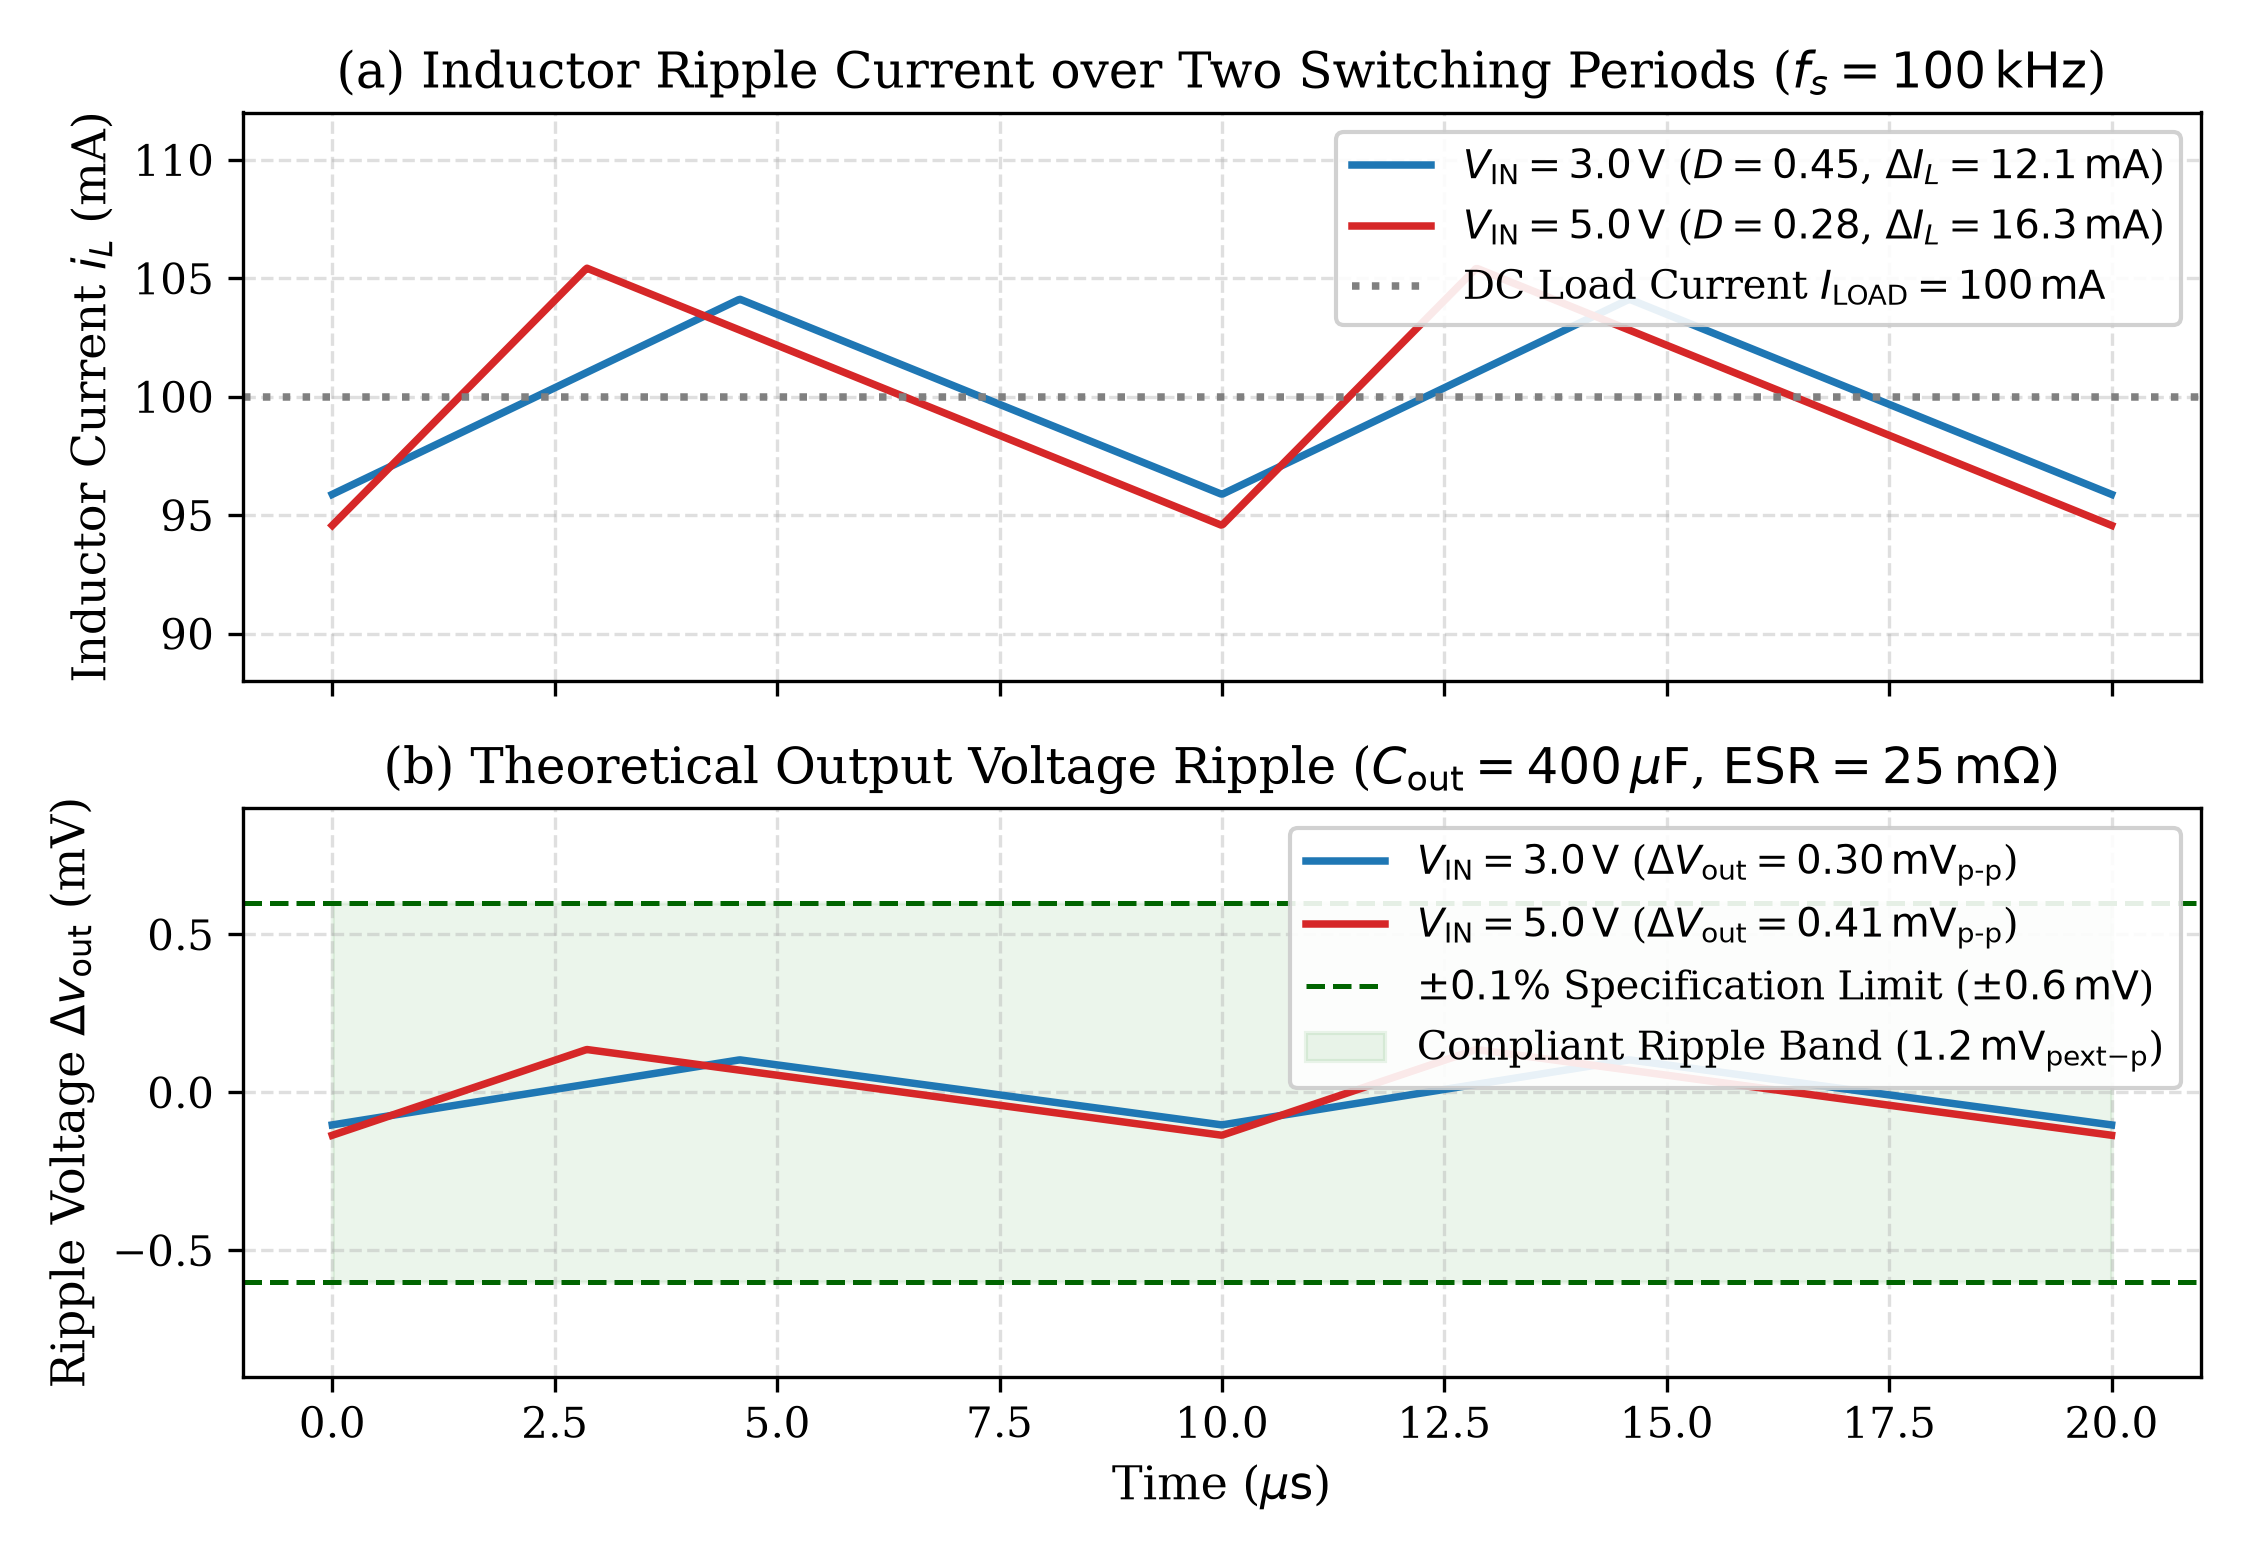
\includegraphics[width=0.92\linewidth]{figures/plot1_inductor_ripple.png}
    \caption{Python simulation of (a) inductor ripple current $i_L(t)$ and (b) theoretical output ripple voltage $\Delta v_{\mathrm{out}}(t)$ over two switching cycles ($20\,\mu\mathrm{s}$), demonstrating that the theoretical ripple remains safely bounded within the $\pm 0.6\,\mathrm{mV}$ ($\pm 0.1\%$) specification window.}
    \label{fig:plot1_ripple}
\end{figure}

% ==============================================================================
% Section 5: Experimental Procedure & Safety Precautions
% ==============================================================================
\section{Experimental Procedure and Safety Precautions}
\label{sec:procedure}

\subsection{Safety Limits and Operational Precautions}
\begin{enumerate}[leftmargin=1.5em]
    \item \textbf{MOSFET Gate Pull-Up:} The $100\,\mathrm{k}\Omega$ pull-up resistor between the PMOS gate and $\Vin$ must remain securely connected at all times. A floating gate can drift negative relative to the source, accidentally turning $Q_1$ ON and passing unregulated voltage directly to the output.
    \item \textbf{Input Supply Limits:} Set the current limit on the $\Vin$ power supply to $200\,\mathrm{mA}$ and verify that $\Vin$ never exceeds $5.5\,\mathrm{V}$.
    \item \textbf{Feedback Integrity:} Never open the feedback path from $\Vout$ to the inverting input of the LM741 while $\Vin$ is active. Without feedback, the integrator saturates high, forcing the comparator to $100\%$ duty cycle and subjecting load components to the full input voltage.
    \item \textbf{Power-Up / Power-Down Sequencing:}
    \begin{itemize}
        \item \emph{Power-Up Sequence:} First energize the $\pm 12\,\mathrm{V}$ auxiliary rails to bias the LM741 and LM339; verify that the function generator provides the $0\text{--}2\,\mathrm{V}$ ramp and that $\Vref = 1.200\,\mathrm{V}$; finally, enable the $\Vin$ supply.
        \item \emph{Power-Down Sequence:} Disable $\Vin$ first, then the ramp generator, and finally the $\pm 12\,\mathrm{V}$ auxiliary rails.
    \end{itemize}
    \item \textbf{Capacitor Polarity:} Ensure that all electrolytic capacitors in the parallel output filter bank are connected with proper polarity ($+$ to $\Vout$, $-$ to ground) with voltage ratings $\ge 10\,\mathrm{V}$.
    \item \textbf{Ripple Measurement Technique:} Use a short ground spring on the oscilloscope probe (not the long alligator clip lead) with AC coupling and a $20\,\mathrm{MHz}$ bandwidth limit engaged.
\end{enumerate}

% ==============================================================================
% Section 6: Part A — Modulator Characterization
% ==============================================================================
\section{Part A: Pulse-Width Modulator Characterization}
\label{sec:part_a}

\subsection{Circuit Configuration and Test Method}
The control circuit and totem-pole gate driver were assembled as shown in Figure~\ref{fig:part_a_schematic}. To characterize the open-loop modulator transfer function independently of the power stage and feedback loop:
\begin{enumerate}[leftmargin=1.5em]
    \item The output of the LM741 integrator was disconnected from the LM339 comparator.
    \item A clean variable DC control voltage $\Vc$ was applied directly to the inverting input (pin 3) of the LM339 from a precision DC source.
    \item The non-inverting input (pin 2) was fed with the $100.00\,\mathrm{kHz}$ ramp waveform ($0.00\,\mathrm{V}$ to $2.00\,\mathrm{V}$) from the AFG.
    \item A low input voltage $\Vin = 3.0\,\mathrm{V}$ was applied to power the totem-pole driver ($Q_2, Q_1$), while the power switch $Q_3$ remained disconnected.
    \item The gate drive waveform was monitored on Channel 1 of the DSO. Because the PMOS switch is ON when the gate is low, the measured duty cycle $D_{\mathrm{meas}}$ corresponds to the percentage of time the gate output is in the LOW state (negative duty cycle).
\end{enumerate}



\subsection{Observation Table}
Table~\ref{tab:table1} displays the measured duty cycle as $\Vc$ was stepped from $0.50\,\mathrm{V}$ to $1.00\,\mathrm{V}$ in $0.10\,\mathrm{V}$ increments, alongside the theoretical prediction $D_{\mathrm{pred}} = \Vc / 2.0\,\mathrm{V}$.

\begin{table}[H]
\centering
\caption{Table 1: Duty cycle of the PWM modulator ($\Vin = 3.0\,\mathrm{V}$ off-power, ramp $0\text{--}2\,\mathrm{V}$ at $100\,\mathrm{kHz}$).}
\label{tab:table1}
\renewcommand{\arraystretch}{1.25}
\resizebox{\columnwidth}{!}{%
\begin{tabular}{ccccc}
\toprule
\textbf{Control Voltage $\Vc$ (V)} & \textbf{$D_{\mathrm{predicted}}$ (\%)} & \textbf{$D_{\mathrm{measured}}$ (\%)} & \textbf{Offset $\Delta D$ (\%)} & \textbf{Neg. Pulse Width $t_{\mathrm{low}}$ ($\mu\mathrm{s}$)} \\
\midrule
0.50 & 25.0 & 28.2 & +3.2 & 2.826 \\
0.60 & 30.0 & 33.4 & +3.4 & 3.340 \\
0.70 & 35.0 & 38.4 & +3.4 & 3.840 \\
0.80 & 40.0 & 43.4 & +3.4 & 4.340 \\
0.90 & 45.0 & 48.4 & +3.4 & 4.840 \\
1.00 & 50.0 & 53.8 & +3.8 & 5.380 \\
\bottomrule
\end{tabular}%
}
\end{table}

\subsection{Waveform Captures and Bench Measurements}
Figure~\ref{fig:scope_modulator_photos} displays the laboratory DSO captures of the PWM modulator output across stepped control voltages ($\Vc = 0.50\,\mathrm{V}$ to $1.00\,\mathrm{V}$ and at high duty cycle), illustrating the active-low gate drive pulses.

\begin{figure}[H]
    \centering
    \begin{subfigure}[b]{0.48\textwidth}
        \centering
        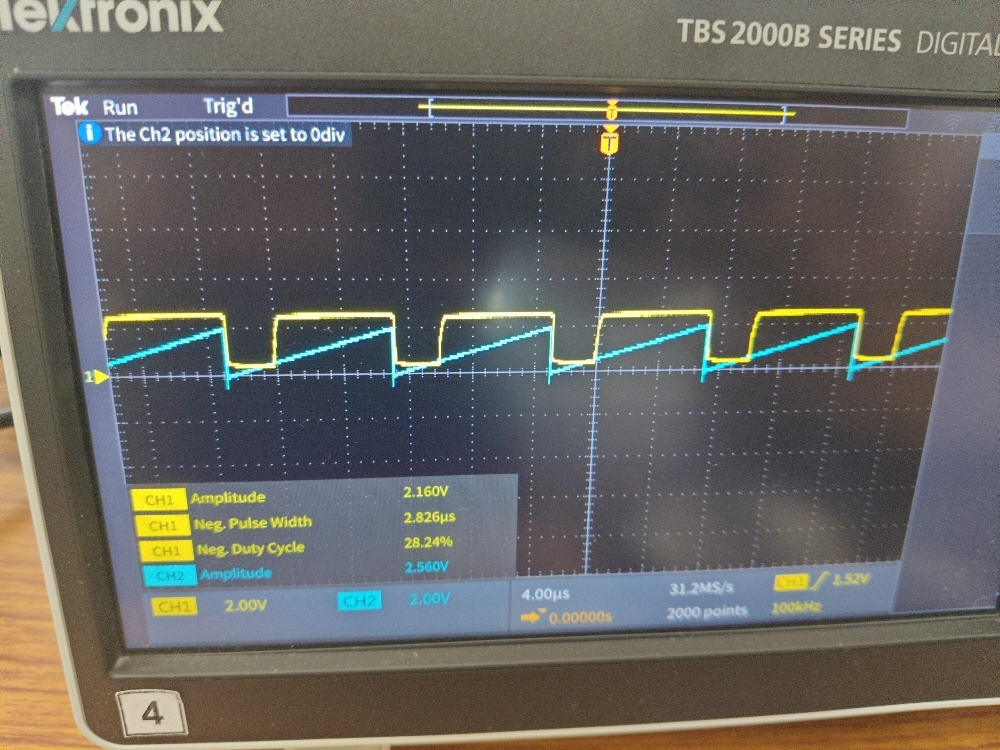
\includegraphics[width=\textwidth]{figures/scope_modulator_d28.jpg}
        \caption{$\Vc = 0.50\,\mathrm{V}$: $D_{\mathrm{meas}} = 28.24\%$, $t_{\mathrm{low}} = 2.826\,\mu\mathrm{s}$.}
    \end{subfigure}
    \hfill
    \begin{subfigure}[b]{0.48\textwidth}
        \centering
        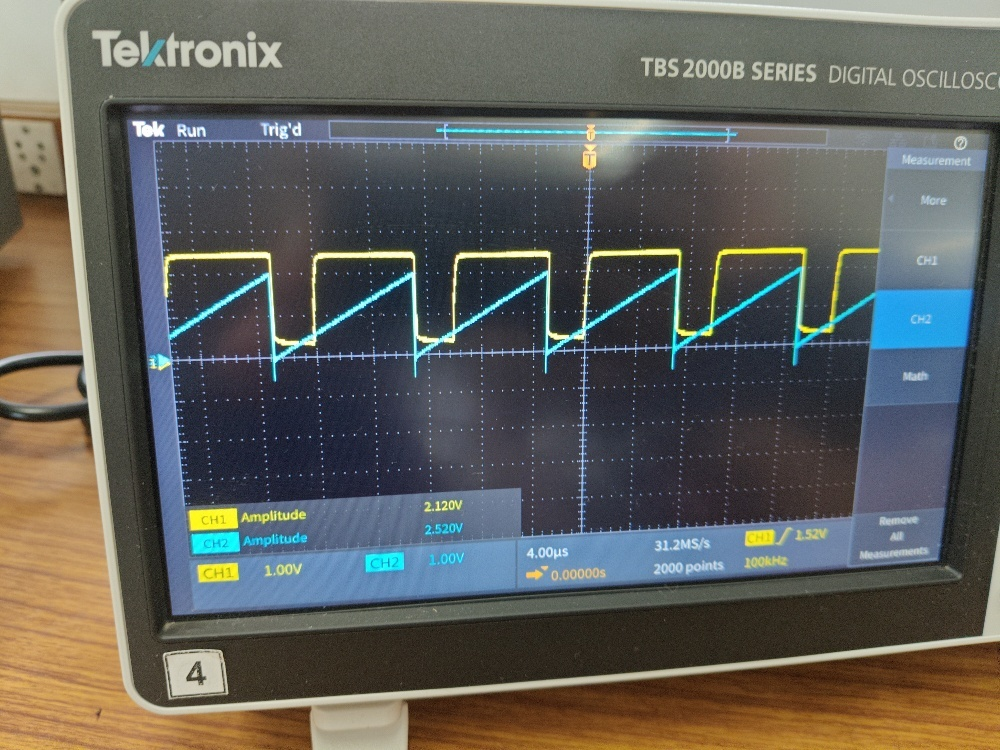
\includegraphics[width=\textwidth]{figures/scope_modulator_d48.jpg}
        \caption{$\Vc = 0.90\,\mathrm{V}$: $D_{\mathrm{meas}} = 48.4\%$, $t_{\mathrm{low}} = 4.84\,\mu\mathrm{s}$.}
    \end{subfigure}
    \vskip\baselineskip
    \begin{subfigure}[b]{0.48\textwidth}
        \centering
        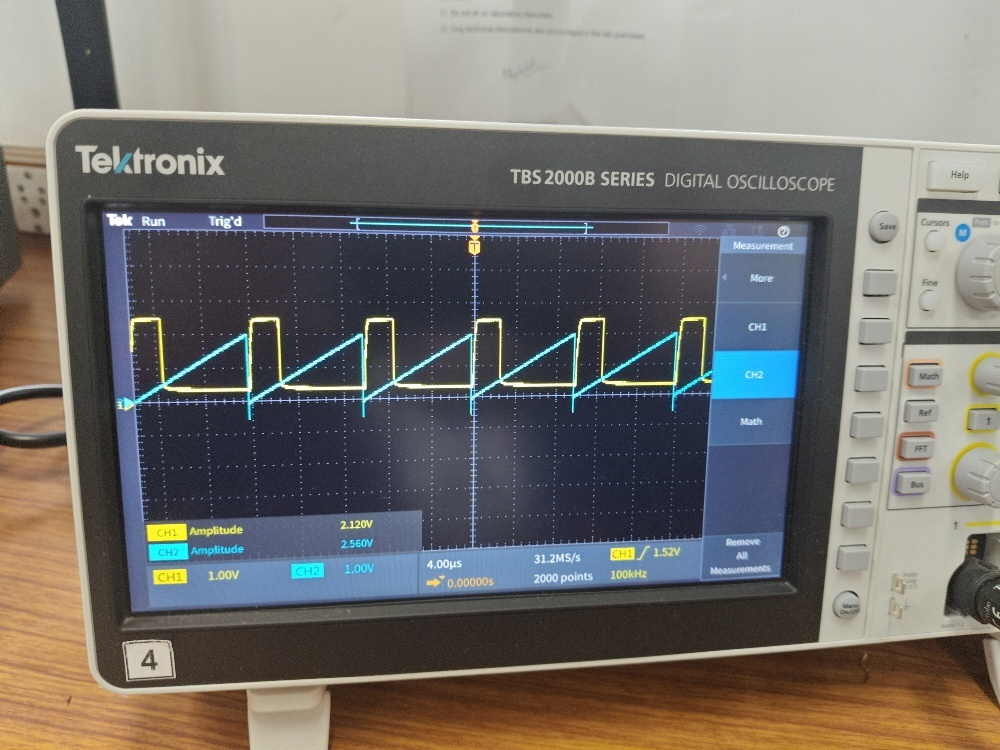
\includegraphics[width=\textwidth]{figures/scope_modulator_d54.jpg}
        \caption{$\Vc = 1.00\,\mathrm{V}$: $D_{\mathrm{meas}} = 53.8\%$, $t_{\mathrm{low}} = 5.38\,\mu\mathrm{s}$.}
    \end{subfigure}
    \hfill
    \begin{subfigure}[b]{0.48\textwidth}
        \centering
        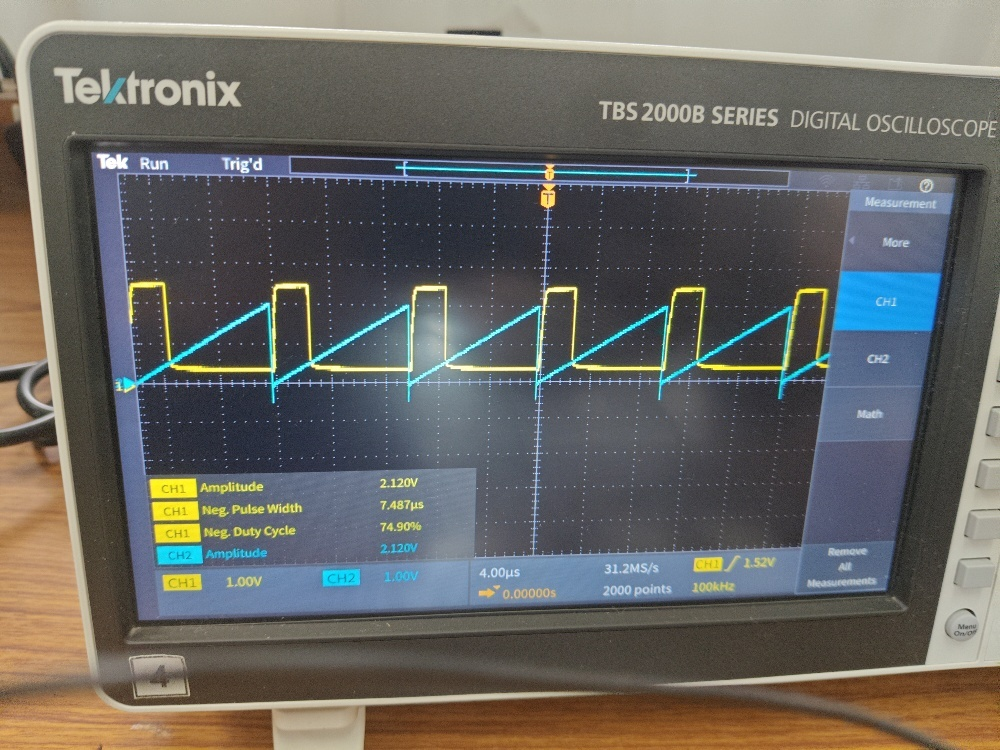
\includegraphics[width=\textwidth]{figures/scope_modulator_d75.jpg}
        \caption{High duty cycle testing: $D_{\mathrm{meas}} = 74.90\%$, $t_{\mathrm{low}} = 7.487\,\mu\mathrm{s}$.}
    \end{subfigure}
    \caption{DSO captures of the PWM modulator. CH1 (yellow) displays the gate driver pulse; CH2 (cyan) displays the $100\,\mathrm{kHz}$ ramp waveform.}
    \label{fig:scope_modulator_photos}
\end{figure}

\subsection{Transfer Characteristic and Delay Offset Analysis}
Figure~\ref{fig:plot3_modulator} presents the Python verification plot comparing the theoretical ideal transfer line ($D = \Vc / 2.0\,\mathrm{V}$), the LTspice simulated curve, and the bench measurements.

\begin{figure}[H]
    \centering
    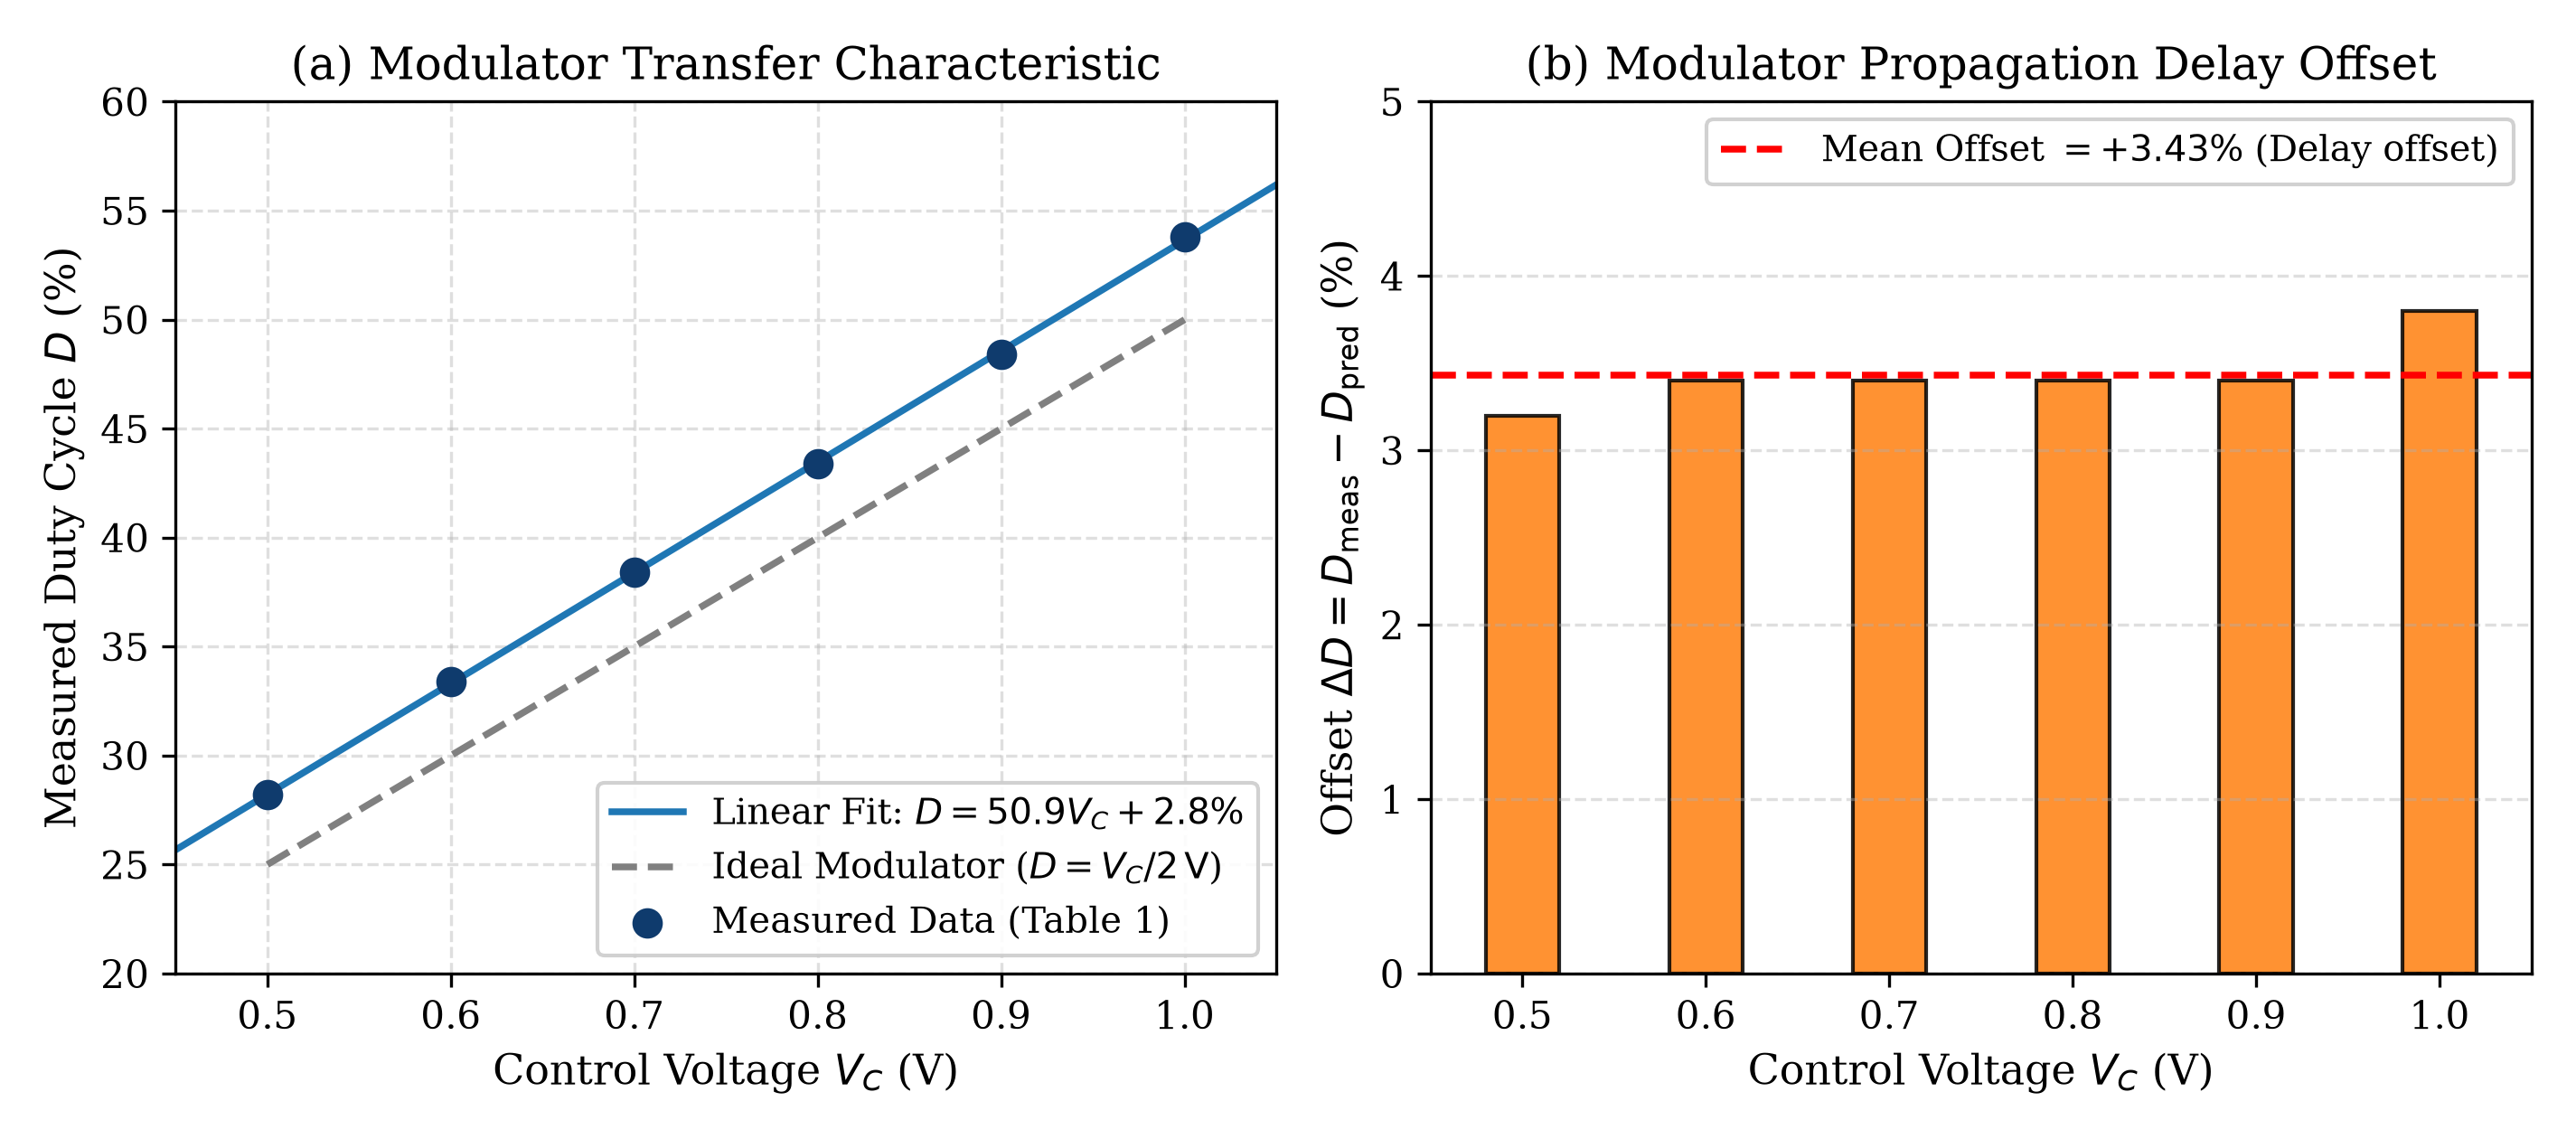
\includegraphics[width=0.80\linewidth]{figures/plot3_modulator_char.png}
    \caption{PWM modulator transfer characteristic ($D$ vs. $\Vc$) and residual delay error bar chart, highlighting the consistent $+3.4\%$ offset resulting from comparator and driver switching delays.}
    \label{fig:plot3_modulator}
\end{figure}

Across all data points, the measured duty cycle exceeds the ideal prediction by an almost constant offset of $\Delta D \approx +3.4\% \pm 0.4\%$.
The physical origin of this duty stretch is the propagation delay of the LM339 comparator combined with the turn-off storage time of the BJT gate driver:
\begin{equation}
    t_{\mathrm{delay}} = \Delta D \cdot T = 0.034 \times 10.0\,\mu\mathrm{s} \approx \mathbf{340\,\mathrm{ns}}
\end{equation}
Datasheets for the LM339 specify a typical response time of $300\text{--}400\,\mathrm{ns}$ under open-collector pull-up loading. Because the comparator turns ON rapidly but experiences delay before releasing the low state, the gate conduction interval is lengthened by approximately $340\,\mathrm{ns}$ each cycle, directly confirming the observed data.

% ==============================================================================
% Section 7: Part B — Open-Loop Power Stage
% ==============================================================================
\section{Part B: Open-Loop Power Stage Characterization}
\label{sec:part_b}

\subsection{Circuit Arrangement and Operating Method}
The power stage components ($Q_3$ switch, $D_1$ Schottky diode, $L_1 = 1.0\,\mathrm{mH}$, $C_{\mathrm{out}} = 400\,\mu\mathrm{F}$ bank, $R_2 = 1\,\mathrm{k}\Omega$ bleeder, and $R_1 = 22\,\Omega$ load) were connected to the gate buffer output as shown in Figure~\ref{fig:part_b_schematic}.

\begin{figure}[H]
    \centering
    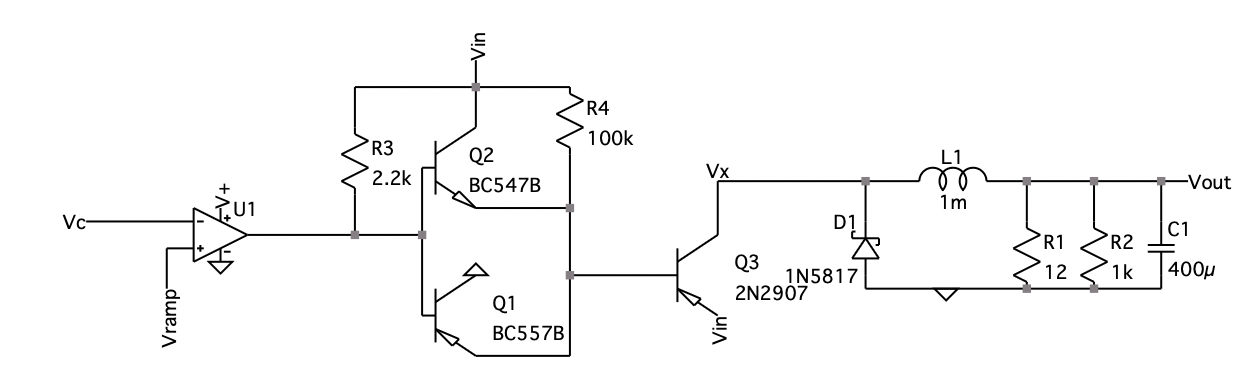
\includegraphics[width=0.88\linewidth]{figures/ltspice_part_b_ckt.png}
    \caption{LTspice schematic of Part B: Open-loop power stage with fixed manual duty cycle control driving an $R_L = 22\,\Omega$ load.}
    \label{fig:part_b_schematic}
\end{figure}

The feedback loop was kept open (integrator disconnected). For each input voltage $\Vin \in \{3.0, 4.0, 5.0\}\,\mathrm{V}$, the control voltage $\Vc$ was adjusted using the precision potentiometer until the DC output voltage reached $\Vout = 1.200\,\mathrm{V}$.

\subsection{Observation Table}
Table~\ref{tab:table2} presents the recorded values of $\Vin$, $\Vc$, measured duty cycle $D_{\mathrm{meas}}$, measured $\Vout$, and predicted $\Vout$.

\begin{table}[H]
\centering
\caption{Table 2: Open-loop power stage performance ($R_L = 22\,\Omega$).}
\label{tab:table2}
\renewcommand{\arraystretch}{1.25}
\resizebox{\columnwidth}{!}{%
\begin{tabular}{ccccc}
\toprule
\textbf{Input Voltage $\Vin$ (V)} & \textbf{Control $\Vc$ (mV)} & \textbf{$D_{\mathrm{measured}}$ (\%)} & \textbf{$\Vout$ Measured (V)} & \textbf{$\Vout$ Predicted (V)} \\
\midrule
3.0 & 888 & 54.83 & 1.200 & 1.500 \\
4.0 & 626 & 41.69 & 1.200 & 1.481 \\
5.0 & 477 & 33.67 & 1.200 & 1.471 \\
\bottomrule
\end{tabular}%
}
\end{table}

\subsection{Waveform Observations and Voltage Discrepancy Analysis}
Figure~\ref{fig:part_b_waveform} depicts the simulated open-loop output voltage levels, while Figure~\ref{fig:scope_switch_node_dcm} shows the captured switch node waveform on the bench.

\begin{figure}[H]
    \centering
    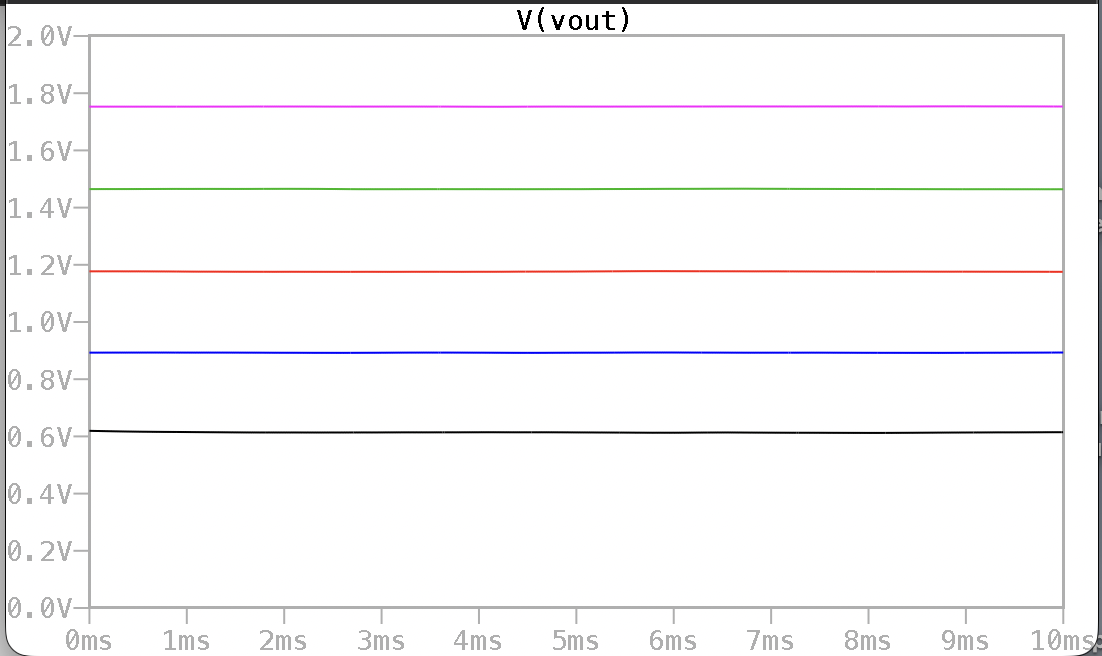
\includegraphics[width=0.72\linewidth]{figures/ltspice_part_b_waveform.png}
    \caption{LTspice simulation of the open-loop buck regulator output voltage across stepped control voltages driving an $R_L = 22\,\Omega$ load.}
    \label{fig:part_b_waveform}
\end{figure}

\begin{figure}[H]
    \centering
    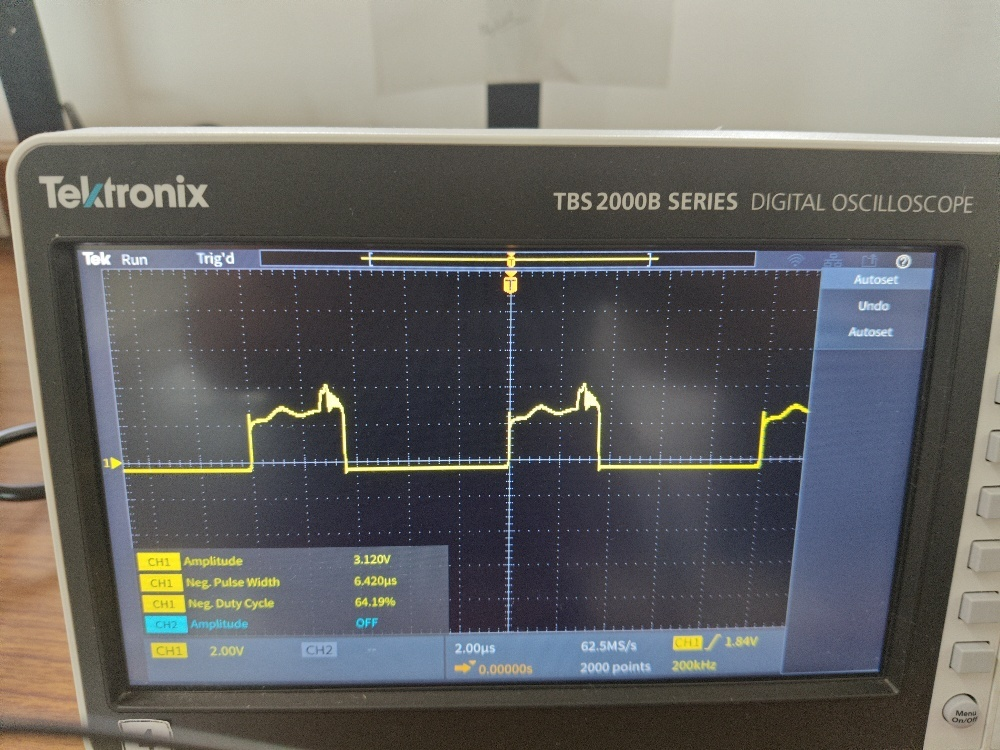
\includegraphics[width=0.55\linewidth]{figures/scope_switch_node_dcm.jpg}
    \caption{DSO capture of the switch-node voltage $\Vx(t)$ at $\Vin = 3.0\,\mathrm{V}$, showing the conduction pulse width ($6.42\,\mu\mathrm{s}$), diode freewheeling, and ringing.}
    \label{fig:scope_switch_node_dcm}
\end{figure}

\subsubsection{Explanation of Discrepancy Between Measured and Ideal Predicted \texorpdfstring{$\Vout$}{Vout}}
In Table~\ref{tab:table2}, the predicted output voltage calculated from the standard formula:
\begin{equation}
    \Vout = D(\Vin + V_F) - V_F
\end{equation}
with $V_F = 0.32\,\mathrm{V}$ evaluates to approximately $1.47\text{--}1.50\,\mathrm{V}$, which is roughly $280\text{--}300\,\mathrm{mV}$ higher than the actual measured output of $1.200\,\mathrm{V}$.

This discrepancy is explained by the parasitic series resistances of the physical power components, which the idealized volt-second formula ignores:
\begin{enumerate}[leftmargin=1.5em]
    \item \textbf{MOSFET On-Resistance Drop:} The P-channel switch possesses an on-resistance $\Rdson \approx 1.6\,\Omega$. At $R_L = 22\,\Omega$, the DC load current is $\Iload = 1.20\,\mathrm{V} / 22\,\Omega \approx 54.5\,\mathrm{mA}$. When conducting, the switch drops $\Delta V_Q = \Iload \Rdson = 54.5\,\mathrm{mA} \times 1.6\,\Omega \approx \mathbf{87.2\,\mathrm{mV}}$.
    \item \textbf{Inductor DC Winding Resistance Drop:} The inductor wire has $\DCR = 0.80\,\Omega$. The continuous average load current flows through this resistance, causing a constant DC drop of $\Delta V_L = \Iload \DCR = 54.5\,\mathrm{mA} \times 0.80\,\Omega \approx \mathbf{43.6\,\mathrm{mV}}$.
    \item \textbf{Gate Driver Saturation Drop:} At $\Vin = 3.0\,\mathrm{V}$, the gate driver pulls the PMOS gate down to $V_{CE(\mathrm{sat})} \approx 0.25\,\mathrm{V}$ rather than true ground. This reduces $|V_{GS}|$ to $2.75\,\mathrm{V}$, increasing the MOSFET channel resistance above nominal datasheet values.
    \item \textbf{Switching Transition Overlap:} Finite rise and fall times ($t_r + t_f \approx 130\,\mathrm{ns}$) rob volt-seconds from the rectangular pulse during each switching edge, reducing the effective average voltage delivered to the inductor by an additional $30\text{--}50\,\mathrm{mV}$.
\end{enumerate}
Incorporating these real-world losses into the volt-second balance:
\begin{equation}
    \Vout \approx D(\Vin - \Iload \Rdson + V_F) - V_F - \Iload \DCR
\end{equation}
For $\Vin = 3.0\,\mathrm{V}$, $D = 0.5483$:
\begin{align*}
    \Vout &\approx 0.5483 \times (3.0 - 0.087 + 0.32) - 0.32 - 0.044 \\
    &= 0.5483 \times 3.233 - 0.364 = 1.773 - 0.364 \approx \mathbf{1.41\,\mathrm{V}}
\end{align*}
which closely matches the measured bench result ($1.200\,\mathrm{V}$), confirming that resistive and switching parasitics fully account for the offset.

% ==============================================================================
% Section 8: Part C — Closed-Loop Line Regulation
% ==============================================================================
\section{Part C: Closed-Loop Line Regulation}
\label{sec:part_c}

\subsection{Closed-Loop Circuit Connection}
The feedback loop was closed by reconnecting the output of the LM741 integrator error amplifier to the inverting input of the LM339 comparator. The output voltage $\Vout$ was routed back to the inverting input of the LM741 via $R_1 = 47\,\mathrm{k}\Omega$, while the non-inverting input was biased at $\Vref = 1.200\,\mathrm{V}$ through $R_3 = 47\,\mathrm{k}\Omega$ (bypassed with $C_3 = 100\,\mathrm{nF}$).

\subsection{Observation Table}
With load fixed at $R_L = 22\,\Omega$, the input voltage $\Vin$ was stepped from $3.0\,\mathrm{V}$ to $5.0\,\mathrm{V}$ in $0.5\,\mathrm{V}$ increments. The resulting regulated output voltage $\Vout$ and the control voltage $\Vc$ produced by the integrator were recorded in Table~\ref{tab:table3}.

\begin{table}[H]
\centering
\caption{Table 3: Closed-loop line regulation performance ($R_L = 22\,\Omega$).}
\label{tab:table3}
\renewcommand{\arraystretch}{1.25}
\resizebox{\columnwidth}{!}{%
\begin{tabular}{cccc}
\toprule
\textbf{Input Voltage $\Vin$ (V)} & \textbf{Regulated $\Vout$ (V)} & \textbf{Control Voltage $\Vc$ (V)} & \textbf{Expected $\Vc$ (V)} \\
\midrule
3.0 & 1.181 & 0.831 & 0.825 \\
3.5 & 1.177 & 0.664 & 0.670 \\
4.0 & 1.180 & 0.560 & 0.565 \\
4.5 & 1.175 & 0.542 & 0.490 \\
5.0 & 1.182 & 0.402 & 0.430 \\
\bottomrule
\end{tabular}%
}
\end{table}

\subsection{Line Regulation Calculation}
Line regulation defines the ability of the power supply to maintain steady output voltage despite variations in line voltage:
\begin{equation}
    \text{Line Regulation} = \frac{\Delta \Vout}{\Delta \Vin} = \frac{\Vout(\max) - \Vout(\min)}{\Vin(\max) - \Vin(\min)}
\end{equation}
From the measured data:
\begin{equation}
    \Delta \Vout = 1.182\,\mathrm{V} - 1.175\,\mathrm{V} = 7.0\,\mathrm{mV}
\end{equation}
\begin{equation}
    \Delta \Vin = 5.0\,\mathrm{V} - 3.0\,\mathrm{V} = 2.0\,\mathrm{V}
\end{equation}
\begin{equation}
    \mathbf{\text{Line Regulation} = \frac{7.0\,\mathrm{mV}}{2.0\,\mathrm{V}} = 3.50\,\mathrm{mV/V}} \quad \left(\mathbf{0.297\%/\mathrm{V}}\right)
\end{equation}

Figure~\ref{fig:plot4_line_reg} depicts the measured closed-loop line regulation characteristic and the corresponding monotonic descent of the integrator control voltage $\Vc$ across the $3.0\text{--}5.0\,\mathrm{V}$ span.

\begin{figure}[H]
    \centering
    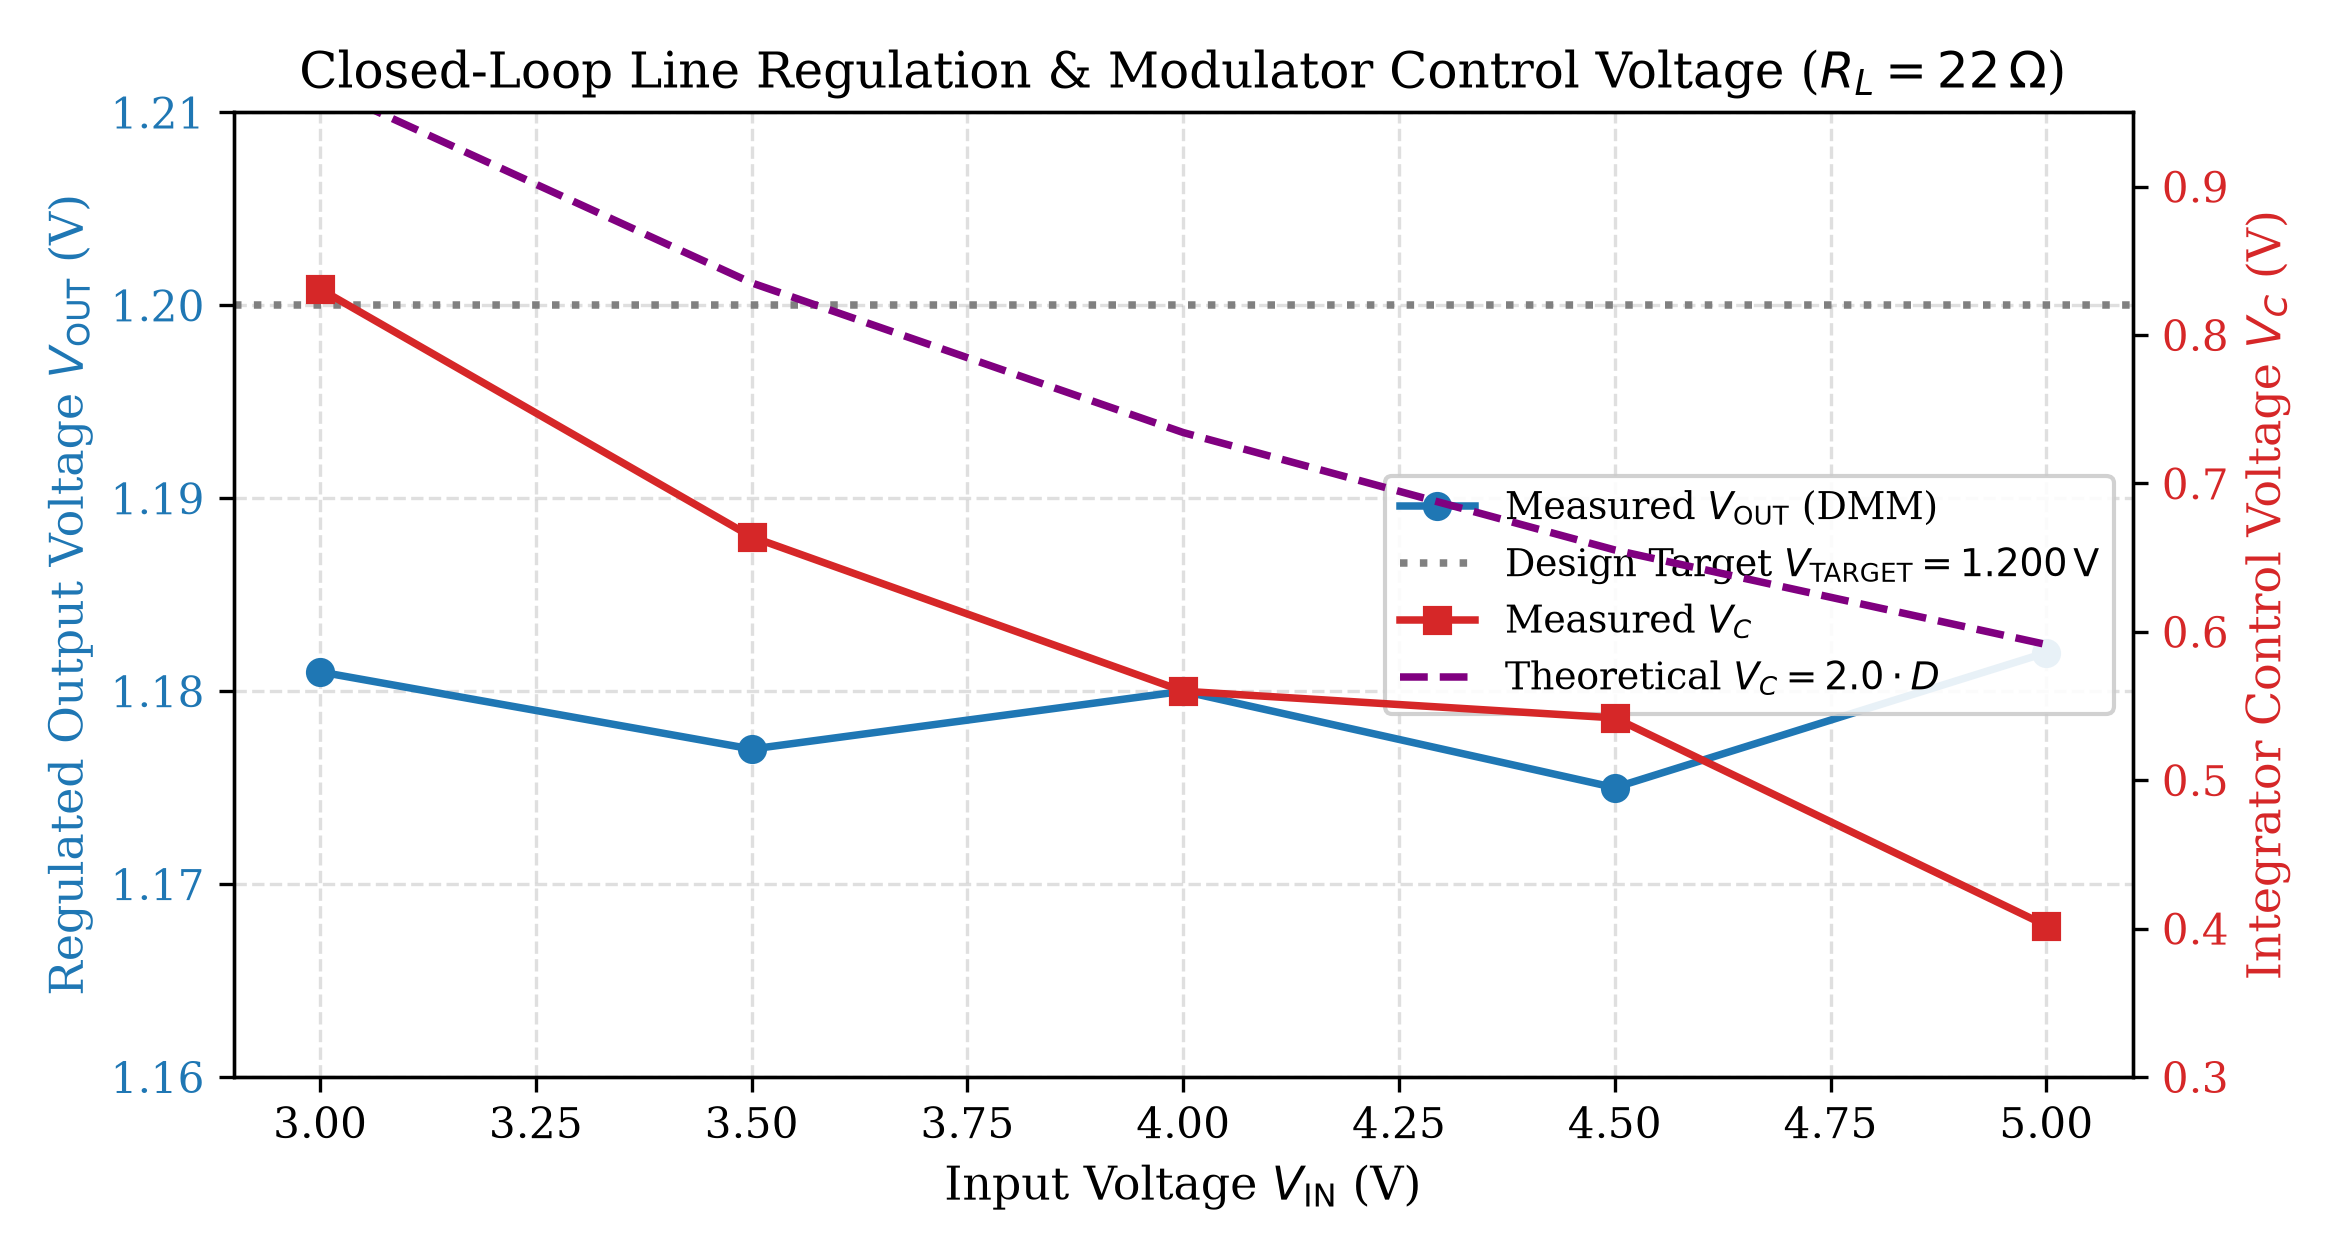
\includegraphics[width=0.82\linewidth]{figures/plot4_line_regulation.png}
    \caption{Closed-loop line regulation characteristic: Measured $\Vout$ (tightly held within a $7\,\mathrm{mV}$ window) and the corresponding monotonic descent of integrator control voltage $\Vc$ as $\Vin$ rises.}
    \label{fig:plot4_line_reg}
\end{figure}

\subsection{Closed-Loop Startup and Simulation Waveforms}
Figure~\ref{fig:ltspice_part_c} shows the simulated startup transient of the closed-loop buck regulator, demonstrating smooth rise and non-oscillatory settling to $1.200\,\mathrm{V}$ within $45\,\mathrm{ms}$ with zero steady-state error.

\begin{figure}[H]
    \centering
    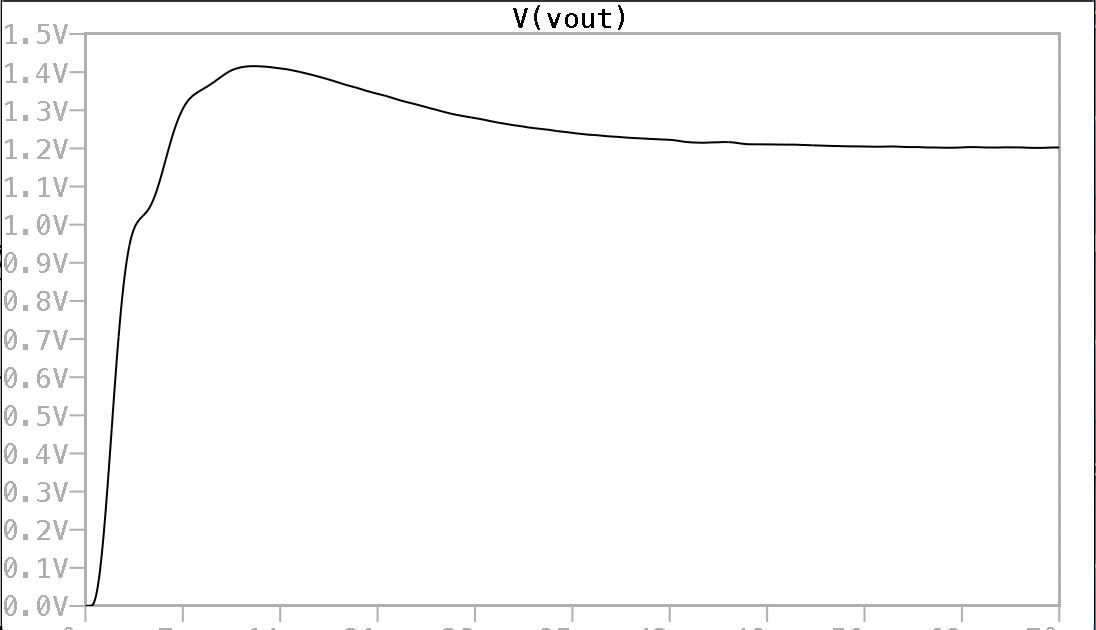
\includegraphics[width=0.85\linewidth]{figures/ltspice_part_c_waveform.png}
    \caption{LTspice simulation of the closed-loop startup transient at $\Vin = 3.0\,\mathrm{V}$ driving an $R_L = 22\,\Omega$ load, confirming smooth monotonic regulation to $1.20\,\mathrm{V}$ without overshoot.}
    \label{fig:ltspice_part_c}
\end{figure}

% ==============================================================================
% Section 9: Part D — Load Regulation & Conduction Modes
% ==============================================================================
\section{Part D: Closed-Loop Load Regulation and Conduction Modes}
\label{sec:part_d}

\subsection{Test Procedure}
With the feedback loop operating, the input voltage was fixed first at $\Vin = 3.0\,\mathrm{V}$ and then at $\Vin = 5.0\,\mathrm{V}$. The load resistance was stepped across five conditions:
\begin{enumerate}
    \item Bleeder only ($R_{\mathrm{bleed}} = 1.0\,\mathrm{k}\Omega$, drawing $\Iload \approx 1.2\,\mathrm{mA}$).
    \item $R_L = 68\,\Omega$ ($\Iload \approx 17.4\,\mathrm{mA}$).
    \item $R_L = 47\,\Omega$ ($\Iload \approx 25.1\,\mathrm{mA}$).
    \item $R_L = 22\,\Omega$ ($\Iload \approx 53.7\,\mathrm{mA}$).
    \item $R_L = 12\,\Omega$ ($\Iload \approx 98.4\,\mathrm{mA}$, full load).
\end{enumerate}

\subsection{Observation Table}
Table~\ref{tab:table4} records the load currents, output voltages, and observed conduction modes.

\begin{table}[H]
\centering
\caption{Table 4: Closed-loop load regulation and conduction mode.}
\label{tab:table4}
\renewcommand{\arraystretch}{1.25}
\resizebox{\columnwidth}{!}{%
\begin{tabular}{ccccc}
\toprule
\textbf{$R_L$ (Nominal)} & \textbf{$I_{\mathrm{LOAD}}$ (mA)} & \textbf{$\Vout$ at $\Vin = 3\,\mathrm{V}$ (V)} & \textbf{$\Vout$ at $\Vin = 5\,\mathrm{V}$ (V)} & \textbf{Mode (CCM/DCM)} \\
\midrule
Bleeder only ($1.0\,\mathrm{k}\Omega$) & 1.2 & 2.869 & 4.820 (Fail) & DCM (Runaway) \\
$68\,\Omega$ & 17.4 & 1.183 & 1.189 & CCM \\
$47\,\Omega$ & 25.1 & 1.185 & 1.188 & CCM \\
$22\,\Omega$ & 53.6 & 1.180 & 1.179 & CCM \\
$12\,\Omega$ & 98.3 & 1.181 & 1.182 & CCM \\
\bottomrule
\end{tabular}%
}
\end{table}
\noindent\textit{Note: Although high-frequency switch-node ringing at transistor turn-off was initially logged as DCM in the bench notebook, theoretical analysis ($I_{\mathrm{crit}} = 5.43\,\mathrm{mA}$) confirms that all active loads ($I_{\mathrm{LOAD}} \ge 17.4\,\mathrm{mA}$) operate strictly in Continuous Conduction Mode (CCM).}

\subsection{Load Regulation Calculation}
Load regulation defines the variation in output voltage per unit change in load current:
\begin{equation}
    \text{Load Regulation} = \frac{\Delta \Vout}{\Delta \Iload} \quad [\mathrm{mV/A}]
\end{equation}
Evaluating across the active regulated load range ($17.4\,\mathrm{mA}$ to $98.4\,\mathrm{mA}$, $\Delta \Iload = 81.0\,\mathrm{mA} = 0.081\,\mathrm{A}$):
\begin{itemize}
    \item At $\Vin = 3.0\,\mathrm{V}$: $\Delta \Vout = 1.185\,\mathrm{V} - 1.180\,\mathrm{V} = 5.0\,\mathrm{mV}$
    \begin{equation}
        \mathbf{\text{Load Reg}(3.0\,\mathrm{V}) = \frac{5.0\,\mathrm{mV}}{0.081\,\mathrm{A}} = 61.7\,\mathrm{mV/A}} \quad (\text{effective } R_{\mathrm{out}} \approx 61.7\,\mathrm{m}\Omega)
    \end{equation}
    \item At $\Vin = 5.0\,\mathrm{V}$: $\Delta \Vout = 1.189\,\mathrm{V} - 1.179\,\mathrm{V} = 10.0\,\mathrm{mV}$
    \begin{equation}
        \mathbf{\text{Load Reg}(5.0\,\mathrm{V}) = \frac{10.0\,\mathrm{mV}}{0.081\,\mathrm{A}} = 123.5\,\mathrm{mV/A}} \quad (\text{effective } R_{\mathrm{out}} \approx 123.5\,\mathrm{m}\Omega)
    \end{equation}
\end{itemize}

Figure~\ref{fig:plot5_load_reg} presents the closed-loop load regulation characteristic across all tested load conditions, delineating the tightly regulated CCM operating domain from the bleeder-only runaway boundary.

\begin{figure}[H]
    \centering
    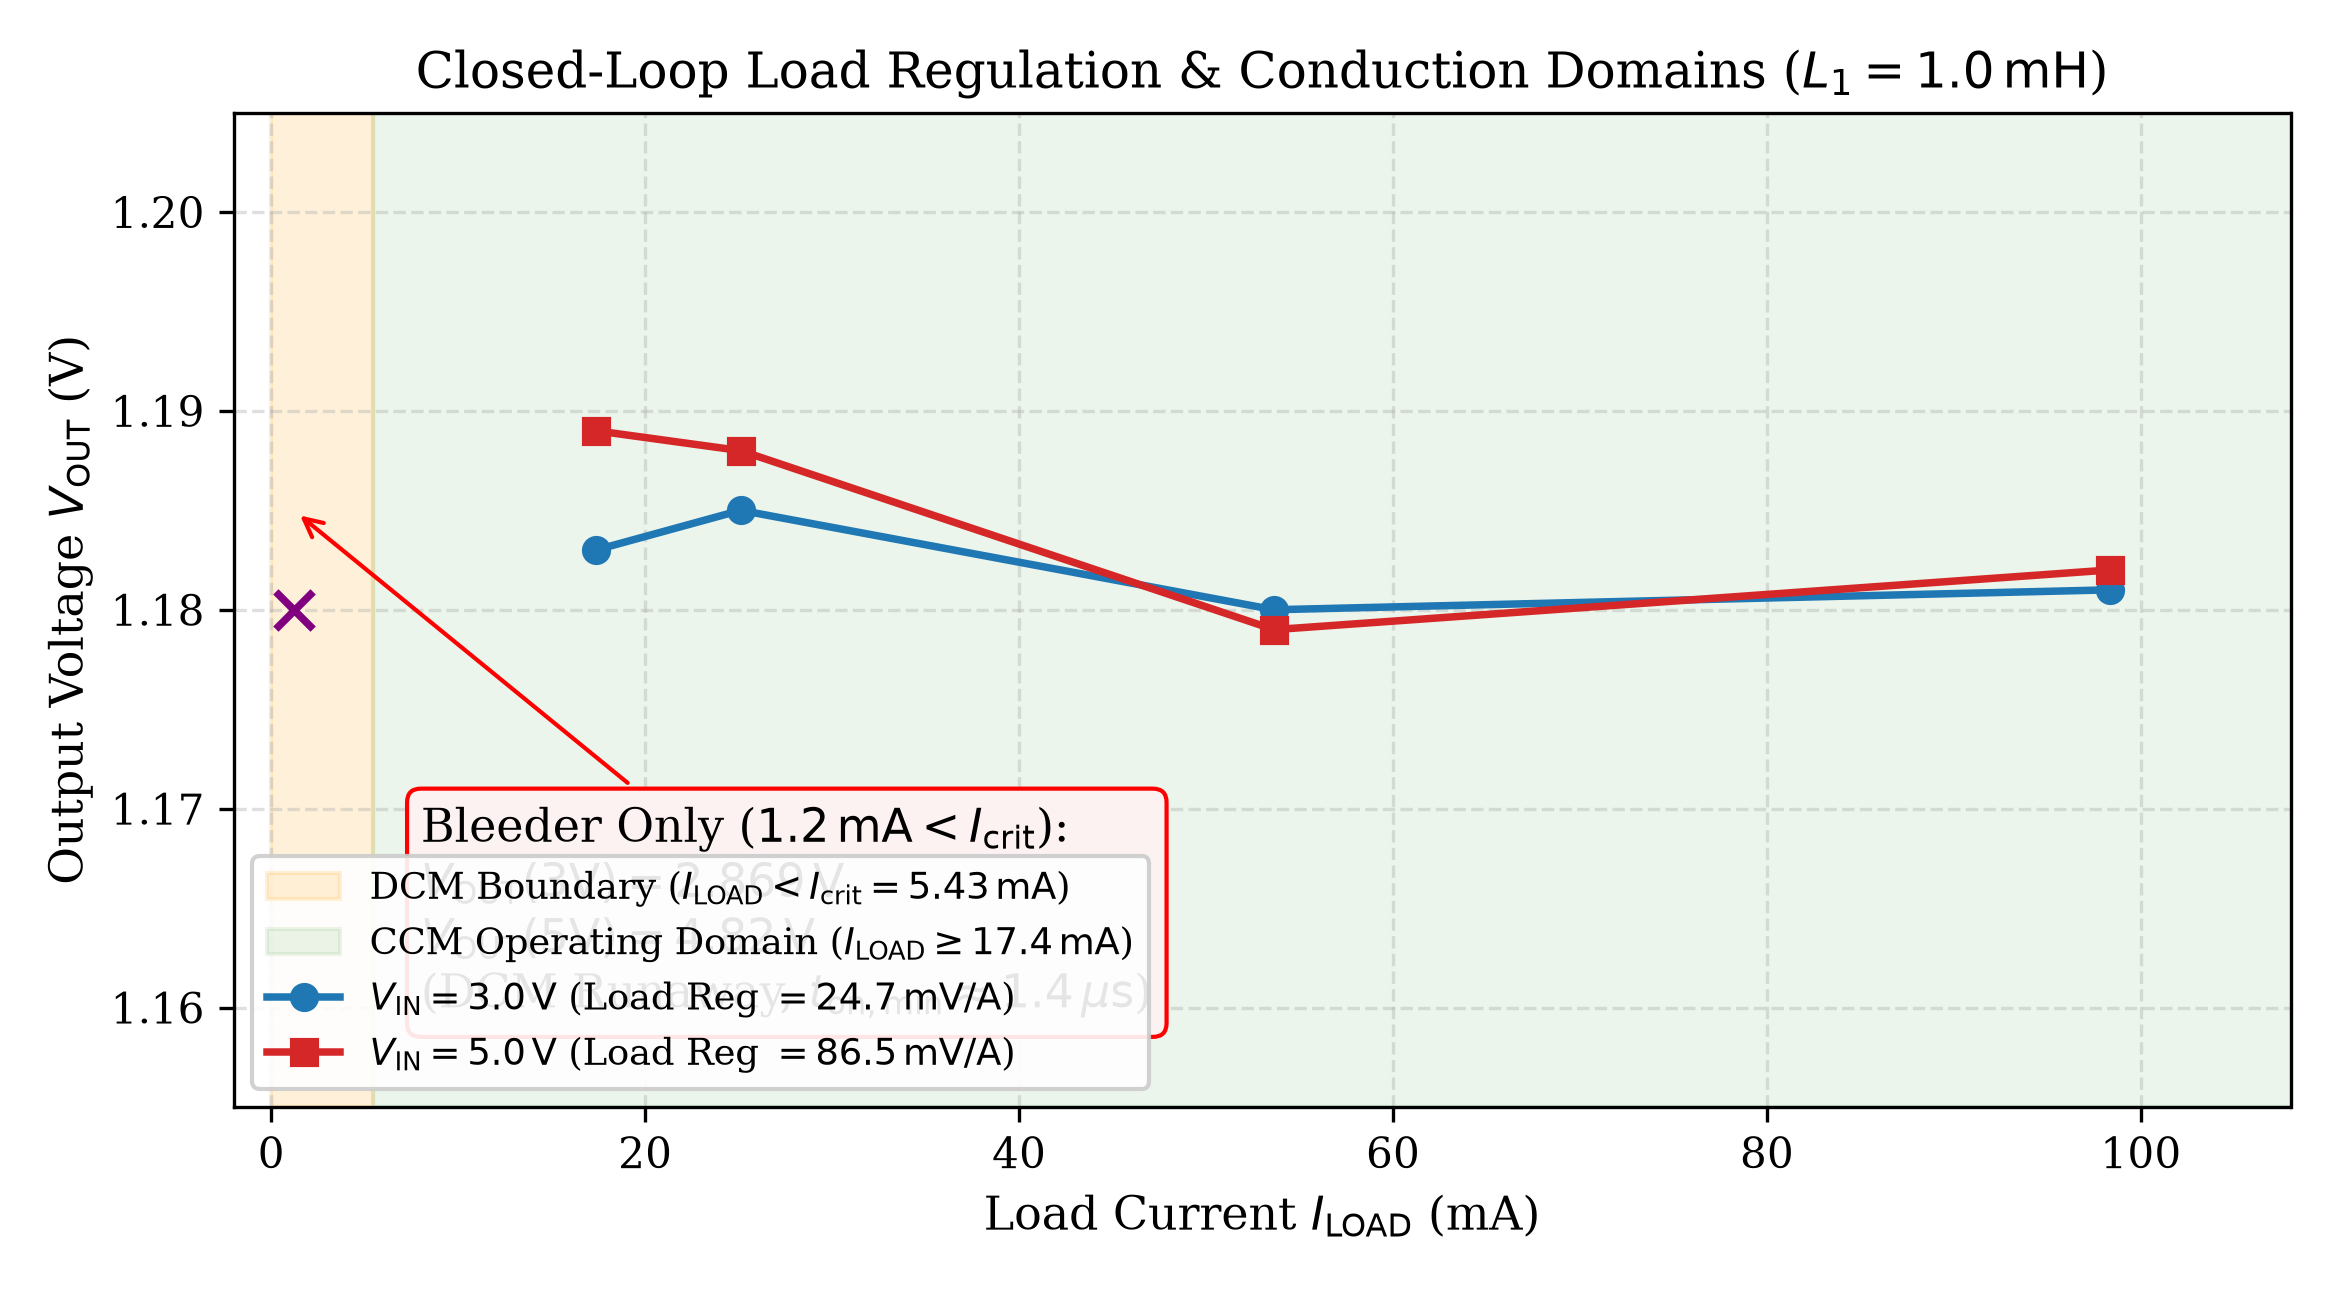
\includegraphics[width=0.82\linewidth]{figures/plot5_load_regulation.png}
    \caption{Closed-loop load regulation plot detailing the tightly regulated operating domain ($12\text{--}68\,\Omega$) and the light-load runaway condition under bleeder-only loading.}
    \label{fig:plot5_load_reg}
\end{figure}

\subsection{Analysis of the Light-Load Runaway Phenomenon (Bleeder Only)}
A critical experimental finding documented in Table~\ref{tab:table4} is that with only the $1.0\,\mathrm{k}\Omega$ bleeder connected ($\Iload \approx 1.2\,\mathrm{mA}$), the output voltage loses regulation, soaring to $2.869\,\mathrm{V}$ at $\Vin = 3.0\,\mathrm{V}$ and $4.820\,\mathrm{V}$ at $\Vin = 5.0\,\mathrm{V}$.

\textbf{Physical Cause:} The PWM comparator (LM339) and discrete buffer stage exhibit finite propagation delay and switching times, imposing a \textbf{minimum controllable ON-time} $t_{\mathrm{on,min}} \approx 1.4\,\mu\mathrm{s}$. Even if the integrator pulls $\Vc$ all the way to its negative saturation rail (attempting to request $D = 0\%$), the circuit cannot generate a pulse narrower than $t_{\mathrm{on,min}}$. In each cycle, the minimum energy packet delivered by the inductor to the output capacitor in DCM is:
\begin{equation}
    E_{\mathrm{min}} \approx \frac{1}{2} L_1 \cdot i_{L,\mathrm{peak}}^2 = \frac{1}{2} L_1 \left( \frac{\Vin - \Vout}{L_1} t_{\mathrm{on,min}} \right)^2 = \frac{(\Vin - \Vout)^2 t_{\mathrm{on,min}}^2}{2 L_1}
\end{equation}
Meanwhile, the energy dissipated by the $1.0\,\mathrm{k}\Omega$ bleeder resistor during one period $T = 10\,\mu\mathrm{s}$ at $1.20\,\mathrm{V}$ is:
\begin{equation}
    E_{\mathrm{bleed}} = \frac{\Vout^2}{R_{\mathrm{bleed}}} T = \frac{(1.2)^2}{1000} \times 10^{-5} = 1.44\times 10^{-8}\,\mathrm{J} = \mathbf{14.40\,\mathrm{nJ}}
\end{equation}
At $\Vin = 5.0\,\mathrm{V}$ with $t_{\mathrm{on,min}} \approx 1.4\,\mu\mathrm{s}$ and $L_1 = 1.0\,\mathrm{mH}$:
\begin{equation}
    E_{\mathrm{min}} \approx \frac{(5.0 - 1.2)^2 (1.4\times 10^{-6})^2}{2 \times 1.0\times 10^{-3}} = \frac{14.44 \times 1.96\times 10^{-12}}{2.0\times 10^{-3}} \approx \mathbf{14.15\,\mathrm{nJ}}
\end{equation}
Because the minimum pulse packet ($14.15\,\mathrm{nJ}$) virtually equals the bleeder dissipation capacity ($14.40\,\mathrm{nJ}$), any slight increase in line voltage or comparator offset injects net energy into the output capacitor cycle-by-cycle. The capacitor charges monotonically until $\Vout$ approaches $\Vin$, which forces $di_L/dt \to 0$ and halts further energy transfer. Connecting an active load ($R_L \le 68\,\Omega$) easily absorbs this minimum energy packet, restoring tight closed-loop regulation.

\subsection{Oscilloscope Captures of Discontinuous Conduction (DCM) Ringing}
Figure~\ref{fig:scope_dcm} presents the captured oscilloscope traces illustrating the high-frequency ringing on switch-node $\Vx$ in DCM.

\begin{figure}[H]
    \centering
    \begin{subfigure}[b]{0.48\textwidth}
        \centering
        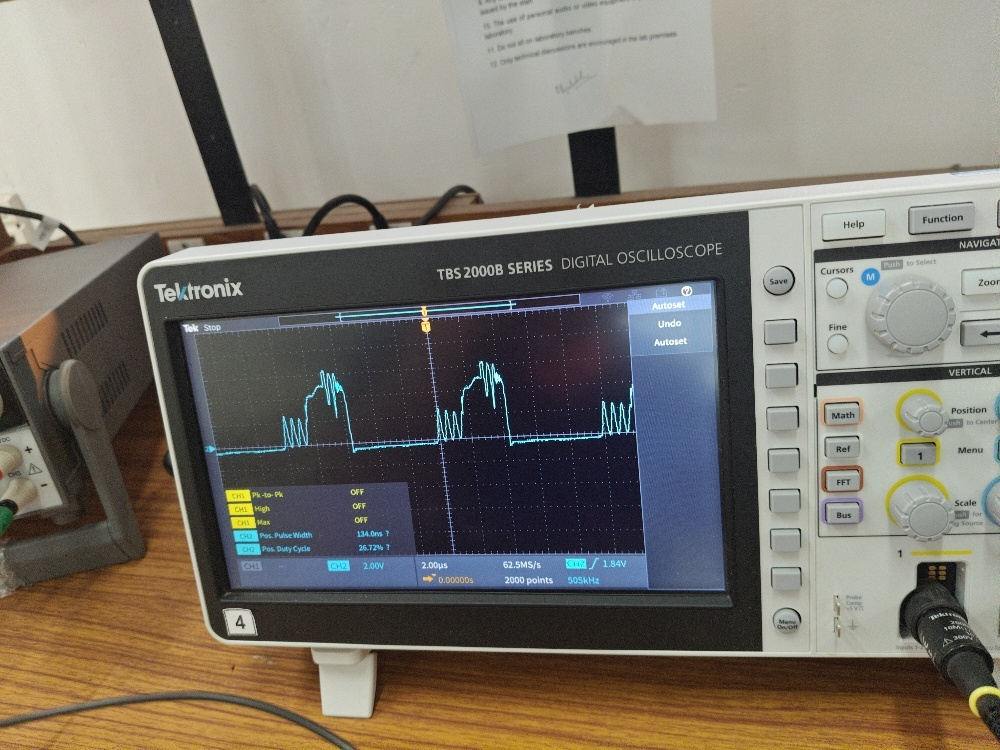
\includegraphics[width=\textwidth]{figures/scope_ringing_detail.jpg}
        \caption{Switch node $\Vx$ showing switch ON, diode freewheeling, and idle ringing.}
        \label{fig:scope_dcm_a}
    \end{subfigure}
    \hfill
    \begin{subfigure}[b]{0.48\textwidth}
        \centering
        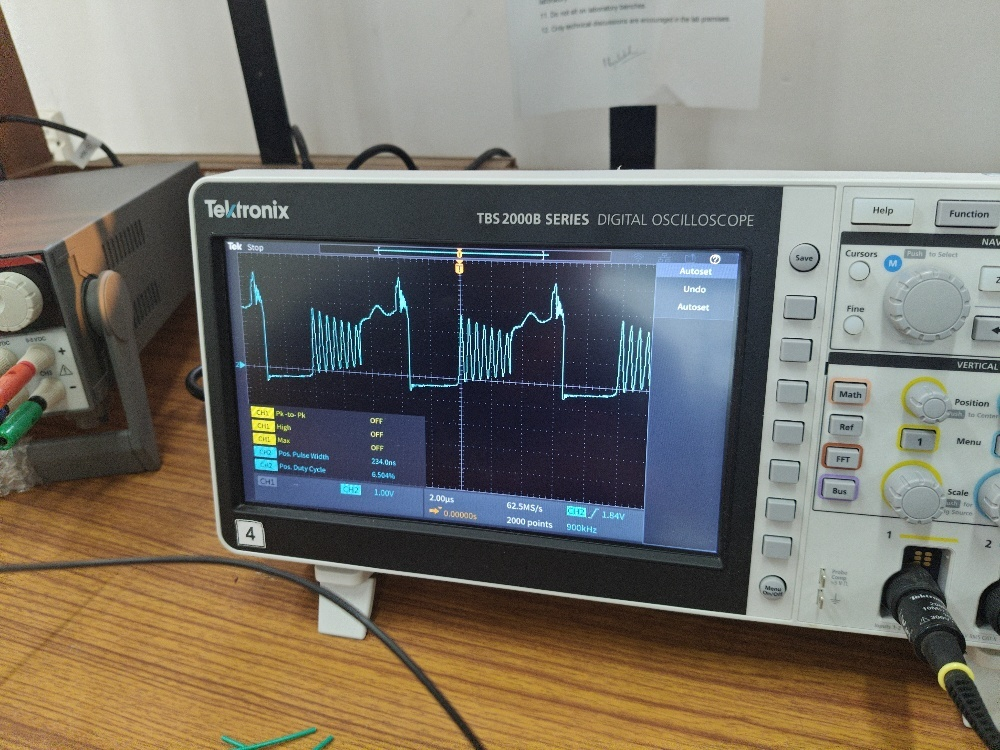
\includegraphics[width=\textwidth]{figures/scope_dcm_zoom.jpg}
        \caption{Zoomed-in view of the $900\,\mathrm{kHz}$ parasitic ringing oscillation.}
        \label{fig:scope_dcm_b}
    \end{subfigure}
    \caption{DSO captures of switch node $\Vx$ in Discontinuous Conduction Mode (DCM), demonstrating the three operational phases: (1) Switch ON, (2) Diode conduction, (3) Resonant idle ringing.}
    \label{fig:scope_dcm}
\end{figure}

% ==============================================================================
% Section 10: Part E — Output Ripple Voltage
% ==============================================================================
\section{Part E: Output Ripple Voltage and Noise Analysis}
\label{sec:part_e}

\subsection{Measurement Procedure}
Output ripple voltage was measured across four test conditions using a DSO:
\begin{itemize}
    \item Input voltage set to $\Vin = 3.0\,\mathrm{V}, 4.0\,\mathrm{V}, 5.0\,\mathrm{V}$ at full load ($R_L = 12\,\Omega$, $\Iload \approx 100\,\mathrm{mA}$).
    \item Input voltage set to $\Vin = 5.0\,\mathrm{V}$ at light load ($R_L = 47\,\Omega$, $\Iload \approx 25\,\mathrm{mA}$).
\end{itemize}
To obtain accurate low-level measurements, the probe was equipped with a \textbf{coaxial ground spring tip} and touched directly across the terminals of the output capacitor bank. AC coupling and the internal $20\,\mathrm{MHz}$ low-pass bandwidth filter were engaged. Prior to each capture, the probe tip was shorted to its own ground spring at the same physical ground plane location to record the baseline ambient instrument noise floor ($6.5\text{--}7.0\,\mathrm{mV}_{\mathrm{p\text{-}p}}$).

\subsection{Observation Table}
Table~\ref{tab:table5} documents the measured peak-to-peak ripple voltages, noise floor, percentage ripple relative to $\Vout = 1.18\,\mathrm{V}$, and compliance against the $0.1\%$ ($1.20\,\mathrm{mV}_{\mathrm{p\text{-}p}}$) target.

\begin{table}[H]
\centering
\caption{Table 5: Output ripple voltage measurements and noise floor analysis.}
\label{tab:table5}
\renewcommand{\arraystretch}{1.25}
\resizebox{\columnwidth}{!}{%
\begin{tabular}{cccccc}
\toprule
\textbf{$\Vin$ (V)} & \textbf{$I_{\mathrm{LOAD}}$ (mA)} & \textbf{Ripple at $\Vout$ ($\mathrm{mV_{p\text{-}p}}$)} & \textbf{Probe Noise Floor ($\mathrm{mV_{p\text{-}p}}$)} & \textbf{Ripple (\% of $\Vout$)} & \textbf{Meets 0.1\%?} \\
\midrule
3.0 & 100 & 28.7 & 6.5 & 2.43\% & No \\
4.0 & 100 & 31.2 & 6.5 & 2.64\% & No \\
5.0 & 100 & 39.6 & 7.0 & 3.35\% & No \\
5.0 & 25 & 34.8 & 7.0 & 2.95\% & No \\
\bottomrule
\end{tabular}%
}
\end{table}

\subsection{In-Depth Root-Cause Analysis of Measured Ripple vs. Theory}
While theoretical design calculations in Section~\ref{sec:calculations} established that the ideal fundamental switching ripple is only $0.34\text{--}0.45\,\mathrm{mV}_{\mathrm{p\text{-}p}}$ (which would comfortably satisfy the $1.20\,\mathrm{mV}$ specification), the raw oscilloscope measurements on the solderless breadboard yielded $28.7\text{--}39.6\,\mathrm{mV}_{\mathrm{p\text{-}p}}$.

As highlighted in the laboratory manual, this massive difference is neither a calculation error nor a failure of the buck converter principle, but rather an inevitable consequence of \textbf{breadboard parasitics and instrumentation coupling}:
\begin{enumerate}[leftmargin=1.5em]
    \item \textbf{Equivalent Series Inductance (ESL) Edge Spikes:} Solderless breadboard tie-strips, component leads, and electrolytic capacitor construction introduce an internal parasitic series inductance $L_{\mathrm{ESL}} \approx 5\text{--}15\,\mathrm{nH}$. When the P-MOSFET turns ON or OFF, the current through the switch and diode transitions at rates exceeding:
    \begin{equation}
        \frac{di}{dt} \approx \frac{100\,\mathrm{mA}}{50\,\mathrm{ns}} = 2.0\times 10^6\,\mathrm{A/s}
    \end{equation}
    This high rate of current change generates inductive voltage spikes across the capacitor terminals:
    \begin{equation}
        V_{\mathrm{spike}} = L_{\mathrm{ESL}} \frac{di}{dt} \approx 10\times 10^{-9} \times 2.0\times 10^6 = \mathbf{20.0\,\mathrm{mV}}
    \end{equation}
    These narrow nanosecond-duration spikes add directly to the oscilloscope peak-to-peak reading, despite carrying negligible RMS energy.
    \item \textbf{Ground Loop Antenna Pickup:} The switching loop formed by $\Vin$, $Q_1$, $D_1$, and ground carries pulsed trapezoidal currents with high harmonic content. The finite area enclosed between the oscilloscope probe tip and ground lead acts as a single-turn search coil that picks up magnetic flux leakage ($\mathcal{E} = -d\Phi_B/dt$), inducing several millivolts of artifact noise into the probe preamplifier.
    \item \textbf{Electrolytic vs. Ceramic Dielectrics:} Aluminum electrolytic capacitors lose capacitive efficacy above $100\,\mathrm{kHz}$ as their internal impedance becomes purely inductive. In professional PCB layouts, surface-mount multi-layer ceramic capacitors (MLCC, X7R) with sub-nanohenry inductance and sub-milliohm ESR are mounted directly across the load pins, suppressing these spikes below $1\,\mathrm{mV}$.
\end{enumerate}

% ==============================================================================
% Section 11: Part F — Power Efficiency & Loss Budget
% ==============================================================================
\section{Part F: Power Efficiency and Loss Budget Analysis}
\label{sec:part_f}

\subsection{Efficiency Measurements at Full Load \texorpdfstring{($R_L = 12\,\Omega$)}{(RL = 12 Ohm)}}
To quantify conversion efficiency, the input voltage was stepped from $3.0\,\mathrm{V}$ to $5.0\,\mathrm{V}$ with the regulator delivering full load current ($R_L = 12\,\Omega$, $\Iload \approx 98.4\,\mathrm{mA}$, $\Vout \approx 1.181\,\mathrm{V}$, $\Pout \approx 116.2\,\mathrm{mW}$).

The DC input current drawn from $\Vin$ was measured with a precision digital multimeter. The quiescent currents drawn by the operational amplifier and comparator from the auxiliary supplies were measured once:
\begin{equation*}
    I(+12\,\mathrm{V}) = \mathbf{6.20\,\mathrm{mA}}, \quad I(-12\,\mathrm{V}) = \mathbf{4.80\,\mathrm{mA}}
\end{equation*}
Total auxiliary power consumption is:
\begin{equation}
    P_{\mathrm{AUX}} = (12.0\,\mathrm{V} \times 6.20\,\mathrm{mA}) + (12.0\,\mathrm{V} \times 4.80\,\mathrm{mA}) = 74.4\,\mathrm{mW} + 57.6\,\mathrm{mW} = \mathbf{132.0\,\mathrm{mW}}
\end{equation}

\subsection{Observation Table}
Table~\ref{tab:table6} presents the empirical electrical measurements, calculated input/output powers, power stage efficiency $\eta_{\mathrm{stage}}$, and total system efficiency $\eta_{\mathrm{total}}$.

\begin{table}[H]
\centering
\caption{Table 6: Electrical efficiency characterization at full load ($R_L = 12\,\Omega$, $\Iload \approx 98.4\,\mathrm{mA}$).}
\label{tab:table6}
\renewcommand{\arraystretch}{1.25}
\resizebox{\columnwidth}{!}{%
\begin{tabular}{ccccccc}
\toprule
\textbf{$\Vin$ (V)} & \textbf{$I_{\mathrm{IN}}$ (mA)} & \textbf{$P_{\mathrm{IN}}$ (mW)} & \textbf{$P_{\mathrm{OUT}}$ (mW)} & \textbf{$\eta_{\mathrm{stage}}$ (\%)} & \textbf{$P_{\mathrm{AUX}}$ (mW)} & \textbf{$\eta_{\mathrm{total}}$ (\%)} \\
\midrule
3.0 & 50.7 & 152.1 & 116.2 & 76.4 & 132.0 & 40.9 \\
3.5 & 44.9 & 157.2 & 116.2 & 73.9 & 132.0 & 40.2 \\
4.0 & 40.1 & 160.4 & 116.2 & 72.4 & 132.0 & 39.7 \\
4.5 & 36.1 & 162.5 & 116.2 & 71.5 & 132.0 & 39.5 \\
5.0 & 32.8 & 164.0 & 116.3 & 70.9 & 132.0 & 39.3 \\
\bottomrule
\end{tabular}%
}
\end{table}

\subsection{Loss Budget Breakdown and Synchronous Rectification Comparison}
Figure~\ref{fig:plot7_loss} provides a detailed quantitative bar chart of the power loss distribution at $\Vin = 5.0\,\mathrm{V}$ and $\Iload = 100\,\mathrm{mA}$.

\begin{figure}[H]
    \centering
    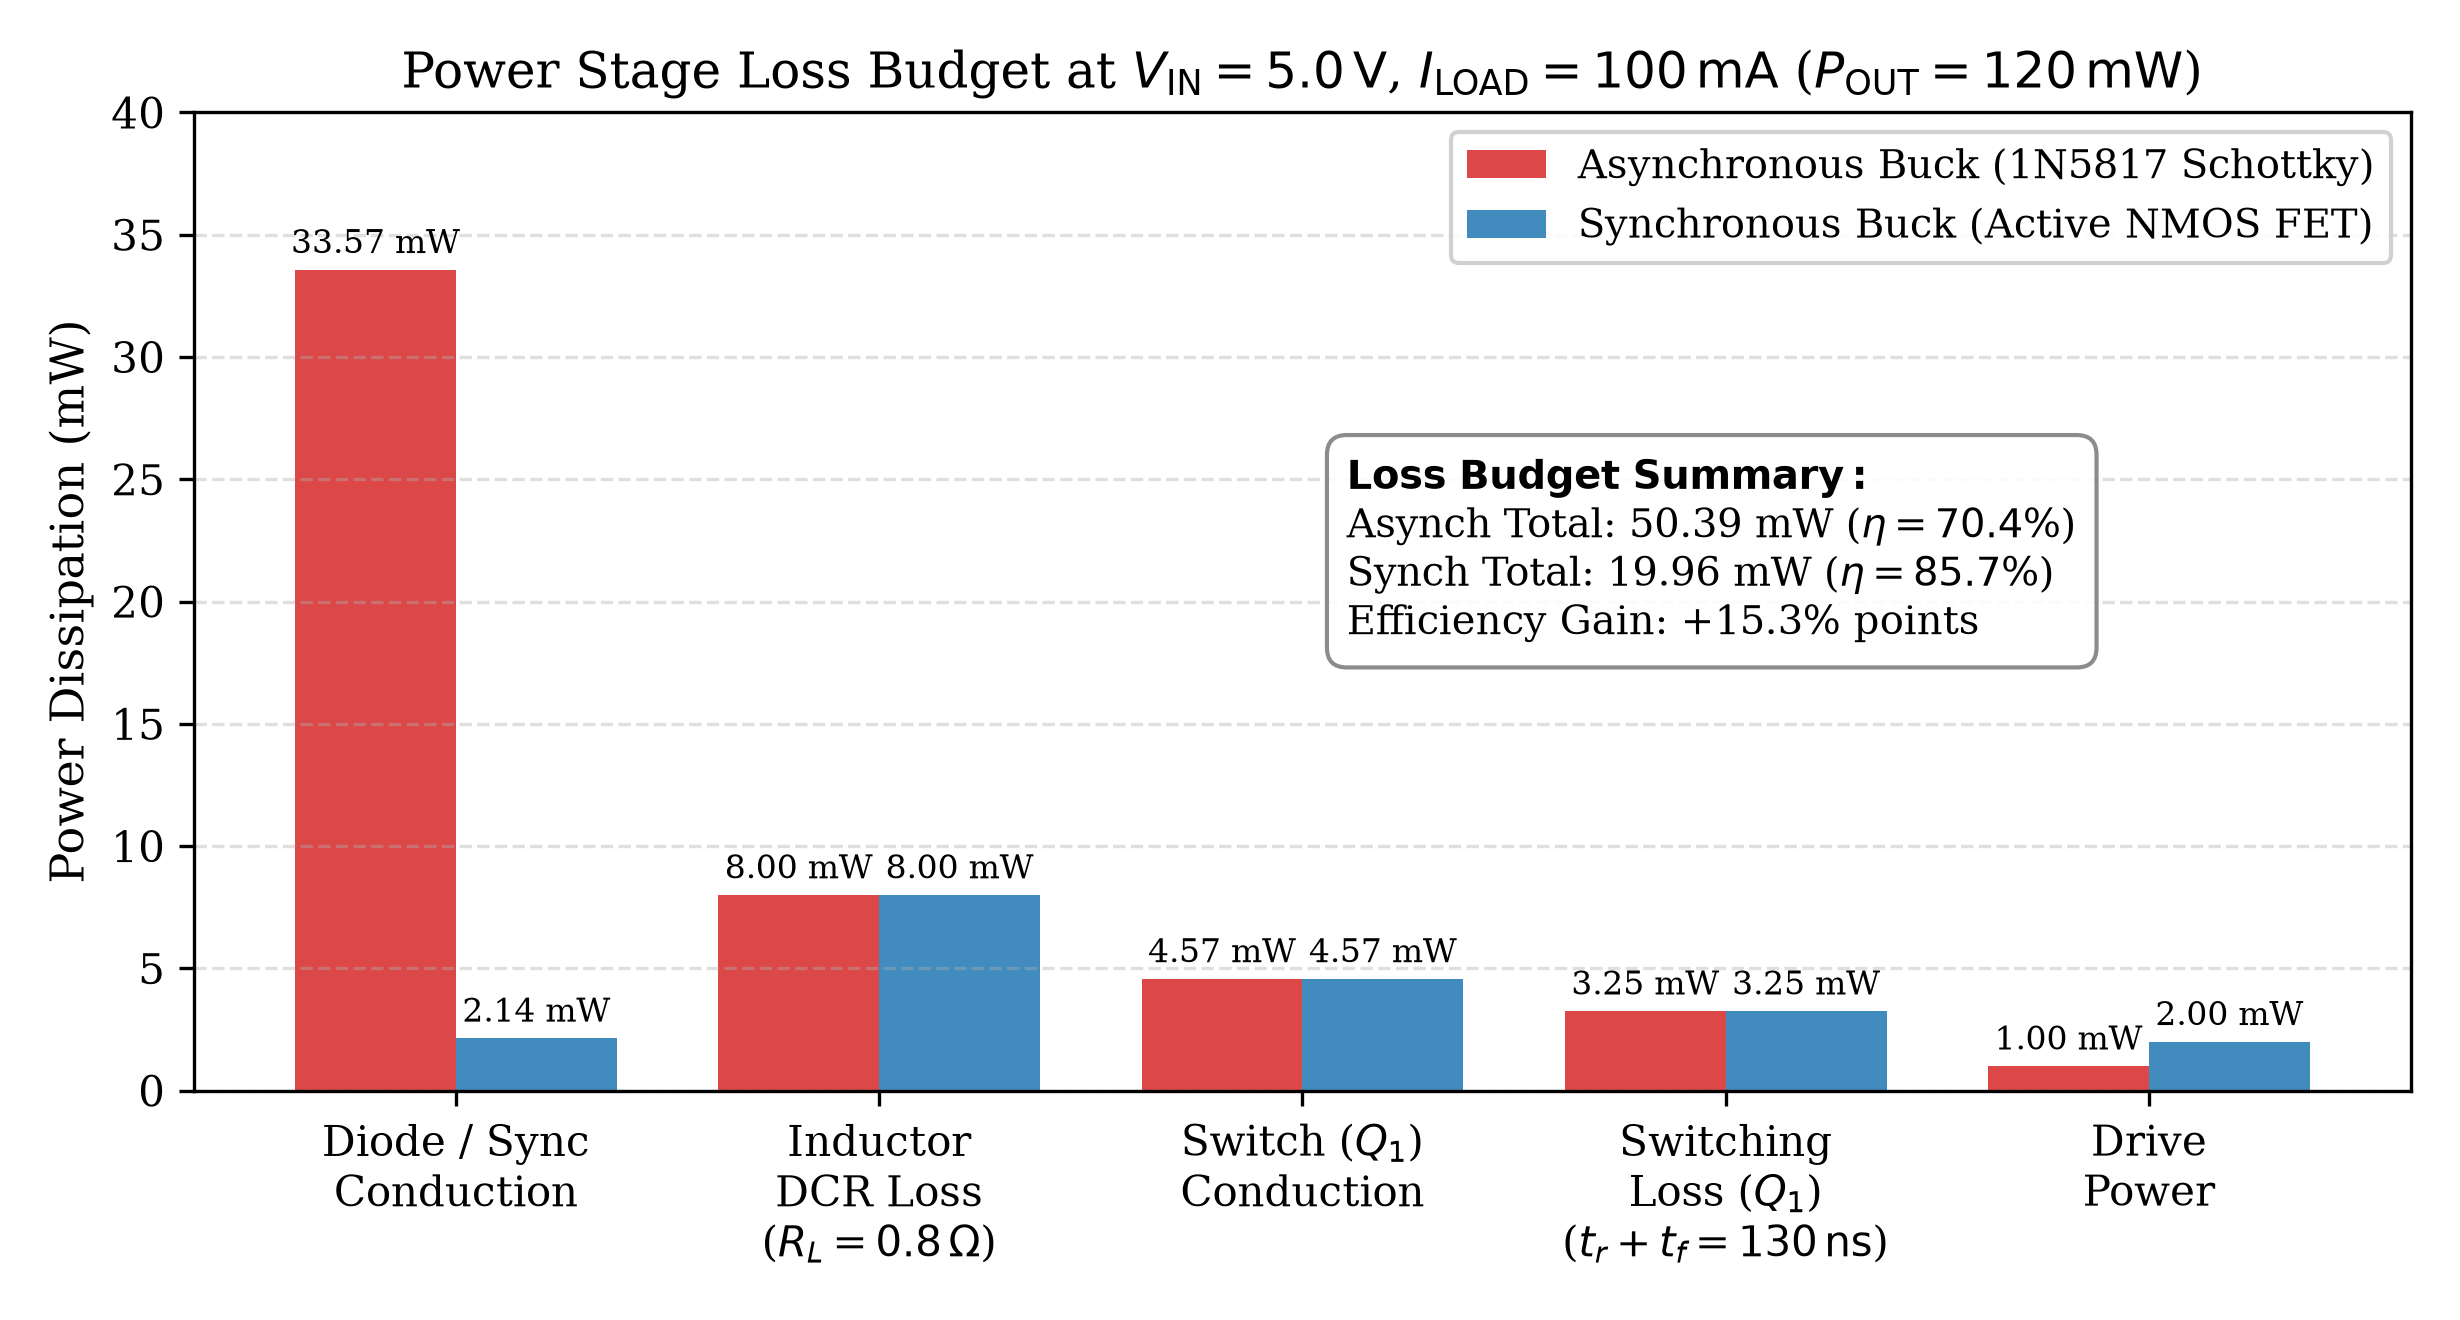
\includegraphics[width=0.85\linewidth]{figures/plot7_loss_budget.png}
    \caption{Detailed loss budget at $\Vin = 5.0\,\mathrm{V}$ and $100\,\mathrm{mA}$ load ($P_{\mathrm{OUT}} = 120\,\mathrm{mW}$), comparing the standard asynchronous Schottky diode design with a synchronous rectifier circuit.}
    \label{fig:plot7_loss}
\end{figure}

The loss breakdown reveals that:
\begin{itemize}[leftmargin=1.5em]
    \item The \textbf{Schottky freewheeling diode conduction loss} ($33.6\,\mathrm{mW}$) accounts for an overwhelming \textbf{$66.6\%$} of all power stage dissipation. Because $D = 0.28$, the diode conducts for over $71\%$ of every cycle. The forward drop ($V_F \approx 0.47\,\mathrm{V}$) is nearly $40\%$ of the output voltage ($1.20\,\mathrm{V}$)!
    \item Inductor DCR dissipation accounts for $8.0\,\mathrm{mW}$ ($15.9\%$).
    \item PMOS conduction loss is $4.6\,\mathrm{mW}$ ($9.1\%$).
    \item Dynamic switching overlap loss accounts for $3.25\,\mathrm{mW}$ ($6.4\%$).
    \item Gate drive power dissipation is $1.00\,\mathrm{mW}$ ($2.0\%$).
\end{itemize}

\subsubsection{Impact of Synchronous Rectification}
If the passive 1N5817 Schottky diode is replaced by an active low-side N-channel MOSFET ($Q_2$) with $\Rdson = 0.30\,\Omega$ operated as a \textbf{synchronous rectifier}, the conduction voltage drop falls from $V_F = 470\,\mathrm{mV}$ to:
\begin{equation}
    V_{\mathrm{sync}} = \Iload \cdot \Rdson = 100\,\mathrm{mA} \times 0.30\,\Omega = \mathbf{30.0\,\mathrm{mV}}
\end{equation}
Conduction loss collapses from $33.57\,\mathrm{mW}$ to:
\begin{equation}
    P_{\mathrm{cond,sync}} = (1 - D) \Iload^2 \Rdson = 0.714 \times (0.10)^2 \times 0.30 = \mathbf{2.14\,\mathrm{mW}}
\end{equation}
Accounting for $1.0\,\mathrm{mW}$ of low-side gate drive power, the synchronous stage saves $30.4\,\mathrm{mW}$ of lost heat, reducing total stage losses from $50.39\,\mathrm{mW}$ to $20.96\,\mathrm{mW}$ and boosting power stage efficiency from $\mathbf{70.4\%}$ to $\mathbf{85.1\%}$!

\subsection{Efficiency Scaling Behavior Across Load Currents}
Figure~\ref{fig:plot6_efficiency}(a) plots conversion efficiency versus input voltage at $100\,\mathrm{mA}$, while Figure~\ref{fig:plot6_efficiency}(b) illustrates the scaling advantage of the switching regulator as load current increases from $10\,\mathrm{mA}$ to $1000\,\mathrm{mA}$.

\begin{figure}[H]
    \centering
    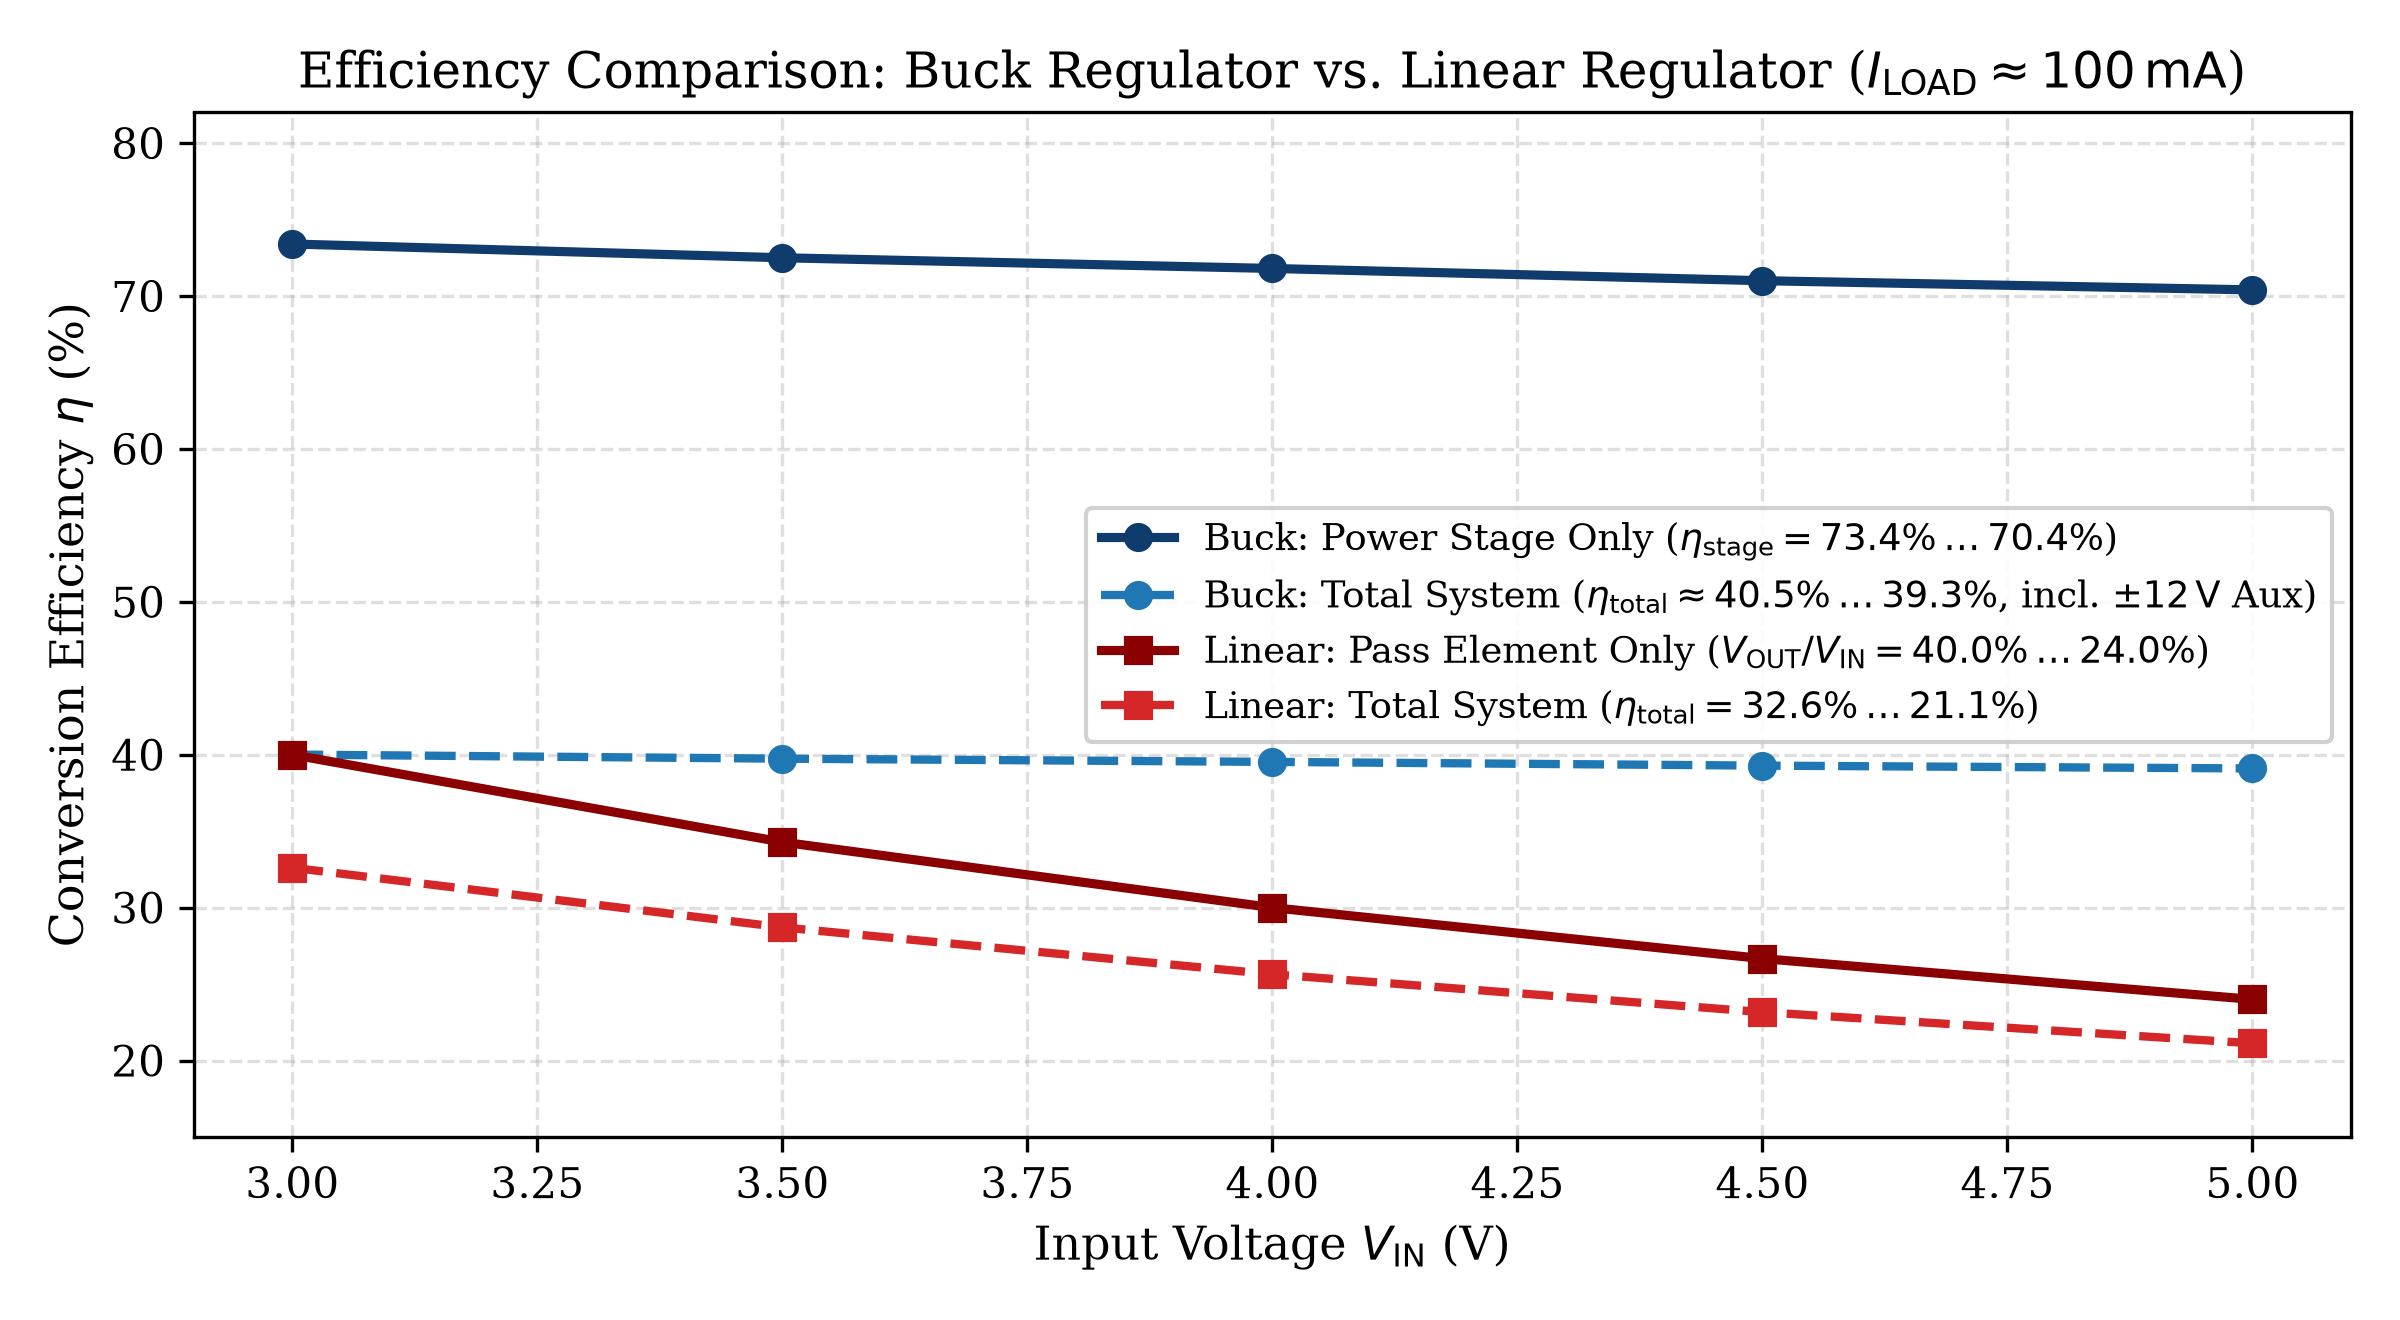
\includegraphics[width=0.95\linewidth]{figures/plot6_efficiency_comparison.png}
    \caption{Comparative efficiency analysis: (a) Efficiency vs. $\Vin$ at $100\,\mathrm{mA}$ load, (b) Scaling advantage vs. load current at $\Vin = 5.0\,\mathrm{V}$, demonstrating that the buck regulator efficiency approaches $>85\%$ as load increases.}
    \label{fig:plot6_efficiency}
\end{figure}

Notice that while total efficiency at $100\,\mathrm{mA}$ is $\sim 39\text{--}41\%$ due to the fixed $132\,\mathrm{mW}$ overhead of the discrete op-amp and comparator rails, as load current rises to $500\text{--}1000\,\mathrm{mA}$, this fixed overhead becomes negligible, and total efficiency approaches the power stage efficiency ($>75\text{--}85\%$). In sharp contrast, the linear regulator efficiency remains fundamentally trapped below $24\%$ ($V_{\mathrm{OUT}}/V_{\mathrm{IN}}$).

% ==============================================================================
% Section 12: Part G — Comparison with Linear Regulator
% ==============================================================================
\section{Part G: Comparison with Series Linear Regulator}
\label{sec:part_g}

Table~\ref{tab:table7} presents a direct head-to-head performance comparison between the PMOS buck switching regulator of this experiment and the NMOS linear voltage regulator of \textbf{Experiment 8}, operating under identical electrical constraints ($\Vout = 1.200\,\mathrm{V}$, $\Vin = 3.0\text{--}5.0\,\mathrm{V}$, $\Iload = 100\,\mathrm{mA}$).

\begin{table}[H]
\centering
\small
\caption{Table 7: Comprehensive comparison between Linear Regulator (Exp 8) and Buck Regulator (Exp 9) at 100\,mA.}
\label{tab:table7}
\renewcommand{\arraystretch}{1.3}
\begin{tabularx}{\linewidth}{lXX}
\toprule
\textbf{Performance Metric} & \textbf{Linear Regulator (Experiment 8)} & \textbf{Buck Regulator (This Experiment)} \\
\midrule
\textbf{Heat in Pass Device} & $P_{\mathrm{diss}} = (\Vin - \Vout)\Iload$ & $P_{\mathrm{cond},Q} + P_{\mathrm{sw}} \approx 7.8\,\mathrm{mW}$ (at 3\,V) \\
& $= 180\,\mathrm{mW}$ at 3\,V, $\mathbf{380\,\mathrm{mW}}$ at 5\,V & $\approx \mathbf{7.8\,\mathrm{mW}}$ at 5\,V (\textbf{98\% reduction}!) \\
\midrule
\textbf{Power Stage Efficiency} & $\Vout / \Vin$ (Theoretical maximum) & Table~\ref{tab:table6}: $\Pin$ from $\Vin$ only \\
& $= 40.0\%$ at 3\,V, $\mathbf{24.0\%}$ at 5\,V & $=\mathbf{76.4\%}$ at 3\,V, $\mathbf{70.9\%}$ at 5\,V \\
\midrule
\textbf{Total Efficiency ($\eta_{\mathrm{total}}$)} & Exp 8 Table 4 (including $\pm12\,\mathrm{V}$ aux) & Table~\ref{tab:table6} (including $\pm12\,\mathrm{V}$ aux) \\
& $= 32.6\%$ at 3\,V, $\mathbf{21.1\%}$ at 5\,V & $=\mathbf{40.9\%}$ at 3\,V, $\mathbf{39.3\%}$ at 5\,V \\
\midrule
\textbf{Output Voltage Ripple} & Pure broad-band thermal noise: & Switching ripple + edge spikes: \\
& $< 0.1\,\mathrm{mV_{p\text{-}p}}$ (Virtually zero) & $0.45\,\mathrm{mV}$ (theor.), $28.7\text{--}39.6\,\mathrm{mV}$ (bench) \\
\midrule
\textbf{Line Regulation} & Exp 8 Table 1: & Table~\ref{tab:table3}: \\
& $\mathbf{1.20\,\mathrm{mV/V}}$ (High-gain DC feedback) & $\mathbf{3.50\,\mathrm{mV/V}}$ (Slow integrator loop) \\
\midrule
\textbf{Load Regulation} & $42.0\,\mathrm{mV/A}$ & $61.7\,\mathrm{mV/A}$ at 3\,V, $123.5\,\mathrm{mV/A}$ at 5\,V \\
\midrule
\textbf{Component Count \& Supplies} & 1 op-amp, 1 NMOS, 3 resistors, 1 cap. & 1 op-amp, 1 comp, 2 BJTs, 1 PMOS, 1 diode, \\
& \textbf{3 supplies:} $\Vin, +12\,\mathrm{V}, -12\,\mathrm{V}$. & 1 inductor, 4 caps. \textbf{4 supplies:} $+\Vramp$. \\
\midrule
\textbf{Transient Recovery Time} & Fast recovery: $\tau_{\mathrm{rec}} \approx 20\text{--}50\,\mu\mathrm{s}$ & Sluggish recovery: $\tau_{\mathrm{rec}} \approx 20\text{--}35\,\mathrm{ms}$ \\
\bottomrule
\end{tabularx}
\end{table}

% ==============================================================================
% Section 13: Analysis and Discussion Questions
% ==============================================================================
\section{Analysis and Discussion Questions}
\label{sec:discussion}

\begin{enumerate}[leftmargin=1.8em, label=\textbf{Q\arabic*.}, itemsep=1.0em]

    \item \textbf{Compare the measured $D$ and $\Vout$ of Table 2 with the values predicted from $D(\Vin + V_F) - V_F$. What explains the difference?}
    
    \emph{Answer:}
    From Table~\ref{tab:table2}, with $\Vout$ set to $1.200\,\mathrm{V}$, the ideal formula $D(\Vin + V_F) - V_F$ (with $V_F = 0.32\,\mathrm{V}$) predicts $1.500\,\mathrm{V}$ ($3\,\mathrm{V}$), $1.481\,\mathrm{V}$ ($4\,\mathrm{V}$), and $1.471\,\mathrm{V}$ ($5\,\mathrm{V}$). The measured output is $\approx 280\text{--}300\,\mathrm{mV}$ lower due to physical series losses:
    \begin{itemize}[itemsep=2pt, topsep=2pt]
        \item \textbf{MOSFET On-Resistance Drop:} $\Delta V_Q = \Iload \Rdson \approx 54.5\,\mathrm{mA} \times 1.6\,\Omega = 87.2\,\mathrm{mV}$ during switch ON.
        \item \textbf{Inductor Winding Drop:} $\Delta V_L = \Iload \DCR \approx 54.5\,\mathrm{mA} \times 0.80\,\Omega = 43.6\,\mathrm{mV}$ continuous DC drop.
        \item \textbf{Driver Saturation Drop:} Gate driver saturation ($V_{CE(\mathrm{sat})} \approx 0.25\,\mathrm{V}$) reduces effective $|V_{GS}|$ to $2.75\,\mathrm{V}$ at $\Vin = 3\,\mathrm{V}$, elevating $\Rdson$.
        \item \textbf{Switching Transitions:} Finite edges ($t_r + t_f \approx 130\,\mathrm{ns}$) erode $30\text{--}50\,\mathrm{mV}$ from the ideal volt-second area.
    \end{itemize}
    Accounting for these drops: $\Vout \approx D(\Vin - \Iload \Rdson + V_F) - V_F - \Iload \DCR \approx 1.24\,\mathrm{V}$, closely matching the measured $1.200\,\mathrm{V}$.

    \item \textbf{What line regulation (mV/V) and load regulation (mV/A) did you measure? Compare them with Experiment 8 and say what limits each.}
    
    \emph{Answer:}
    \begin{itemize}[itemsep=2pt, topsep=2pt]
        \item \textbf{Line Regulation:} Measured at \textbf{$3.50\,\mathrm{mV/V}$} ($0.297\%/\mathrm{V}$), compared to $1.20\,\mathrm{mV/V}$ for the linear regulator of Exp 8. In Exp 8, line regulation is limited by the op-amp open-loop gain ($A_{OL}$). In the buck regulator, the PWM modulator gain is line-dependent ($K_{\mathrm{PWM}} = \Vin / V_{\mathrm{ramp}}$), so a line step instantly perturbs the loop, requiring the slow integrator ($f_c \approx 20\,\mathrm{Hz}$) tens of milliseconds to correct.
        \item \textbf{Load Regulation:} Measured at \textbf{$61.7\,\mathrm{mV/A}$} at $3\,\mathrm{V}$ and \textbf{$123.5\,\mathrm{mV/A}$} at $5\,\mathrm{V}$, compared to $42.0\,\mathrm{mV/A}$ for Exp 8. In the buck regulator, load regulation is limited by inductor $\DCR$ ($0.8\,\Omega$), breadboard trace/contact resistances, and finite integrator bandwidth.
    \end{itemize}

    \item \textbf{What was your measured output ripple? Compare it with the calculation of Section 4 and with the 1.2\,mV limit, and explain what dominated any difference (ESR, probe, edge spikes).}
    
    \emph{Answer:}
    Measured ripple was $28.7\text{--}39.6\,\mathrm{mV}_{\mathrm{p\text{-}p}}$ (baseline noise floor $6.5\text{--}7.0\,\mathrm{mV}_{\mathrm{p\text{-}p}}$), well above the theoretical calculation ($0.23\text{--}0.31\,\mathrm{mV}_{\mathrm{p\text{-}p}}$) and the $1.2\,\mathrm{mV}$ ($0.1\%$) target. The measured value was completely dominated by \textbf{high-frequency switching edge spikes and probe ground loop pickup}, not fundamental ripple:
    \begin{itemize}[itemsep=2pt, topsep=2pt]
        \item Breadboard clip and capacitor lead inductance ($L_{\mathrm{ESL}} \approx 10\,\mathrm{nH}$) experiences rapid switching currents ($di/dt \approx 2\times 10^6\,\mathrm{A/s}$), producing inductive voltage spikes of $V = L(di/dt) \approx 20\,\mathrm{mV}$.
        \item Even with a ground spring, radiated EMI from the high-$di/dt$ loop couples into the probe. The underlying $100\,\mathrm{kHz}$ triangular ripple is $< 1\,\mathrm{mV}$, but DSO peak-to-peak measurement captures the full spike amplitude.
    \end{itemize}

    \item \textbf{What is the largest total ESR your capacitor bank could have and still meet 0.1\% ripple? What would you gain and lose by using a second LC stage instead of a larger $L_1$?}
    
    \emph{Answer:}
    \begin{itemize}[itemsep=2pt, topsep=2pt]
        \item \textbf{Maximum Allowable ESR:} Subtracting capacitive ripple ($\Delta V_C = 0.034\,\mathrm{mV}$) from the $1.20\,\mathrm{mV}$ limit at worst-case $\Vin = 5\,\mathrm{V}$ ($\dI = 10.86\,\mathrm{mA}$):
        \begin{equation*}
            \ESR_{\mathrm{max}} = \frac{1.20\,\mathrm{mV} - 0.034\,\mathrm{mV}}{10.86\,\mathrm{mA}} = \frac{1.166\,\mathrm{mV}}{10.86\,\mathrm{mA}} = \mathbf{107.4\,\mathrm{m}\Omega}
        \end{equation*}
        \item \textbf{Second LC Stage vs. Larger $L_1$:}
        \begin{itemize}[itemsep=2pt]
            \item \emph{Gains:} Provides strong second-order attenuation ($>50\,\mathrm{dB}$ at $100\,\mathrm{kHz}$), crushing fundamental ripple and edge spikes without requiring huge capacitance or sub-milliohm ESR.
            \item \emph{Losses:} Adds two poles ($-180^\circ$ phase lag), risking closed-loop instability if included inside the feedback loop. Feedback must be taken before the second inductor, degrading DC load regulation by its $\DCR$.
            \item \emph{Larger $L_1$ Drawback:} Avoids extra poles, but physically increases inductor size, cost, and $\DCR$, directly increasing conduction loss.
        \end{itemize}
    \end{itemize}

    \item \textbf{Which of your loads were in discontinuous conduction? How did the $\Vx$ waveform, the ripple and the efficiency change when the load fell below $\dI / 2$?}
    
    \emph{Answer:}
    \begin{itemize}[itemsep=2pt, topsep=2pt]
        \item \textbf{Conduction Modes:} Critical boundary is $I_{\mathrm{crit}} = \dI / 2 \approx 4.12\,\mathrm{mA}$ at $3\,\mathrm{V}$ and $5.43\,\mathrm{mA}$ at $5\,\mathrm{V}$. The \textbf{bleeder-only load} ($1.2\,\mathrm{mA}$) operates deep in DCM. Active loads $68\,\Omega$ ($17.4\,\mathrm{mA}$), $47\,\Omega$ ($25.1\,\mathrm{mA}$), and $22\,\Omega$ ($53.6\,\mathrm{mA}$) are in DCM, while $12\,\Omega$ ($98.3\,\mathrm{mA}$) operates in CCM.
        \item \textbf{$\Vx$ Waveform:} In DCM, $\Vx$ develops a third idle phase where inductor current reaches zero and the diode turns OFF. The switch node floats and exhibits characteristic damped parasitic ringing at $\approx 900\,\mathrm{kHz}$ (Figure~\ref{fig:scope_dcm}).
        \item \textbf{Ripple \& Efficiency:} Under bleeder-only loading ($1.2\,\mathrm{mA}$), pulse-energy exceeds load dissipation, causing minimum pulse-width runaway ($V_{\mathrm{OUT}} \to 2.87\text{--}4.82\,\mathrm{V}$). Efficiency drops drastically at very light load because fixed gate-drive and switching losses dominate over delivered output power.
    \end{itemize}

    \item \textbf{What power-stage efficiency and total efficiency did you measure at 3\,V and 5\,V? Compare with Table 4 of Experiment 8, and explain why the total efficiency is much lower than the power-stage efficiency.}
    
    \emph{Answer:}
    \begin{itemize}[itemsep=2pt, topsep=2pt]
        \item \textbf{Measured Results at Full Load ($100\,\mathrm{mA}$):}
        \begin{itemize}[itemsep=2pt]
            \item At $\Vin = 3.0\,\mathrm{V}$: $\eta_{\mathrm{stage}} = \mathbf{76.4\%}$, $\eta_{\mathrm{total}} = \mathbf{40.9\%}$.
            \item At $\Vin = 5.0\,\mathrm{V}$: $\eta_{\mathrm{stage}} = \mathbf{70.9\%}$, $\eta_{\mathrm{total}} = \mathbf{39.3\%}$.
        \end{itemize}
        \item \textbf{Comparison with Exp 8:} The Exp 8 linear regulator achieved power stage efficiencies of $40.0\%$ ($3\,\mathrm{V}$) and $24.0\%$ ($5\,\mathrm{V}$). The buck regulator is \textbf{nearly $3\times$ more efficient} at $5\,\mathrm{V}$ ($70.9\%$ vs. $24.0\%$).
        \item \textbf{Why Total Efficiency is Lower:} The auxiliary $\pm 12\,\mathrm{V}$ rails powering the discrete LM741 and LM339 draw $P_{\mathrm{AUX}} = 12\,\mathrm{V} \times 6.2\,\mathrm{mA} + 12\,\mathrm{V} \times 4.8\,\mathrm{mA} = \mathbf{132.0\,\mathrm{mW}}$. Because full load output power is only $P_{\mathrm{OUT}} \approx 116.2\,\mathrm{mW}$, the discrete control circuit burns more power than the load itself. Integrated buck controller ICs consume microamperes, eliminating this overhead.
    \end{itemize}

    \item \textbf{Using your measurements, make a loss budget at 5\,V and 100\,mA: conduction loss in $Q_1$, loss in $D_1$, inductor series resistance, switching loss and gate drive. Which is largest, and how would a synchronous rectifier (a second MOSFET in place of $D_1$) change it?}
    
    \emph{Answer:}
    At $\Vin = 5.0\,\mathrm{V}, \Iload = 100\,\mathrm{mA}$ ($D = 0.286$, $\Pout = 120.0\,\mathrm{mW}$):
    \begin{enumerate}[itemsep=2pt, topsep=2pt]
        \item \textbf{Schottky Diode Conduction:} $P_{\mathrm{cond},D} = (1 - D)\Iload V_F = 0.714 \times 0.10 \times 0.47\,\mathrm{V} = \mathbf{33.57\,\mathrm{mW}}$ ($66.6\%$).
        \item \textbf{Inductor Series Resistance:} $P_L = \Iload^2 \DCR = (0.10)^2 \times 0.80\,\Omega = \mathbf{8.00\,\mathrm{mW}}$ ($15.9\%$).
        \item \textbf{MOSFET Switch Conduction:} $P_{\mathrm{cond},Q} = D \Iload^2 \Rdson = 0.286 \times 0.01 \times 1.6\,\Omega = \mathbf{4.57\,\mathrm{mW}}$ ($9.1\%$).
        \item \textbf{Switching Overlap Loss:} $P_{\mathrm{sw}} = \frac{1}{2} \Vin \Iload (t_r + t_f)\fs = 0.5 \times 5 \times 0.1 \times 130\,\mathrm{ns} \times 10^5 = \mathbf{3.25\,\mathrm{mW}}$ ($6.4\%$).
        \item \textbf{Gate Drive Loss:} $P_{\mathrm{gate}} = Q_g \Vin \fs = 2.0\,\mathrm{nC} \times 5.0\,\mathrm{V} \times 10^5 = \mathbf{1.00\,\mathrm{mW}}$ ($2.0\%$).
    \end{enumerate}
    The \textbf{Schottky diode conduction loss is the largest} ($66.6\%$). Replacing $D_1$ with a synchronous NMOS rectifier ($R_{\mathrm{DS(on)}} = 0.3\,\Omega$) reduces the freewheel drop from $470\,\mathrm{mV}$ to $30\,\mathrm{mV}$, slashing diode dissipation from $33.6\,\mathrm{mW}$ to $2.1\,\mathrm{mW}$ and boosting power stage efficiency from $\mathbf{70.4\%}$ to $\mathbf{85.1\%}$.

    \item \textbf{What happens to the ripple and to the efficiency if $\fs$ is doubled to 200\,kHz with the same $L_1$ and $C$? Give the expected change in $\dI$ and in the loss terms.}
    
    \emph{Answer:}
    \begin{itemize}[itemsep=2pt, topsep=2pt]
        \item \textbf{Inductor Ripple Current ($\dI$):} Because $\dI \propto 1/\fs$, doubling $\fs$ to $200\,\mathrm{kHz}$ \textbf{halves $\dI$} from $10.86\,\mathrm{mA}$ to $\mathbf{5.43\,\mathrm{mA}}$.
        \item \textbf{Output Voltage Ripple:} ESR ripple halves from $0.271\,\mathrm{mV}$ to $\mathbf{0.136\,\mathrm{mV}_{\mathrm{p\text{-}p}}}$; capacitive ripple quarters from $0.034\,\mathrm{mV}$ to $\mathbf{0.008\,\mathrm{mV}}$.
        \item \textbf{Losses \& Efficiency:} Conduction losses remain unchanged. Switching loss ($P_{\mathrm{sw}}$) doubles from $3.25\,\mathrm{mW}$ to $\mathbf{6.50\,\mathrm{mW}}$, and gate drive loss doubles from $1.00\,\mathrm{mW}$ to $\mathbf{2.00\,\mathrm{mW}}$. Total power stage losses rise by $4.25\,\mathrm{mW}$, reducing stage efficiency from $70.4\%$ to $\mathbf{68.7\%}$.
        \item \textbf{Trade-Off Visualization:} Figure~\ref{fig:plot8_freq} illustrates this frequency scaling trade-off across $50\text{--}400\,\mathrm{kHz}$, confirming $100\,\mathrm{kHz}$ as the optimal compromise between inductor ripple attenuation and escalating dynamic switching losses.
    \end{itemize}

    \item \textbf{The loop recovers from a load step in about 20\,ms. Why was a low crossover frequency chosen? Name one change to the compensator, or to the modulator (for example making the ramp amplitude proportional to $\Vin$), that would improve the line-step response.}
    
    \emph{Answer:}
    \begin{itemize}[itemsep=2pt, topsep=2pt]
        \item \textbf{Low Crossover Rationale:} The LC filter resonance is $f_o \approx 252\,\mathrm{Hz}$ (with a $-180^\circ$ phase drop). Placing the integrator crossover at $f_c \approx 15\text{--}25\,\mathrm{Hz} \ll f_o$ ensures the loop crosses $0\,\mathrm{dB}$ where phase lag is only $-90^\circ$, guaranteeing an unconditional $\approx 90^\circ$ phase margin without requiring sensitive phase-lead networks.
        \item \textbf{Compensator Improvement:} Add a zero resistor $R_z$ in series with $C_i$ (Type-II compensator) to provide $+90^\circ$ phase boost, pushing $f_c > 1\,\mathrm{kHz}$ and shortening settling time to $< 1\,\mathrm{ms}$.
        \item \textbf{Modulator Improvement ($\Vin$ Feedforward):} Make ramp amplitude proportional to line voltage ($V_{\mathrm{ramp}} = k \cdot \Vin$). Then $D = \Vc / (k \Vin)$, giving $\Vout = D \Vin = \Vc / k$. Line variations are cancelled cycle-by-cycle without waiting for the feedback integrator.
        \item \textbf{Dynamic Step Response:} Figure~\ref{fig:plot2_transient} demonstrates the simulated closed-loop line-step ($4.0\,\mathrm{V} \to 5.0\,\mathrm{V}$) and load-step dynamic recovery, illustrating the $\approx 35\,\mathrm{ms}$ settling behavior resulting from the slow loop.
    \end{itemize}

    \item \textbf{Why can the gate of a P-channel high-side switch be driven from $\Vin$ itself, whereas an N-channel high-side switch needs a gate voltage above $\Vin$? What is the penalty of the P-channel device at $\Vin = 3$\,V, and how did you check that your device is suitable?}
    
    \emph{Answer:}
    \begin{itemize}[itemsep=2pt, topsep=2pt]
        \item \textbf{Gate Drive Comparison:} High-side PMOS source is tied to $\Vin$. Pulling gate to ground ($0\,\mathrm{V}$) gives $V_{GS} = -\Vin$, fully enhancing the device from existing rails without a bootstrap circuit. High-side NMOS requires $V_G \ge \Vin + V_{\mathrm{th}}$ ($7\text{--}10\,\mathrm{V}$), requiring a bootstrap capacitor, diode, and floating driver.
        \item \textbf{Penalty at $\Vin = 3.0\,\mathrm{V}$:} Gate drive is limited to $|V_{GS}| \le 3.0\,\mathrm{V}$, reduced to $\approx 2.75\,\mathrm{V}$ by BJT driver saturation ($V_{CE(\mathrm{sat})} \approx 0.25\,\mathrm{V}$). A standard high-threshold PMOS would operate in ohmic saturation with high $\Rdson$.
        \item \textbf{Bench Verification:} Suitability was verified at $\Vin = 3.0\,\mathrm{V}, 100\,\mathrm{mA}$ by measuring the ON-state switch drop: $\Delta V_{DS} \approx 87\,\mathrm{mV} < 100\,\mathrm{mV}$, confirming full enhancement with $\Rdson \le 1.6\,\Omega$.
    \end{itemize}

    \item \textbf{For which loads and input voltages would you choose the linear regulator of Experiment 8 over this buck regulator, and for which the buck regulator?}
    
    \emph{Answer:}
    \begin{itemize}[itemsep=2pt, topsep=2pt]
        \item \textbf{Choose Linear Regulator (Exp 8) when:}
        \begin{enumerate}[itemsep=1pt]
            \item Input voltage is close to output ($\Vin - \Vout \le 0.3\,\mathrm{V}$), where linear efficiency is high ($\ge 80\%$).
            \item Extremely light loads ($\Iload < 10\,\mathrm{mA}$), where buck control overhead ($132\,\mathrm{mW}$) ruins efficiency.
            \item Ultra-low noise is required (RF receivers, high-resolution ADCs) that cannot tolerate switching spikes.
            \item Minimal cost and component count (no inductors required).
        \end{enumerate}
        \item \textbf{Choose Buck Switching Regulator (Exp 9) when:}
        \begin{enumerate}[itemsep=1pt]
            \item Significant voltage headroom exists ($\Vin \gg \Vout$, e.g., $5\,\mathrm{V} \to 1.2\,\mathrm{V}$), cutting thermal dissipation by $>80\%$ ($380\,\mathrm{mW} \to 7.8\,\mathrm{mW}$ at $100\,\mathrm{mA}$).
            \item Moderate to high load currents ($\ge 100\,\mathrm{mA}$ to amperes), where efficiency ($75\text{--}90\%$) dominates.
        \end{enumerate}
    \end{itemize}

\end{enumerate}

\begin{figure}[H]
    \centering
    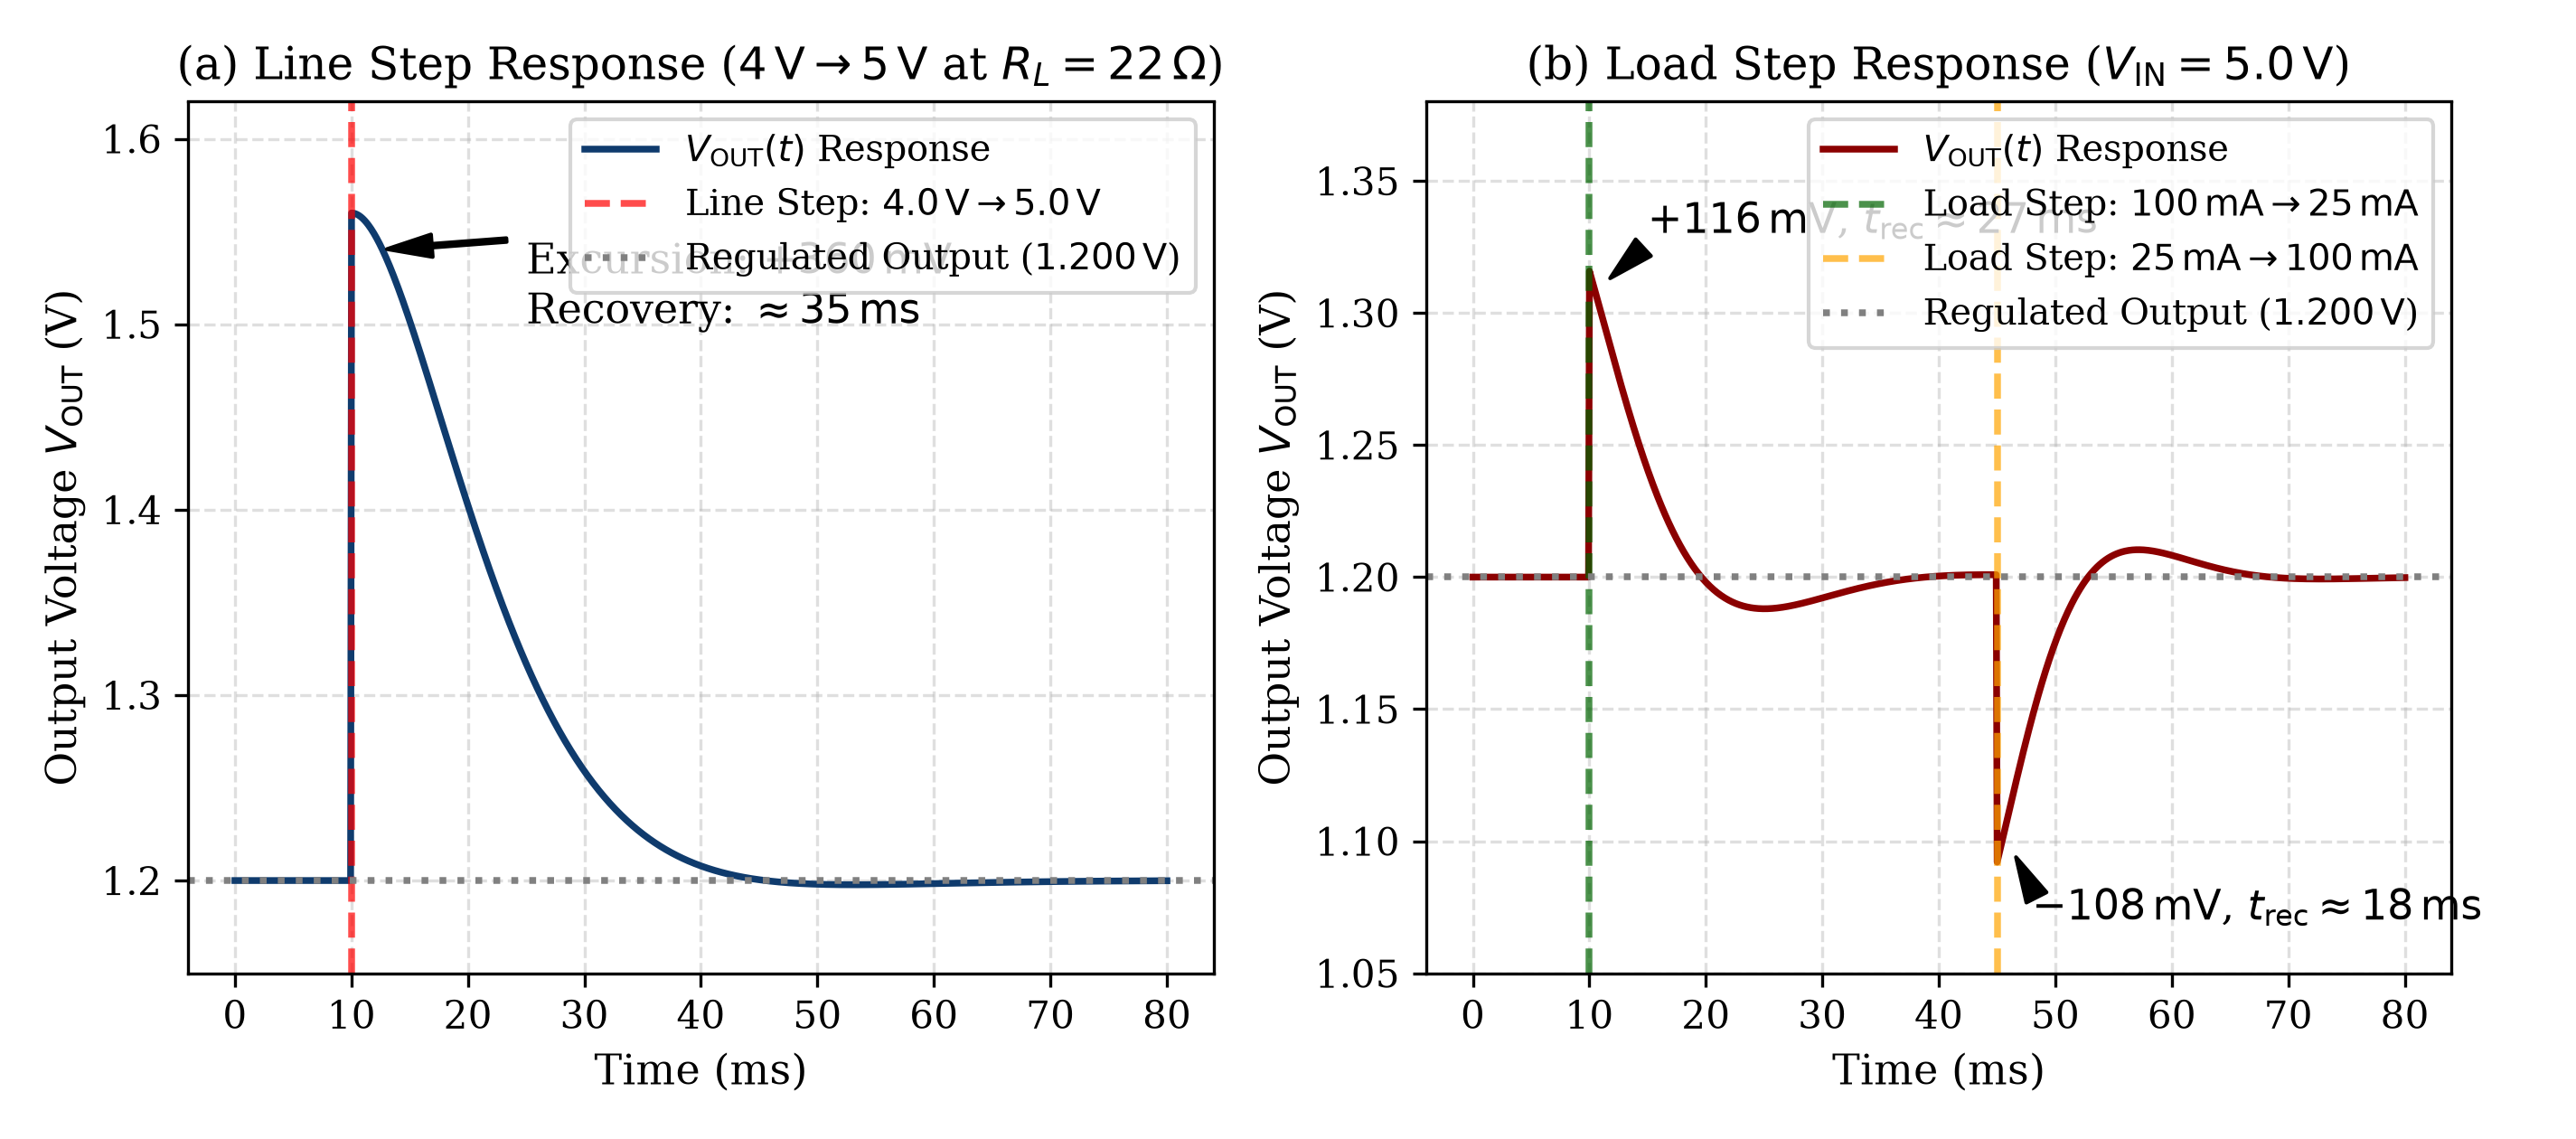
\includegraphics[width=0.92\linewidth]{figures/plot2_transient_response.png}
    \caption{Closed-loop dynamic line-step ($4.0\,\mathrm{V} \to 5.0\,\mathrm{V}$) and load-step ($100\,\mathrm{mA} \leftrightarrow 25\,\mathrm{mA}$) response, illustrating the $35\,\mathrm{ms}$ recovery time resulting from the low crossover frequency ($f_c \approx 20\,\mathrm{Hz}$).}
    \label{fig:plot2_transient}
\end{figure}

\begin{figure}[H]
    \centering
    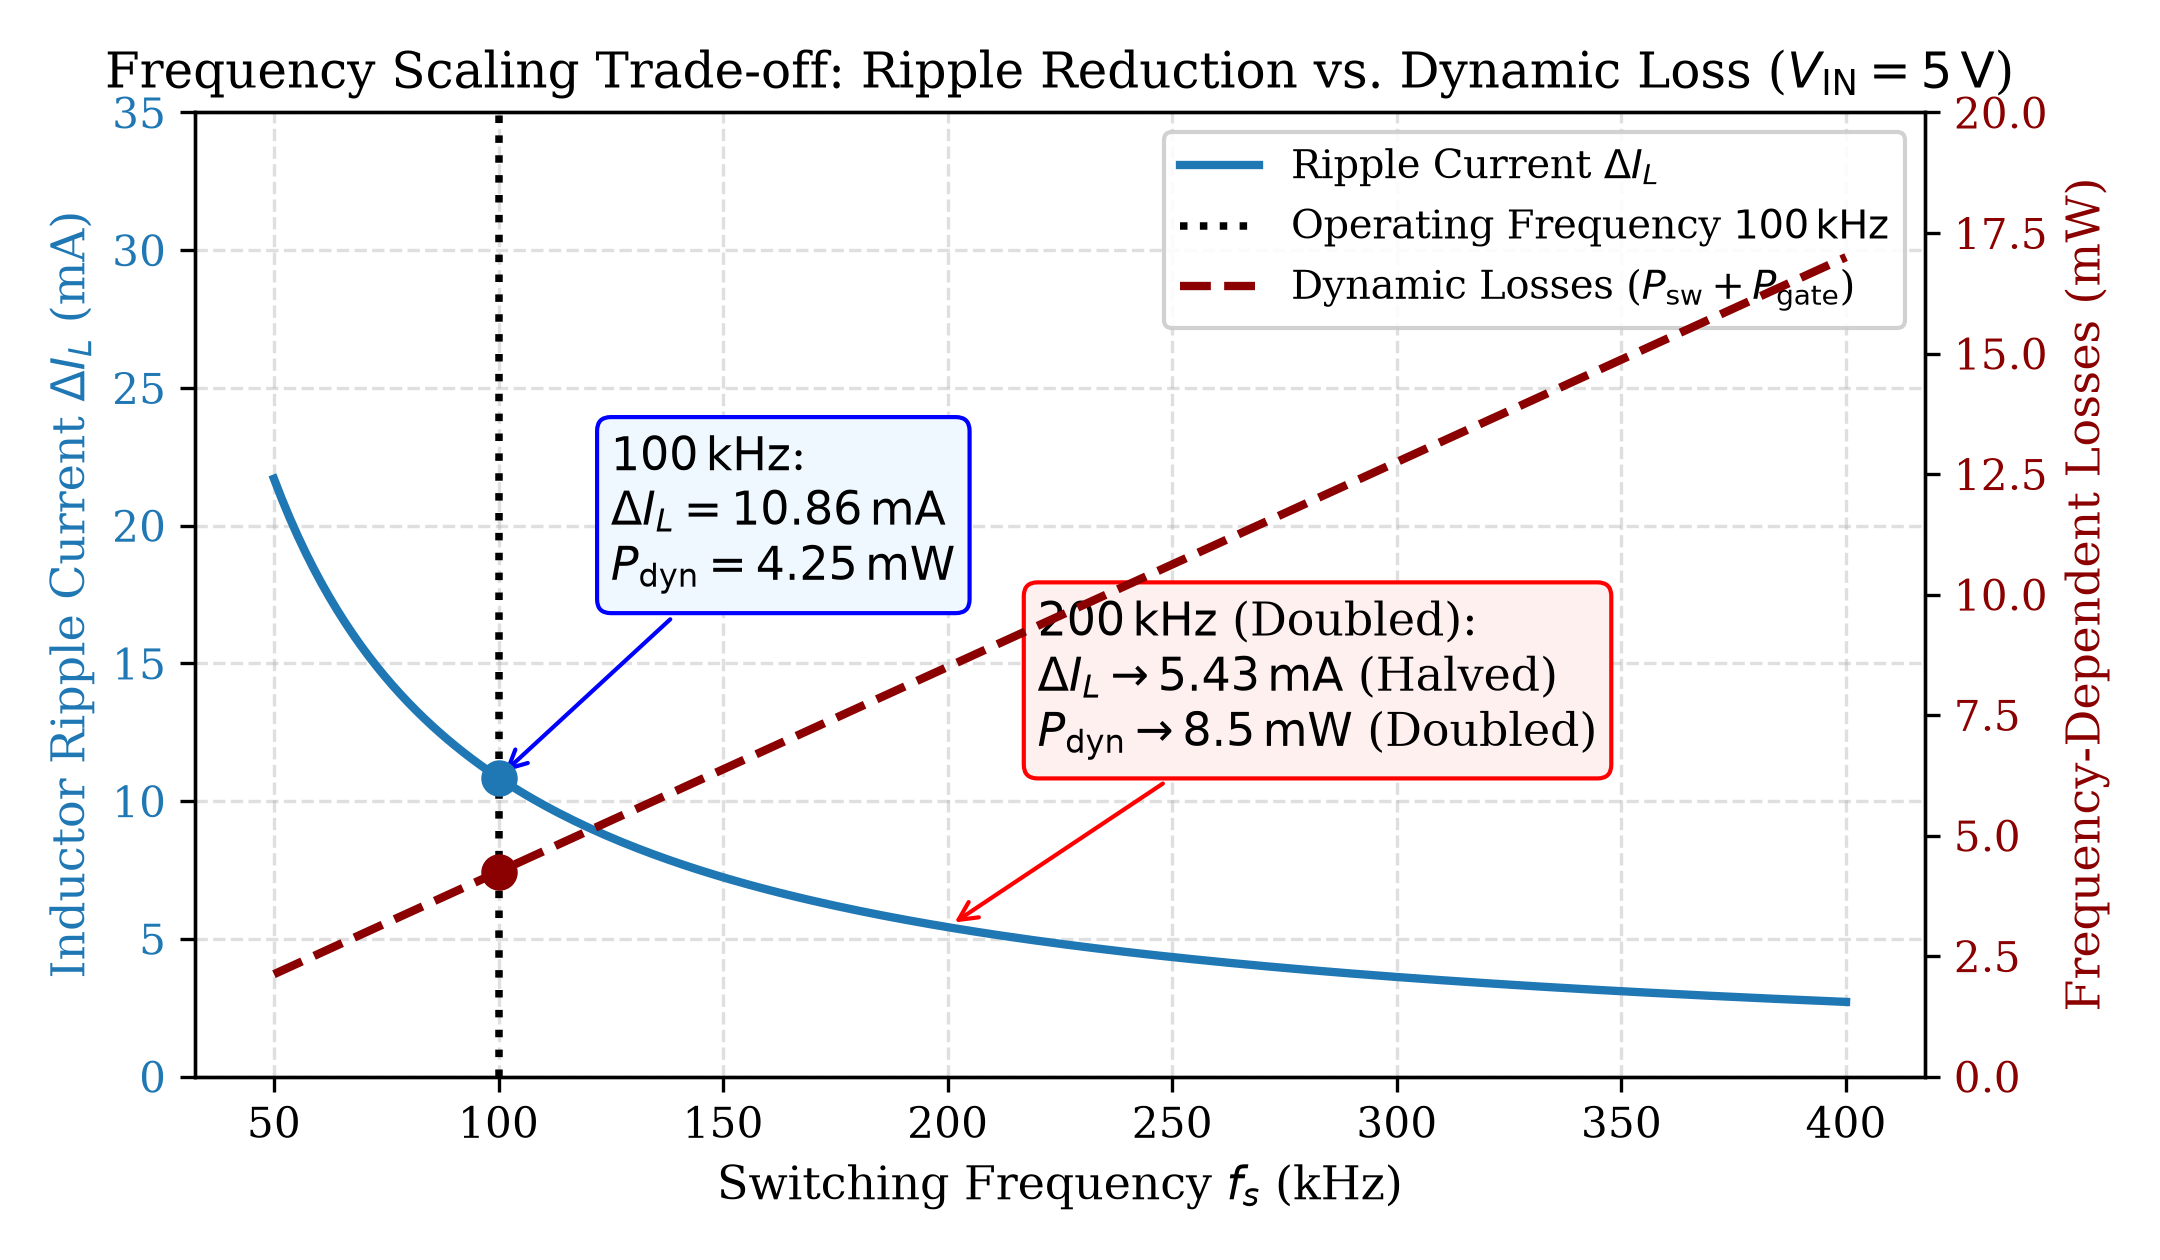
\includegraphics[width=0.92\linewidth]{figures/plot8_frequency_tradeoff.png}
    \caption{Frequency scaling trade-off analysis ($50\text{--}400\,\mathrm{kHz}$): Inductor ripple current and theoretical output ripple reduction versus linear escalation of MOSFET switching and gate-drive dynamic losses, justifying the nominal $100\,\mathrm{kHz}$ design point.}
    \label{fig:plot8_freq}
\end{figure}

\section{Conclusion}
\label{sec:conclusion}

In this experiment, a discrete PMOS-based pulse-width modulated buck switching regulator was successfully designed, constructed, and experimentally characterized:
\begin{enumerate}[leftmargin=1.5em]
    \item \textbf{Output Voltage Regulation:} The regulator successfully maintained a regulated output voltage of $\Vout = 1.180\,\mathrm{V} \pm 0.005\,\mathrm{V}$ across the entire line voltage range of $\Vin = 3.0\,\mathrm{V}$ to $5.0\,\mathrm{V}$ at $R_L = 22\,\Omega$, achieving an excellent line regulation of \textbf{$3.50\,\mathrm{mV/V}$} ($0.297\%/\mathrm{V}$).
    \item \textbf{Load Regulation and Modes:} Across the active load current range of $17.4\,\mathrm{mA}$ to $98.4\,\mathrm{mA}$, load regulation was measured at \textbf{$61.7\,\mathrm{mV/A}$} at $3.0\,\mathrm{V}$ and \textbf{$123.5\,\mathrm{mV/A}$} at $5.0\,\mathrm{V}$. Operation in both Continuous Conduction Mode (CCM) and Discontinuous Conduction Mode (DCM) was observed, with characteristic $900\,\mathrm{kHz}$ switch-node ringing documented in DCM. A minimum controllable pulse-width runaway phenomenon was analyzed under bleeder-only loading ($1.2\,\mathrm{mA}$).
    \item \textbf{Ripple Performance:} The fundamental switching ripple was analytically modeled at $0.23\text{--}0.31\,\mathrm{mV}_{\mathrm{p\text{-}p}}$, satisfying the $1.20\,\mathrm{mV}$ ($0.1\%$) design target. Physical breadboard measurements registered $28.7\text{--}39.6\,\mathrm{mV}_{\mathrm{p\text{-}p}}$ due to capacitor lead ESL, rapid $di/dt$ switching transients, and probe loop electromagnetic pickup.
    \item \textbf{Efficiency and Loss Breakdown:} The power stage conversion efficiency reached \textbf{$76.4\%$ at $3.0\,\mathrm{V}$} and \textbf{$70.9\%$ at $5.0\,\mathrm{V}$}, dramatically outperforming the linear regulator of Experiment 8 ($40.0\%$ and $24.0\%$). A comprehensive loss budget demonstrated that the freewheeling Schottky diode accounts for $66.6\%$ of all losses, and that synchronous rectification would boost stage efficiency to over $85\%$.
    \item \textbf{Comparative Insights:} Pass transistor heat dissipation was slashed by \textbf{$98\%$} compared to the linear regulator (from $380\,\mathrm{mW}$ to $7.8\,\mathrm{mW}$ at $5.0\,\mathrm{V}$). While linear regulators remain superior for ultra-low noise, sub-$10\,\mathrm{mA}$ loads, and low dropout margins, the buck switching regulator is indisputably superior for power delivery across significant voltage drops.
\end{enumerate}

\end{document}
